\documentclass[fleqn,letterpaper]{report}
\usepackage{remhref}
\usepackage{nowidow}

\begin{document}

\title{Course Notes for Calculus IV}
\author{Remkes Kooistra\\
	The King's University}
\date{\today}
\maketitle

\setcounter{tocdepth}{1}
\tableofcontents

\chapter{Introduction}
\label{introduction}

Calculus III was primarily devoted to extending the derivative
to multivariable scalar functions. This course starts with the
parallel program of extending the integral to multivariable
scalar functions. Unlike the derivative, the definition of the
multivariable (definite) integral is relativley similar to the
single variable case. The challenge of integration is in the
geometry of the subsets of $\RR^n$ involved in the
integration. The course proceeds to a number of applications
of multivariable integration.

The second half of the course covers the material known as
cector calculus. This is the calculus of multivariable vector
functions: functions with multivariable outputs as well as
inputs. We investigate several derivative and integral
extensions for these functions.

Since the extension of the derivative to multivariable 
functions is multi-faceted, we loose the simple idea of an
antiderivative. However, in the context of vector calculus, we
can produce several new theorems which resemble the
fundamental theorem of calculus, even without a simple
anti-derivative. The fruit of this labour are the famous
Gauss, Green and Stokes theorems.

The final section of the course is a brief introduction to
differential geometry. We introduce the ideas of manifolds and
differential forms (and we finally get a reasonable definition
of the differential `dx' used in integrals). We develop
this material far enough to show the deep connections
underlying the fundamental theorem of calculus and the Gauss,
Green and Stokes theorems.

\chapter{Integration}
\label{integration}

\section{The Indefinite Integral}
\label{indefinite-integral}

In single variable calculus, the integral is defined as a
limit of approximating Riemann sums.

\begin{defn}
Let $f: [a,b] \rightarrow \RR$ be a continuous function. 
If we partion the interval $[a,b]$ into $n$ equal pieces of
size $\frac{b-a}{n}$ and $x_k^*$ is any element in the $k$th
partition, the integral of $f$ on $[a,b]$ is defined to be
\begin{equation*}
\int_a^b f(x) dx = \lim_{n \rightarrow \infty} \sum_{k=1}^n
f(x_k^*) \frac{b-a}{n}.
\end{equation*}
\end{defn}

Recall the fundamental theorem of calculus. 

\begin{thm}
Let $f: [a,b] \rightarrow \RR$ be a continuous function. Then
if $F(x)$ is any antiderivative of $f$ (i.e. $F^\prime(x) =
f(x)$), we can evaluate the definite integral using the
antiderivative.
\begin{equation*}
\int_a^b f(x) dx = F(b) - F(a)
\end{equation*}
There are several version of the fundamental theorem, but all
say the same thing: (single-variable) derivatives and
integrals are inverse processes.
\begin{equation*}
\frac{d}{dx} \int_a^x f(t) dt = f(x)
\end{equation*}
\end{thm}

We used the indefinite integral $\int f dx$ to stand for
\emph{all} anti-derivatives of the single-variable function.
Is there a multivariable version of this anti-derivative?
Calculus III tried to extend the derivative to multi-variable
functions. The result was a collection of construction:
partial derivatives, tangent (hyper-)planes, gradients and the
Jacobian matrix. However, none of these notions of the
derivative gave a new multi-variable funciton. Therefore,
there isn't a nice notion of anti-derivative: going back
doesn't make sense, since going forward led to more
complicated constructions.

We can, however, take indefinite integrals in one variable,
much like partial derivatives. If $f(x,y,z)$ is a
multivariable continuous function, then the following three
integrals are the counterparts of partial differentiation. In
each of the following we pretend the other two variables are
constant; only the variable indicated by the infintesimal term
is non-constant.
\begin{align*}
\int f(x,y,z) dx & \\
\int f(x,y,z) dy & \\
\int f(x,y,z) dz & 
\end{align*}
Our best extention of the fundamental theorem is just a
version involving the partial derivatives.
\begin{align*}
\int \frac{\del}{\del x} f(x,y,z) dx & = f(x,y,z) + g(y,z) \\
\int \frac{\del}{\del y} f(x,y,z) dy & = f(x,y,z) + g(x,z) \\
\int \frac{\del}{\del z} f(x,y,z) dz & = f(x,y,z) + g(x,y) 
\end{align*}
Note that the `constants of integration' now may involve the
other variables. When we do single variable integration or
partial differentiation, we pretend all the other variables
are constant; therefore, the constant term can include those
variables.

We will discover much deeper and more interesting extensions
of the fundamental theorem of calculus later in this course.
However, they will come from entirely new directions. For
now, this is as far as we can extend the fundamental theorem.
Nothing more can be said about the indefinite integral; it is
not used for multivariable functions.

\section{The Definite Integral}
\label{definite-integra}

The single-variable definite integral measures the area
under the graph of a function. We also have graphs for
multivariable functions. For a function of two variables, the
graph is in $\RR^3$ and there is volume under the grpah
instead of area. For functions of three or more variables,
the graphs are in higher dimensional spaces and enclose a
hyper-volume. The definite integral asks for the
value of this volume or hyper-volume.

Single variable integration took place over intervals. We do
the same for multi-variable integration, so we need intervals
in $\RR^n$.

\begin{defn}
An closed intevral $I$ in $\RR^n$ is product of single-variable
closed intervals.
\begin{equation*}
I = [a_1,b_1] \times [a_2,b_2] \times \ldots \times
[a_n,b_n]
\end{equation*}
This is the subset of $\RR^n$ consisting of all $(x_1, x_2,
\ldots, x_n)$ such that $a_1 \leq x_1 \leq b_1$, $a_2 \leq
x_2, \leq b_2$ and so on until $a_n \leq x_n \leq b_n$. In
$\RR^2$ it is a rectangle. In $\RR^3$ it is a rectangular
prism. Similarly, by using open interval, $(a,b)$, in the
definition, we can define an open interval in
$\RR^n$. 
\end{defn}

For the single-variable integral, we partitioned the interval
into $n$ pieces. We can also partition these multi-variable
intervals. In general, there are several ways to do so; one
of the easiest is simply to divide each of the single variable
intervals into $l$ pieces. In $\RR^2$, this splits the
rectangle into a checkerboard pattern, with $l^2$ small
rectangles. In $\RR^3$, it splits into $l^3$ small
rectangular prisms. In $\RR^n$ there are $l^n$ subdivisions.

When we have a partition of $I$ into $l^n$ pieces, we
can use the same limit process as the single variable integral. Let
$x^*$ be any point in each piece of the partition and estimate
the (hyper-)volume over that piece of the interval by a
rectangular (hyper-)volume. The height is $f(x^*)$. The
(hyper-) volume of one pieces of our approximation is this
height multiplied by the size of the small partition pieces,
in the appropriate dimension. We can write $\Delta V$ for
this size, thinking of $V$ for volume or hypervolume. Then we

\begin{defn}
The integral of a function $f:I \rightarrow \RR$
on an interval $I \subset \RR^n$ is defined as the following
limit, if it exists. If the limit exists, we say that $f$ is
\emph{integrable} on the interval $I$.
\begin{equation*}
\int_{I} f(x_1, x_2, \ldots, x_n) dV = \lim_{l \rightarrow
\infty} \sum_{l^n} f(x^*) \Delta V
\end{equation*}
\end{defn}

In the multivariable integral, the $\Delta V$ becomes an
infinitesimal piece of area, volume or hypervolume $dV$. 

Let's specialize this to $\RR^2$. In $\RR^2$, we often write
$\Delta A$ and $dA$ for area instead of volume. Consider an
interval in $\RR^n$: $I = [a_1,b_1] \times [a_2,b_2]$.
\begin{equation*}
\int_{I} f(x,y) dA = \lim_{l \rightarrow \infty}
\sum_{i=1}^l \sum_{j=1}^l f(x_i^*,y_j^*) \Delta x \Delta y
\end{equation*}
We've clarified the nature of the sum by seperating the
indicies, counting the divisions of each single-variable
interval. The points are also more clear: $x_i^*$ is in the
$i$th piece of $[a_1,b_1]$ and $y_j^*$ is in the $j$th piece
of $[a_2,b_2]$. Finally, $\Delta x$ is $\frac{b_1-a_1}{l}$
$\Delta y$ is $\frac{b_2-a_2}{l}$, and the product $\Delta x
\Delta y$is area of each piece of the partion.

The same works in $\RR^3$, with three sums.
\begin{equation*}
\int_{I} f(x,y,z) dV = \lim_{l \rightarrow \infty}
\sum_{i=1}^l \sum_{j=1}^l \sum_{k=1}^l f(x_i^*,y_j^*,z_k^*)
\Delta x \Delta y \Delta z
\end{equation*}
Likewise in $\RR^n$, with $n$ sums.
\begin{equation*}
\int_{I} f(x_1,x_2, \ldots, x_n) dV = \lim_{l \rightarrow \infty}
\sum_{i_1=1}^l \sum_{i_2=1}^l \ldots \sum_{i_n=1}^l
f(x_{1,i_1}^*,x_{2,i_2}^*, \ldots ,x_{n,i_n}^*)
\Delta x_1 \Delta x_2 \ldots \Delta x_n
\end{equation*}
For single variable functions, the definite integral measured
the area under the graph of the function over the interval
$I$. Here the interpretation is the same, but the notion of
size increases with dimension. For functions of two
variables, the definite integral is the volume under the graph
over the rectangle $I$ in question. For functions of more
than two variables, we get the hyper-volume under the graph
and above the interval.

There are several important similarities between the 
multi-variable definition and the familiar single-variable
definition. Both are limits of approximation methods. All
the core definitions of calculus involve some algebraic
approximation and the limit of such a process. Multi-variable
integrals are no different; the algebra is a bit more
complicated to handle the higher dimensions, but the process
is the same. Also, both definitions are very, very difficult
to work with. We needed the fundamental theorem and many
integration techniques to calculate
single variable integrals. We will need similar theorems and
techniques to calculate multivariable integrals.

For single variable functions, if the limit defining the
integral existed, we said the function was integralable. The
same is true for multivariable functions. 

\begin{defn}. Let $f: I \rightarrow \RR$ be a function of
$n$ variables. If we can break the interval $I$ up into finitely
many pieces and if $f$ is continuous on each of the pieces, we
say the function is \emph{piecewise continuous}.
\end{defn}

\begin{prop}
All piecewise continuous functions of several variables are integrable.
\end{prop}

There are, in fact, other functions which are also integrable.
However, they can be difficult to construct. As an aside,
there are also different notions of integrability and
different definition of the integral. What we have discussed
here is the Riemann integral, and this notion of integrability
is Riemann-integrability. In higher mathematics, the most
commonly used definition of the integral is a different
definition, called the Lebesgue integral. It is also an
approximation process, but it involve approximating the
function with a special functions that only take finitely many
values. The Lebesgue integral agrees with the Riemann
integral on all Riemann-integrable functions. However, there
are functions where the Lebesgue integral is defined but the
limit in the Riemann integral fails to converge. It is
interesting to observe that something as fundamental as the
integral has multiple definitions and the choice of
definitions has a real, measurable effect on our mathematics.

The multi-variable definite integral has some familiar
properties.

\begin{prop}
Let $I$ be an interval in $\RR^n$, $f: I \rightarrow
\RR$ and $g: I \rightarrow \RR$ integrable functions on I,
and $c \in \RR$. First, the integral is linear.
\begin{align*}
\int_I c f(x_1, \ldots, x_n) dV & = c \int_I f(x_1, \ldots,
x_n) dV \\
\int_I (f \pm g) dV & = \int_I f dV \pm \int_I g dV \\
\end{align*}
Assume, in addition, that $f \leq g$ on all of $I$. 
\begin{equation*}
\int_I f dV \leq \int_I g dV 
\end{equation*}
Let $J$ be another interval where $f$ is integrable and assume 
$J$ is adjacent to $I$ (such that they have no open intersection
and their union $I \cup J$ is also also an interval). 
\begin{equation*}
\int_{I \cup J} f dV = \int_I f dV + \int_I f dV
\end{equation*}
\end{prop}

\section{Iterated Integrals}
\label{iterated-integrals}

The previous section gave us a good definition, but how do we
actually calculate these integrals? Let $I = [a,b] \times
[c,d]$ be an interval in $\RR^2$. The
infintesimal piece of area $dA$ in the integral can be thought
of as the product $dx dy$ of infinitesimal pieces of
length. Separating $x$ and $y$, we can interate the
integral, first working in $x$ and then in $y$.
\begin{equation*}
\int_{I} f(x,y) dA = \int_c^d \left[ \int_a^b f(x,y) dy
\right] dx
\end{equation*}
We work from the inside out: the infinitesimal piece $dx$ or
$dy$ that is closest to the function acts first. Its bounds
are written on the right, closest to the function. That
integral is a single-variable integration, pretending that the
other variables are constant, as we did with partial
derivatives. Then, once the firstintegration is finished, we
proceed outward to the next integral.

The same works in higher dimensions: we just iterate through
the variables. In $\RR^3$, over the interval $I = [a_1,b_1]
\times [a_2,b_2] \times [a_3,b_3]$ with three iterations.
\begin{equation*}
\int_{I} f(x,y,z) dV = \int_{a_3}^{b_3} \left[
\int_{a_2}^{b_2} \left[ \int_{a_1}^{b_2} f(x,y,z) dx \right] dy
\right] dz
\end{equation*}
Notice that we always have to match the bounds of
integration with the correct infinitesimal piece, working from
the inside out.

You might ask, at this point, what happens when we change the
order? We have to choose an order for these iterated
integrals. Fubini's Theorem tells us that we are able to
choose the order.

\begin{thm}
\label{thm-fubini}
If $f: I \rightarrow \RR$ is an integrable function on an
interval, then the iterated integral is independent of the
choice or order. Any ordering of the variables will result in
the same value.
\end{thm}

In working with iterated integrals, we must be careful with
the evaluation if each integral. It's easy to confuse the
variable of integration and substitue for the wrong variables.

\begin{example}
Consider the interval $I = [0,1] \times[3,6]$ and the function
$f(x,y) = e^x + e^y$. In this example, I've carefully
labelled the bound to remind myself which variable to replace.
\begin{align*}
\int_I f dA & = \int_0^1 \int_3^6 f(x,y) dy dx \\
& = \int_0^1 \int_3^6 (e^x + e^y) dy dx \\
& = \int_0^1 \int_3^6 e^x dy dx + 
\int_0^1 \int_3^6 e^y dy dx \\
& = \int_0^1 y e^x \bigg|_{y=3}^{y=6} dx + 
\int_0^1 e^y \bigg|_{y=3}^{y=6} dx \\
& = \int_0^1 3e^x dx + \int_0^1 (e^6-e^3) dx \\
& = 3e^x \bigg|_{x=0}^{x=1} + 
x(e^6-e^3) \bigg|_{x=0}^{x=1} \\
& = 3e - 3 + e^6 - e^3
\end{align*}
\end{example}

\begin{example}
Consider the interval $I = [-1,1] \times [-2,2]$ and the
function $f(x,y) = x^2y^3$.
\begin{align*}
\int_I f(x,y) dA & = \int_{-2}^2 \int_{-1}^1 x^2 y^3 dx dy \\
& = \int_{-2}^2 \left. \frac{x^3y^3}{3} \right|_{-1}^1 dy \\
& = \int_{-2}^2 \left( \frac{y^3}{3} + \frac{y^3}{3} \right)
dy = \int_{-2}^2 \frac{2y^3}{3} dy \\
& = \left. \frac{y^4}{6} \right|_{-2}^{2} = \frac{16}{6} -
\frac{16}{6} = 0
\end{align*}
Just to check, we could change the order.
\begin{align*}
\int_I f(x,y) dA & = \int_{-1}^1 \int_{-2}^2 x^2 y^3 dy dx \\
& = \int_{-1}^1 \left. \frac{x^2y^4}{4} \right|_{-2}^2 dx \\
& = \int_{-1}^1 (2x^2 - 2x^2) dx = \int_{-1}^1 0 dx = 0
\end{align*}
\end{example}

We notice that the second calculation is actually a
bit simplier, since we find the zero term earlier in the
process. Often, one order of
variables leads to an easier calculation. Fubini's theorem
lets us chose any order, so we try to chose the order that has
the easiest calculations. Of course, the right choice isn't always
obvious before we start doing the calculations.

\begin{example}
Consider the function $f(x,y) = \sin (x+y)$ on the interval $I
= [0, \pi] \times [0, \pi/2]$.
\begin{align*}
\int_I f(x,y) dx dy & = \int_0^{\frac{\pi}{2}} \int_0^{\pi}
\sin (x+y) dx dy \\
& = \int_0^{\frac{\pi}{2}} (-\cos (x+y))
\bigg|_0^{\pi} dy \\
& = \int_0^{\frac{\pi}{2}} (\cos y - \cos (y+\pi)) dy = 
\int_0^{\frac{\pi}{2}} 2 \cos y dy \\
& = 2 \sin y \bigg|_0^{\frac{\pi}{2}} = 2-0 = 2
\end{align*}
\end{example}

\begin{example}
If we have a integrable function on $I = [a,b] \times [c,d]$
with the special form $f(x,y) = g(x) h(y)$ for some single
variable functions $g$ and $h$, then we call $f(x,y)$
seperable. The integral seperates entirely into two single
variable integrals.
\begin{align*}
\int_I f(x,y) dx & = \int_a^b \int_c^d g(x) h(y) dy dx \\
& = \int_a^b g(x) \left[ \int_c^d h(y) dy \right] dx \\
& = \left[ \int_c^d h(y) dy \right] \left[ \int_a^b g(x) dx
\right]
\end{align*}
The operations above are justified because the pieces which we
move in and out of a integral do not involve that variable of
integration. In this way, we can seperate the integral into
two single variable integrals. This kind of seperation of
variables is a very important technique in differential
equations.
\end{example}

\begin{example}
Consider the function $f(x,y) = \frac{1}{\sqrt{(x^2 +
y^2)^3}}$ on the interval $I = [0,1] \times [0,1]$. We would
like to try to integrate this function over this interval, but
there is a problem. At one corner of the interval, $(0,0)$,
the function is undefined. As we approach that corner, the
function diverges to infinity. Is the integral still defined?
We can use a limit in the bounds, in the last step, to
investigate.
\begin{align*}
\int_I f(x,y) dx & = \int_0^1 \int_0^1 \frac{1}{\sqrt{(x^2 +
y^2)^3}} dx dy \\
& = \int_0^1 \left. \frac{x}{y^2 \sqrt{x^2 + y^2}} \right|_0^1
dy \\
& = \int_0^1 \frac{1}{y^2 \sqrt{1 + y^2}} dy \\
& = \lim_{a \rightarrow 0^+} \int_a^1 \frac{1}{y^2 \sqrt{1 + y^2}} dy \\
& = \lim_{a \rightarrow 0^+} \left. \frac{-\sqrt{1+y^2}}{y}
\right|_a^1 = \frac{-\sqrt{2}}{1} + \lim_{a \rightarrow 0^+}
\frac{\sqrt{1+a^2}}{a} = \infty
\end{align*}
This integral diverges; the volume under the curve grows to
infinity as we include more and more of the interval
approaching the point $(0,0)$. This is an improper
integral, where the function has an asymptote at the edge of
the domain of integration. In general, we treat improper
integrals as we did before: we use limits approaching the
edges of the domain and calculate the limit of the integral.
\end{example}

\section{Integration over Arbitrary Sets}
\label{arbitrary-sets}

\begin{example}
Consider a geometrically interesting example.
The function $f(x,y) = a - \frac{a(|x-y| + |x+y|)}{2b}$ over
the interval $[-b.b] \times [-b,b]$ describes a square pyramid
with height $a$ and side length $2b$. What is the volume of
such a pyramid? Doing the integral directly is difficult with
the various evaluations of the absolute value terms. However,
we can integrate over one quarter of pyramid with the interval
$[0,b] \times [0,b]$, then multiply by 4 to get the entire
area. However, this doesn't solve the problem with the
absolute value terms. We need to split the domain into
regions where $x>y$ and $x<y$. In the interval $[0,b] \times
[0,b]$, those two regions are triangles, and we don't know how
to deal with integration over a triangle. 
\end{example}

Integration over intervals isn't sufficient; we need to
integrate over any set $S \subset \RR^n$ (at least, any
reasonable set). How do we do this? As with many aspects of
calculus, there is a formal, proper definition which turns out
to be difficult to work with. Afer the definition, we seek
set of techniques which allow us to do calculations.

\begin{defn}
Let $S$ be a subset of $\RR^n$. The \emph{characteristic
function of $S$} is defined as follows, where $v \in \RR^n$.
\begin{equation*}
\chi_S (v) : = \left\{ \begin{matrix} 1 & v \in S \\ 0 & v
\notin S \end{matrix} \right.
\end{equation*}
\end{defn}

The characteristic function is very simple: it has value $1$
on the set $S$ and $0$ everywhere else.

\begin{defn}
Let $S$ be a subset of $\RR^n$ which is contained in an
interval $I$. $S$ is called a \emph{integrable set} if the following
integral exists.
\begin{equation*}
\int_I \chi_S dV
\end{equation*}
\end{defn}

Almost all sets we will work with are integrable. Sets which
are not integrable are very strange sets (at least, for doing
anything geometric). The archetypical example is $\QQ \subset
\RR$: $\QQ$ is not an integrable subset of $\RR$. As we
proceed, we won't worry too much about integrability since all
reasonable geoemtric sets are integrable. In particular, every
open subset of $\RR^n$ is integrable.

\begin{defn}
Let $S$ be a integrable subset of $\RR^n$ with $S
\subset I$ for some interval $I$. Let $f: S \rightarrow \RR$
be an function which can be extended to an integrable function
$\tilde{f}$ on $I$. Then the integral of $f$ over $S$ is defined as:
\begin{equation*}
\int_S f dV = \int_I \tilde{f} \chi_S dV
\end{equation*}
\end{defn}

The characteristic function removes all values of $f$ outside
the set $S$, so all that the integral measure are the values
of $f$ over $S$.

As we pointed out before, this is almost entirely useless for
calculation. We need a better technique; a version of
iterated integrals for arbitrary subsets.

\begin{example}
Let's return to the square pyramid situation. We wanted to
integrate over two triangles in the interval $[0,b] \times
[0,b]$, seperated by the line $x=y$. We're going to try for a
similar strategy as for intervals: we want to interate single
variable integrals. However, now we allow the bounds of
integration to include the other variables.

Specifically, we can describe the first triangle (where $y<x$)
by saying that $x \in [0,b]$, then, once we've set an $x$
value, $y \in [0, x]$. In this order, the $y$ variable
depends on the $x$ for its bounds. The integral over this
triangle is now an interated integral.
\begin{equation*}
\int_I f(x,y) dA = \int_0^b \int_0^x f(x,y) dy dx
\end{equation*}
We could have reversed the order. If we have $y \in [0,b]$
then the condition $y<x$ means that $x \in [y,b]$.
\begin{equation*}
\int_I f(x,y) dA = \int_0^b \int_y^b f(x,y) dx dy
\end{equation*}
Let's now evaluate the square pyramid integral.
The function was $f(x,y) = a - \frac{a(|x-y| + |x+y|)}{2b}$.
On the triangle in $[0,b] \times [0,b]$ where $y<x$, the
absolute values are $|x-y| = x-y$ and $|x+y| = x+y$, so
the function is $a - \frac{a(x-y+x+y)}{2b} = a -
\frac{2ax}{2b} = a - \frac{ax}{b}$.
\begin{align*}
\int_T f(x,y) dA & = \int_0^b \int_0^x a - \frac{ax}{b} dy dx
\\
& = \int_0^b \left. ay - \frac{axy}{b} \right|_0^x dx \\
& = \int_0^b ax - \frac{ax^2}{b} dx \\
& = \left. \frac{ax^2}{2} - \frac{ax^3}{3b} \right|_0^b \\
& = \frac{ab^2}{2} - \frac{ab^3}{3b} = \frac{ab^2}{2} -
\frac{ab^2}{3} = \frac{ab^2}{6}
\end{align*}
This measures one eighth of the total pyramid, so the total
volume is $\frac{4ab^2}{3}$.
\end{example}
\newpage

\begin{example}
This technique also allows us to derive the volume of a
sphere. We can think of the top half of a sphere as the
volume under the graph of $f(x,y) = \sqrt{r^2 - x^2 - y^2}$.
However, it is only the volume over the circle $x^2 + y^2 =
r^2$ in the $xy$ plane. It we take the quarter of that circle
in the positive quadrant, let $D$ be the region where 
$x \in [0,r]$ and $y \in [0, \sqrt{r^2-x^2}]$. One
eighth of the sphere is measure by the following iterated
integral.
\begin{align*}
\int_D f(x,y) dA & = \int_0^r \int_0^{\sqrt{r^2-x^2}} \sqrt{r^2
- x^2 - y^2} dy dx \\
& = \int_0^r \left( \frac{y}{2} \sqrt{r^2 - x^2 - y^2} +
\left. \frac{(r^2 - x^2)}{2} \arcsin \left( \frac{y}{\sqrt{r^2 -
x^2}} \right) \right|_x^{\sqrt{r^2 - x^2}} \right) dx \\
& = \int_0^r \frac{\sqrt{r^2 - x^2}}{2} \sqrt{ r^2 - x^2 - (r^2 -
x^2)} + \frac{(r^2-x^2)}{2} \arcsin \left( \frac{ \sqrt{r^2 -
x^2}}{\sqrt{r^2 - x^2}} \right) dx \\
& = \int_0^r \frac{r^2 - x^2}{2} \frac{\pi}{2} dx = \int_0^r
\frac{\pi (r^2-x^2)}{4} dx \\
& = \left. \frac{\pi r^2x}{4} - \frac{\pi x^3}{12} \right|_0^r
\\
& = \frac{\pi r^3}{4} - \frac{\pi r^3}{12} = \frac{\pi
r^3}{6}
\end{align*}
Multiplying by $8$ gives $\frac{8\pi r^3}{6} = \frac{4\pi
r^3}{3}$, which is the familiar expression for the volume of a
sphere. Of couse, we could have reversed the order and taken
$y \in [0,r]$ and $x \in [0, \sqrt{r^2 - y^2}]$ and repeated
very similar steps to also get the same answer.
\end{example}

\begin{example}
We can also calcualte the volume of a cone of height $h$ and
radius $r$. We integrate over the same circle of radius $r$,
but the function is $f(x,y) = h - \frac{h}{r} \sqrt{x^2 +
y^2}$. (This function can be derived by looking at similar
triangles in vertical sections of the cone.)
\begin{align*}
\int_D f(x,y) dA & = 4 \int_0^r \int_0^{\sqrt{r^2 - x^2}} \left(
h - \frac{h}{r} \sqrt{x^2 + y^2} \right) dy dx
\end{align*}
The cone integral is quite difficult to do directly; for now,
we'll leave it. We will return to this integral when we do
change of variables.
\end{example}

The general form of an interated integral starts with constant
bounds on the outside variable. Then inside bounds can include
functions of variables from the outside integrals. If $g$ and
$h$ are function, we have two general forms in $\RR^3$.
\begin{align*}
& \int_a^b \int_{g(x)}^{h(x)} f(x,y) dy dx \\
& \int_a^b \int_{g(y)}^{h(y)} f(x,y) dx dy \\
\end{align*} 
Likewise, in $\RR^3$ we have three general forms (for
functions which satisfy $g_1 \leq h_1$ and $g_2 \leq h_2$).
\begin{align*}
& \int_a^b \int_{g_1(x)}^{h_2(x)} \int_{g_2(x,y}^{h_2(x,y)}
f(x,y,z) dz dy dx \\
& \int_a^b \int_{g_1(x)}^{h_2(x)} \int_{g_2(x,z}^{h_2(x,z)}
f(x,y,z) dy dz dx \\
& \int_a^b \int_{g_1(y)}^{h_2(y)} \int_{g_2(x,y}^{h_2(x,y)}
f(x,y,z) dz dx dy \\
& \int_a^b \int_{g_1(y)}^{h_2(y)} \int_{g_2(y,z}^{h_2(y,z)}
f(x,y,z) dx dz dy \\
& \int_a^b \int_{g_1(z)}^{h_2(z)} \int_{g_2(x,z}^{h_2(x,z)}
f(x,y,z) dy dx dz \\
& \int_a^b \int_{g_1(z)}^{h_2(z)} \int_{g_2(y,z}^{h_2(y,z)}
f(x,y,z) dx dy dz \\
\end{align*} 

\begin{example}
To integrate over an eighth of a solid sphere of radius $r$ in
$\RR^3$, we might take $x \in [0,r]$, $y \in [0,
\sqrt{r^2-x^2}]$ and $x \in [0, \sqrt{r^2 - x^2 - y^2}]$.
\begin{equation*}
V = \int_0^r \int_0^{\sqrt{r^2-x^2}} \int_0^{\sqrt{r^2 - x^2 -
y^2}} f(x,y,z) dz dy dx
\end{equation*}
This gives another way to calculate the volume of a sphere:
just integrate $1$ over this region (them multiply by 8).
\begin{align*}
V = \int_D 1 dV & = \int_0^r \int_0^{\sqrt{r^2-x^2}}
\int_0^{\sqrt{r^2 - x^2 - y^2}} 1 dz dy dx \\
& = \int_0^r \int_0^{\sqrt{r^2 - x^2 - y^2}} \sqrt{1-x^2 -
y^2} dy dx
\end{align*}
\end{example}

The understanding of volume in the previous example if
archetypical.

\begin{defn}
Let $S$ be a integrable set in $\RR^n$. Then the size (area,
volume, hypervolume) of $S$ is \emph{defined} to be 
\begin{equation*}
\int_S 1 dV.
\end{equation*}
\end{defn}

Note that this is a \emph{definition}: we have no other way,
in general, to understand the size of sets. This definition
is the start of another whole branch of mathematics called
measure theory. It deals with various ways of measuring sizes
of sets in topological spaces.

We mentioned earlier that all open sets are integrable. We
have another simplifying theorem that ensure we only need to
integrate over open sets.
\begin{prop}
Let $S$ be an integrable set in $\RR^n$. Let $S^0$ be the set
of interior points of $S$. Let $f: S \rightarrow \RR$ be an
integrable function. Then 
\begin{equation*}
\int_S f dV = \int_{S^0} f dV
\end{equation*}
\end{prop}

This proposition means that we can ignore any inconveniences
which happen on the boundaries of sets. (Note that we still do
need limits for improper integrals, when the value of a
function approaches $\infty$ near the boundary of a set). The
proposition also means that sets which are essentially of
lower dimensions do not matter in integration. If we are
integrating over subsets of $\RR^3$, then integrating over
points, line and planes amounts to nothing. Points, lines,
and planes don't have any interior points in $\RR^3$, so we
might as well be integrating over the empty set, which gives
zero.

Other than ignoring boundaries and smaller dimensional pieces,
our approach to general sets is to break them up into pieces.
It is a general result in topology, which we won't get into
here, that any (reasonable) set can be broken up in to pieces
(possibly infinitely many) where the previous style of
integral applies. We can also be creative: for example, we
could integrate over a larger circle and subtract the integral
over a small circle to integrate over a ring-shaped domain.
In these various ways we can set up integrals over any
(reasonable) subset of $\RR^n$.

\begin{figure}[t]
\centering
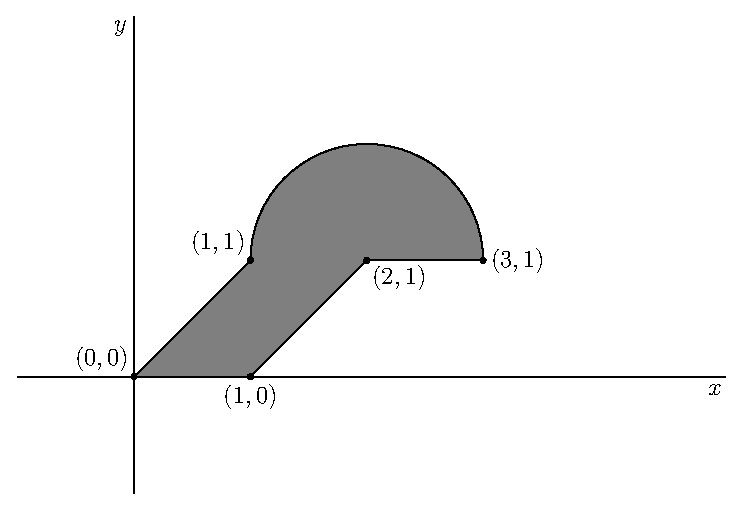
\includegraphics[width=10cm]{figure01.eps}
\caption{Region of Integration}
\label{figure-integral-example}
\end{figure} 
\newpage

\begin{example}
Say we wanted to integrate the function $f(x,y) = xy$ over the
triangle $T$ with vertices $(0,0)$, $(4,5)$ and $(6,2)$.
There isn't any one system of iterated integrals that covers
this region; therefore we have to treat it as two sections.
We divide the triangle into two pieces using the line $x=4$.
On the left, the $y$ coordinate is bounded by the lines
$y=x/3$ and $y=5x/4$. On the right, the $y$ coordinate is
bounded by $y=x/3$ and $y=-3x/2 + 11$. We calculate two
integrals.
\begin{align*}
\int_0^4 \int_{\frac{x}{3}}^{\frac{5x}{4}} xy dy dx & =
\int_0^4 \left. \frac{xy^2}{2}
\right|_{\frac{x}{3}}^{\frac{5x}{4}} dx \\
& = \int_0^4 \frac{x}{2} \left( \frac{25x^2}{16} -
\frac{x^2}{9} \right) dx \\
& = \int_0^4 \frac{25x^3}{32} - \frac{x^3}{18} = \int_0^4
\frac{209}{289} x^3 dx \\
& = \left. \frac{209}{288} \frac{x^4}{4} \right|_0^4 =
\frac{1196}{9} \\
\int_4^6 \int_{\frac{x}{3}}^{\frac{-3x}{2} - 11} xy dy dx & =
\int_4^6 \left. \frac{xy^2}{2}
\right|_{\frac{x}{3}}^{\frac{-3x}{2} - 11} dx \\
& = \int_4^6 \frac{x}{2} \left( \frac{-3x}{2} + 11 \right)^2 -
\frac{x}{2} \frac{x^2}{9} dx \\
& = \int_4^6 \frac{x}{2} \left( \frac{9x^2}{4} - 32 x + 121
\right) - \frac{x^3}{18} dx \\
& = \int_4^6 \frac{77x^3}{81} - \frac{33x^2}{2} + \frac{121
x}{2} dx \\
& = \left. \frac{77x^4}{324} - \frac{11x^3}{2} + \frac{121
x^2}{4} \right|_4^6 \\
& = \frac{77 \cdot 6^4}{324} - \frac{11 \cdot 6^3}{2} +
\frac{121 \cdot 6^2}{4} - \frac{77\cdot 4^4}{324} + \frac{11
4^3}{2} - \frac{121 \cdot 4^2}{4} = \frac{86845}{81}
\end{align*}
The total is the sum of the two integrals.
\begin{equation*}
\int_T f dA = \frac{1196}{9} + \frac{86845}{81} = \frac{97609}{81}
\end{equation*}
\end{example}

\begin{example}
Say we want to integrate the function $f(x) = x^2 + y^2$ over
the region shown in Figure \ref{figure-integral-example}.

We should divide the figure up into three pieces. The first
piece is the triangle $(0,0)$, $(1,1)$, and $(1,0)$. The
second is the half-circle above $y=1$. The third is the
remaining triangle $(1,1)$, $(2,1)$ and $(1,0)$.

The first integral is a short calculation.
\begin{align*}
\int_0^1 \int_0^x x^2 + y^2 dy dx & = \int_0^1 \left. x^2y +
\frac{y^3}{3} \right|_0^x \\
& = \int_0^1 \frac{4x^3}{3} = \left. \frac{x^4}{3} \right|_0^1
= \frac{1}{3} 
\end{align*}
The second integral is more involved. 
\begin{align*}
& \phantom{=} \int_1^3 \int_1^{1+\sqrt{1-(x-2)^2}} x^2 + y^2
dy dx \\
& =
\int_1^3 \left. x^2y + \frac{y^3}{3}
\right|_1^{1+\sqrt{1-(x-2)^2}} \\
& = \int_1^3 x^2 (1 + \sqrt{1-(x-2)^2}) +
\frac{(1+\sqrt{1-(x-2)^2})^3}{3} dx \\
u & = x-2 \\
& = \int_{-1}^1 (u^2 + 4u + 4) (1 + \sqrt{1-u^2}) + \frac{(1 +
\sqrt{1-u^2})^3}{3} du \\
& = \int_{-1}^1 u^2 + 4u + 4 + u^2 \sqrt{1-u^2} + 4u
\sqrt{1-u^2} + 4 \sqrt{1-u^2} \\
& \hspace{1cm} + \frac{1}{3} + \sqrt{1-u^2} +
(1-u^2) - \frac{u^2}{3} \sqrt{1-u^3} du \\
&= \int_{-1}^1 \frac{16}{3} + 4u + 5 \sqrt{1-u^2} +
4u \sqrt{1-u^2} + u^2 \sqrt{1-u^2} + \frac{1}{3}
(1-u^2)^{\frac{3}{2}} du \\
& = \frac{16u}{3} + 2u^2 + \left. 4 (1-u^2)^\frac{3}{2}
\frac{-2}{3} \right|_{-1}^1 + 5 \int_{-1}{1} \sqrt{1-u^2} du +
\int_{-1}^1 u^2 \sqrt{1-u^2} du + \frac{1}{3} \int_{-1}^1
(1-u^2)^{\frac{3}{2}} du \\
& = \frac{32}{5} + 0 + 0 + \left. \frac{1}{8} 2
\sqrt{1-u^2}(2u^2-1) + \arcsin u \right|_{-1}^1 + \left. 5 (u
\sqrt{1-u^2} + \arcsin u) \right|_{-1}^1 \\
& \hspace{1cm} + \left. \frac{1}{3}
\frac{1}{8} (u(5-2u^2)\sqrt{1-u^2} + 3 \arcsin u )
\right|_{-1}^1 \\
& = \frac{32}{3} + \frac{1}{8} \left( \frac{\pi}{2} -
\frac{-\pi}{2} \right) + 5 \left( \frac{\pi}{2} -
\frac{-\pi}{2} \right) + \frac{1}{8} \left( \frac{\pi}{2} -
\frac{-\pi}{2} \right) \\
& = \frac{32}{3} + \frac{\pi}{8} + 5\pi + \frac{\pi}{8} =
\frac{32}{3} + \frac{21\pi}{4} 
\end{align*}
The third integral is not quite as bad as the second.
\begin{align*}
\int_1^2 \int_{x-1}^1 x^2 + y^2 dy dx & = \int_1^2 \left. x^2 y +
\frac{y^3}{3} \right|_{x-1}^1 dx \\
& = \int_1^2 x^2 + \frac{1}{3} - x^2(x-1) - \frac{1}{3}
(x-1)^3 dx \\
& = \int_1^2 \frac{2}{3} - x + 3x^2 - \frac{4x^3}{3} dx \\
& = \left. \frac{2x}{3} - \frac{x^2}{2} + x^3 - \frac{x^4}{3}
\right|_1^2 \\
& = \frac{4}{3} - 2 + 8 - \frac{16}{3} - \frac{2}{3} +
\frac{1}{2} - 1 + \frac{1}{3} \\
& = \frac{7}{6} 
\end{align*}
The total is the sum of the three integrals.
\begin{equation*}
\frac{1}{3} + \frac{32}{3} + \frac{21\pi}{4} + \frac{7}{6} =
\frac{73}{6} + \frac{21\pi}{4} 
\end{equation*}
\end{example}

\begin{example}
Here is an odd application of multiple integration. We know
that $e^{-x^2}$ has no elementary antiderivative. Therefore,
the intergal
\begin{equation*}
A = \int_{-\infty}^\infty e^{-x^2} dx 
\end{equation*}
cannot be evaluated directly. However, this is a very
important integral: $e^{-x^2}$ is the 
normal distribution and, in Statistics, we need to integrate 
it frequently. We'll use
integrals over $\RR^2$, strangely enough, to calculate this
integral by squaring the single variable integra.
\begin{align*}
A & = 2 \int_{0}^\infty e^{-x^2} dx \\
A^2 & = \left( 2 \int_{0}^\infty e^{-x^2} dx \right) \left(2
\int_{0}^\infty e^{-y^2} dy \right) 
\end{align*}
The second integral uses a new variables since variables of
integration only matter inside the integral. Then we can
combine the two integrals.
\begin{align*}
A^2 & = 4 \int_0^\infty \int_0^\infty e^{-x^2} e^{-y^2} dx dy
\\
& = 4 \int_0^\infty \int_0^\infty e^{-(x^2 + y^2)} dx dy 
\end{align*}
\newpage

Now we are going to do a substitution in the $y$ variable.
Treating the $x$ variable as a constnat, we 
replace $y$ with $y = xs$ so that $dy = x ds$.
If $y=0$ then $s=0$ and as $y \rightarrow \infty$, $s
\rightarrow \infty$, so the bound for $s$ remain the same as
the bounds for $y$. Remember, $x$ is a constant through this
whole substitution. 
\begin{align*}
A^2 & = 4 \int_0^\infty \int_0^\infty -e^{-x^2 (1+s^2)} x dx ds
\\
& = 4 \int_0^\infty \left. \frac{-1}{2(1+s^2)} e^{-x^2(1+s^2)}
\right|_0^\infty ds \\
& = 2 \int_0^\infty \frac{1}{1+s^2} ds \\
& = \lim_{a \rightarrow \infty} 2 \arctan a - \arctan 0 =
\frac{2\pi}{2} = \pi \\
A & = \int_{-\infty}^\infty e^{-x^2} dx = \sqrt{\pi}
\end{align*}
We recover the area under the bell curve: $\sqrt{\pi}$. It's a
very strange result. However, if you taken any statistics and
worked on normal distributions, likely you will recall the
presence of these strange $\sqrt{\pi}$ terms. Now we know
they are present to normalize the area (since we want a
probability function to have area one under its graph).
\end{example}

\section{Change of Variables}
\label{change-of-variables}

Substitution was very useful for single variable integration.
In the $e^{-x^2}$ example, we did single-variable substitution
in $y$, treating $x$ as a constant. One might think that
since we do iterated integrals, single variable substitution
is sufficient. However, treating substitution in several
variables holistically turns out to be very useful and
powerful.

Let's review single variable substitution, formalizing the
language and showing the way forward for higher dimensions.
Consider a single variable integral.
\begin{equation*}
\int_{x=a}^{x=b} f(x) dx
\end{equation*}
Typically, we substitute $u = g(x)$ using some
\emph{invertible} function $g$. Then we have $du =
g^\prime(x) dx$ and we try to change all the $x$ variables to
$u$ variables with some algebra. We also change the bounds,
starting from $u = g(a)$ to $u = g(b)$. In this process, the
old variable is the \emph{domain} of the transformation and
the new variable is the \emph{range}.

However, for several variables we're going other direction.
We want the starting variables $x_i$ to be the range. We do
have one example from single variable calculus in this style;
trigonometric substitution, such as $x = a \sin \theta$, have
the original variable as the output of the transformation. 

Therefore, in the single variable case, introduce a new
variable $u$ by $x = h(u)$ for some \emph{invertible} function
$h$. Then $dx = h^\prime(u) du$ and the bounds become
$h^{-1}(a)$ and $h^{-1}(b)$. We get a new integral in the
variable $u$.

\begin{equation*}
\int_{u=h^{-1}(a)}^{u=h^{-1}(b)} f(h(u)) h^\prime(u) du 
\end{equation*}
The key relationship here is $dx = h^\prime(u) du$: the
derivative tells us the relationships between the differential
terms. In Calculus III, we did all that work on extending the
notion of the derivative. We came to the conclusion that the
derivative measures (in local coordinates) the best linear
approximation to the function. In one variable, that was just
multiplication by a number. In several variables, though,
that linear approximation was a matrix, called the Jacobian
matrix. Let's recall the definition. 

\begin{defn}
Let $F: \RR^n \rightarrow \RR^n$ be a function on $n$
variables, $x_1, \ldots, x_n$. We can write $F$ as its
component functions $F_1, \ldots, F_n$. Then the Jacobian
Matrix of $F$ is the matrix of all partial derivatives.
\begin{equation*}
J(F) = \left( \begin{matrix}
\frac{\del F_1}{\del x_1} & 
\frac{\del F_1}{\del x_2} & 
\ldots & 
\frac{\del F_1}{\del x_n} \\
\frac{\del F_2}{\del x_1} & 
\frac{\del F_2}{\del x_2} & 
\ldots & 
\frac{\del F_2}{\del x_n} \\
\vdots & \vdots & \vdots & \vdots \\
\frac{\del F_n}{\del x_1} & 
\frac{\del F_n}{\del x_2} & 
\ldots & 
\frac{\del F_n}{\del x_n} \end{matrix} \right) 
\end{equation*}
The determinant $\det J(F)$ is called the Jacobian of the
function and is often written $|J(F)|$. Note that the
notation $|\cdot|$ is a reminder to take a determinant; it is
\emph{not} an absolute value. The Jacobian is often
negative.
\end{defn}

From the single variable case $dx = h^\prime(u) du$, the
Jacobian is part of the new differential $du$. 
If we start with variables $x_1, x_2, \ldots, x_n$ and we have
a function $F: \RR^n \rightarrow \RR^n$ that has $x_i$ as it
output (the original variables are the range of the
transformation), we can write $x_1 = F_1(u_1,
\ldots, u_n)$, $x_2 = F_2(u_1, \ldots, u_n)$ up to $x_n =
F_n(u_1, \ldots, u_n)$. The Jacobian determines the
relationship between the differential in these variables.
\begin{equation*}
dx_1 dx_2 \ldots dx_n = |J(F)| du_1 du_2 \ldots du_n 
\end{equation*}
We can interpret the Jacobian as the change in
area/volume/hyper-volume due to the change in variables. Its
appearance in the integral makes sense with this
interpretation: the integral is measureing
area/volume/hyper-volume, so when we change variables, we need
a term that keeps track of the relative change in
area/volume/hypervolume.

\begin{example}
 Let $(x,y) = F(u,v) = (3u, 4v)$. Then we have
\begin{align*}
\frac{\del F_1}{\del u} & = 3 \\
\frac{\del F_1}{\del v} & = 0 \\
\frac{\del F_2}{\del u} & = 0 \\
\frac{\del F_2}{\del v} & = 4 \\
J(F) & = \left( \begin{matrix} 3 & 0 \\ 0 & 5 \end{matrix}
\right) \\
|J(F)| & = (3)(4) - (0)(0) = 12 \\
dx dy & = 12 du dv 
\end{align*}
The function is a dialation by $3$ in $u$ and by $4$ in $v$,
so the effect on area is multiplication by $12$, which makes
sense. The function is linear already, to the linear
approximation is constant: it is exactly the function itself.
\end{example}

\begin{example}
Let $(x,y) = F(u,v) = (u^2, v)$.
\begin{align*}
\frac{\del F_1}{\del u} & = 2u \\
\frac{\del F_1}{\del v} & = 0 \\
\frac{\del F_2}{\del u} & = 0 \\
\frac{\del F_2}{\del v} & = 1 \\
J(F) & = \left( \begin{matrix} 2u & 0 \\ 0 & 1 
\end{matrix} \right) \\
|J(F)| & = 2u \\
dx dy & = 2u du dv
\end{align*} 
This Jacobian isn't constant. This is a stretch in $u$, the
but effect is exagerated away from the origin due to the
square term. Therefore, as $u$ get larger, the stretch effect
is greater. The Jacobian reflects that.
\end{example}

\begin{example}
Let $(x,y) = F(r,\theta) = (r \cos \theta, r \sin \theta)$.
(Polar coordinates!)
\begin{align*}
\frac{\del F_1}{\del r} & = \cos \theta \\
\frac{\del F_1}{\del \theta} & = -r\sin \theta \\
\frac{\del F_2}{\del r} & = \sin \theta \\
\frac{\del F_2}{\del \theta} & = r \cos \theta \\
J(F) & = \left( \begin{matrix} \cos \theta & - r \sin \theta
\\ \sin \theta & r \cos \theta \end{matrix} \right) \\
|J(F)| & = r \\
dx dy & = r dr d\theta
\end{align*} 
This Jacobian shows that the radius term gives the effect on
area. This make sense: for larger circles, the differential
area is part of a larger arc.
\end{example}

\begin{example}
Let $(x,y) = F(u,v) = (u, uv)$. This is the change in variables we
used in the $e^{-x^2}$ example, now treated as a two-variable
changes of variables.
\begin{align*}
\frac{\del F_1}{\del u} & = 1 \\
\frac{\del F_1}{\del v} & = 0 \\
\frac{\del F_2}{\del u} & = v \\
\frac{\del F_2}{\del v} & = u \\
J(F) & = \left( \begin{matrix} 1 & 0 \\ v & u
\end{matrix} \right) \\
|J(F)| & = u \\
dx dy & = u du dv
\end{align*} 
\end{example}

We can use a change of variables to help us with either the
integrand or the region of integration. Sometime, as in the following
examples, the same transformation helps both. When we are
choosing a change of variables to simplify the region of
integration, we are looking for a transformation where some of
the bounding curves of the region become $u=c$ or $v=c$. We
need constant bounds in at least one of the variable to set up
the iterated integral.

\begin{example}
Let $D$ be the region in the first quadrant between the lines
$x+y = 1$ and the line $x+y =2$. In the following integral,
we want to simply the integrand and integrate over a simpler
region if possible.
\begin{equation*}
\int_D \cos \left( \frac{y-x}{y+x} \right) dA
\end{equation*}
To simplify the integrand, we can look for transformations
where $u = x+y$ and $v = x-y$. Inverting these (either by
linear algebra, since the transformation is linear, or just by
solving with conventional algebra), we get $x = \frac{u+v}{2}$
and $y = \frac{u-v}{2}$. 

Then we look at the bounds. If we take $x+y=1$ and replace $x$
and $y$, we get $u=1$. Likewise, $x+y=2$ is $u=2$. This is
excellent, since we need at least one variable with constant
bounds; we'll take $u$ to be the variable of the outside
integral. The other bounds are the axes, which we can express
by the equations $y=0$ and $x=0$. These turn into $u=v$ and
$u=-v$, respective. Therefore, the bounds of $v$ will be these
two lines: $v \in [u, -u]$.

Finally, we calculate the Jacobian.
\begin{align*}
x_u & = \frac{1}{2} \\
x_v & = \frac{1}{2} \\
y_u & = \frac{1}{2} \\
y_v & = -\frac{1}{2} \\
|J| & = -\frac{1}{2} \\
dx dy & = \frac{1}{-2} du dv
\end{align*}
We have the new integrand, the new bounds and the Jacobian. We
can proceed to the new integral.
\begin{align*}
\int_D \cos \left( \frac{y-x}{y+x} \right) dA & = \int_1^2 \int_{-u}^u
\cos \left( \frac{-v}{u} \right) \frac{-1}{2} dv du \\
& = \frac{-1}{2} \int_1^2 \left. -\sin \left( \frac{-v}{u} \right)
(-u) \right|_{-u}^{u} du \\
& = \frac{-1}{2} \int_1^2 u (\sin (-1) - \sin(1)) du \\
& = \frac{\sin (1) - \sin (-1)}{2} \left. \frac{u^2}{2}
\right|_1^2 \\
& = \frac{\sin (1) - \sin (-1)}{2} (2 - \frac{1}{2}) =
\frac{3(\sin(1) - \sin(-1))}{4} 
\end{align*}
\end{example}

\begin{example} 
Let $D$ be the region in the plane bounded by the curves $y =
\frac{1}{x}$, $y = \frac{3}{x}$, $y = 3x$ and $y = x$.
Consider the following integral.
\begin{equation*}
\int_D xy dA
\end{equation*}
\newpage

The integrand is reasonable, so we will chose a substitution
to changes the bounds. We want constant bounds in at least one
variables. Here is one changes of variables which gets those
constant bound: $(x,y) = F(u,v) = (uv,v)$. The lines $y=3x$
and $y=x$ become $v=3uv$ and $v=uv$. Away from $v=0$, these
lines are $u=\frac{1}{3}$ and $u=1$, so we have constant
bounds in $u$ and we will treat $u$ as the outside variable.
(We are save with the assumption $v=0$ since $v=y$ and the
region is disjoint from the $x$-axis, where $y=0$).
The curves $y = \frac{1}{x}$ and $y = \frac{3}{x}$ become $v =
\frac{1}{uv}$ and $v = \frac{3}{uv}$, which simplify into
$uv^2 =1$ and $uv^2=3$. If we solve for $v$ we get $v =
\sqrt{\frac{1}{u}}$ and $v = \sqrt{\frac{3}{u}}$. That means
we can take $u \in [\frac{1}{3}, 3]$ and $v \in
\left[\sqrt{\frac{1}{u}}, \sqrt{\frac{3}{u}} \right]$. The
integrand $xy$ becomes $uv^2$.
\begin{align*}
x_u & = v \\
x_v & = u \\
y_u & = 0 \\
y_v & = 1 \\
|J| & = (v)(1) - (u)(0) = v \\
dx dy & = v du dv 
\end{align*}
Then we complete the change of variables.
\begin{align*}
\int_D xy dA & = \int_{\frac{1}{3}}^1
\int_{\sqrt{\frac{1}{u}}}^{\sqrt{\frac{3}{u}}} uv^2 v dv du \\
& = \int_{\frac{1}{3}}^1 \left. u\frac{v^4}{4}
\right|_{\sqrt{\frac{1}{u}}}^{\sqrt{\frac{3}{u}}} du \\
& = \int_{\frac{1}{3}}^1 \frac{u}{4} (\frac{9}{u^2} -
\frac{1}{u^2}) du \\
& = \int_{\frac{1}{3}}^1 \frac{-2}{u} du \\
& = 2 \ln |u| \bigg|_{\frac{1}{3}}^1 \\
& = 2 \ln 1 - 2 \ln \frac{1}{3} = -2 \ln \frac{1}{3} = 2 \ln 3 
\end{align*}
\newpage

For the same integral, we could have taken $y=v$ and $x=
\frac{u}{v}$. Under this transformation, the bounds become $u
\in [1,3]$ and $v \in [\sqrt{u}, \sqrt{3u}]$. The Jacobian is
now $\frac{1}{v}$ and the integrand is $u$.
\begin{align*}
\int_D xy dA & = \int_1^3 \int_{\sqrt{u}}^{\sqrt{3u}}
\frac{1}{v} u dv du \\
& = \int_1^3 u \ln |v| \bigg|_{\sqrt{u}}^{\sqrt{3u}}
du \\
& = \int_1^3 u (\ln |\sqrt{3u}| - \ln |\sqrt{u}|du \\
& = \int_1^3 \frac{1}{2} (u \ln 3u - u \ln u) du \\
& = \left. \frac{1}{2} \left(\frac{1}{4} u^2 (2 \ln 3u - 1)
\frac{1}{3} - \frac{1}{4} u^2 (2 \ln u - 1) \right) \right|_1^3 
\end{align*}
If we evaluate this, it will evaluate, eventually, to $2 \ln
3$. However, the result is obviously more complicated.
Different changes of variables can have very different effects
on the integral; some will make it easier, some more
difficult. Also, the answers from different change of
variables can look quite differet, such as the expression
above, while actually being the same value.

As an aside, there is a simplification in the second version
of this example that removes the complication. In the second
last step, we could write $\ln 3u$ as $\ln 3 + \ln u$. 
\begin{align*}
& = \int_1^3 \frac{1}{2} (u \ln 3u - u \ln u) du \\
& = \frac{1}{2} \int_1^3 u (\ln 3 + \ln u - \ln u) du =
\frac{1}{2} \int_1^3 u \ln 3 du \\
& = \left. \frac{\ln 3}{2} \frac{u^2}{2} \right|_1^3 =
\frac{\ln 3}{4} (9-1) = \frac{8 \ln 3}{4} = 2 \ln 3
\end{align*}
\end{example}

\begin{example}
\begin{align*}
\int_I f(x,y) dA & = \int_0^2 \int_3^6 \frac{3x+y}{2x-y} dy dx
\\
x & = \frac{u+v}{5} \\
y & = \frac{2u-3v}{5} \\
J & = \left( \begin{matrix} \frac{1}{5} & \frac{1}{5} \\
\frac{2}{5} & \frac{-3}{5} \end{matrix}
\right) \\
|J| & = \frac{-1}{5} \\
dy dx & = \frac{-1}{5} du dv \\
\frac{3x+y}{2x-y} & = \frac{3u+3v+2u -3v}{2u + 2v -2u + 3v} =
\frac{5u}{5v} = \frac{u}{v} 
\end{align*}
The change of variables does indeed simplify the integrand,
but what about the region of integration? We know $(x,y) \in
[0,2] \times [3,6]$. Looking at the boundary lines$x=0$ and
$x=2$ in the changes of variables gives $u+v=0$ and $u+v-10$.
Likewise, $y=3$ and $y=6$ give $2u-3v=15$ and $2u-3v=30$. The
resulting shape is a parallelogram with vertices $(9,1)$,
$(12,-2)$, $(6,-6)$ and $(3,-3)$. We would have to split up
the domain of integration into three pieces to evaluate this;
the result may be a much longer process than dealing with the
original integral. Substitution may not always make things
easier.
\end{example}

\section{Polar Coordinates}
\label{polar-coordinates}

We often use substitution in several variables to simplify the
domain of integration instead of simplifying the function.
Polar coordinates are ideals for a domain of integration which
 has any kind of circular symmetry: circles, wedges, arcs,
etc.

The polar coordinate transformation is $x = r \cos \theta$ and
$y = r \sin \theta$ with Jacobian $|J| = r $ so that $dx dy =
r dr d\theta$. (Notice this Jacobian also corrects units: $dx
dy$ has units of length squared, but $\theta$ doesn't have any
units, so $r dr d\theta$ also has units of length squared.)

First, we need to understand what happens with constant bounds
in polar coordinates. If $r \in [0,R]$ and $\theta \in [0,
2\pi]$, we integrate over a whole circle of radius $R$.
Integrating over a wedge with radius $R$ from $\theta_1$ to
$\theta_2$ is $r \in [0,R]$ and $\theta \in [\theta_1,
\theta_2]$. Integrating over an annulus with radii $R_1$ and
$R_2$ is $r \in [R_1, R_2]$ and $\theta \in [0, 2\pi]$.
Finally, over an arc in such an annulus is $r \in [R_1, R_2]$
and $\theta \in [\theta_1, \theta_2]$.

\begin{example}
Consider the function $f(x,y) = x + y$ on the
arc in the first quadrant between radii $2$ and $4$. 
\begin{align*}
\int_D x + y dA & = \int_0^{\pi/2} \int_2^4 r (\cos \theta +
\sin \theta) r dr d\theta \\
& = \int_0^{\pi/2} \left. \frac{r^3}{r} (\cos \theta + \sin
\theta) \right|_2^4 d\theta \\
& = \frac{56}{3} \int_0^{\pi/2} (\cos \theta + \sin \theta) d
\theta \\
& = \left. \frac{56}{3} (\sin \theta - \cos \theta)
\right|_0^{\pi/2} \\
& = \frac{56}{3} (1 - 0 - 0 + 1) = \frac{112}{3} 
\end{align*}
\end{example}

\begin{example}
Now consider the function $e^{x^2 + y^2}$ on the circle of
radius $R$ centered at the origin. Notice here that the
integrand also has circular symmetry -- changing to polar
coordinates will help the integrand as well as the domain.

The integral is annoying in conventional Cartesian
coordinates.
\begin{equation*}
\int_D f(x,y) dA = \int_{-R}^R \int_{-\sqrt{R^2 -
x^2}}^{\sqrt{R^2 - x^2}} e^{x^2 + y^2} dy dx
\end{equation*}
This is essentially impossible. However, in polar coordinates
it improves greatly.
\begin{align*}
\int_D f(x,y) dA & = \int_0^{2\pi} \int_0^R e^{r^2} r dr
d\theta \\
& = \int_0^{2\pi} d\theta \int_0^R e^{r^2} r dr \\
& = 2\pi \left. \frac{e^{r^2}}{2} \right|_0^R = \frac{2\pi}{2}
(e^{R^2} - 1) = \pi (e^{R^2} - 1)
\end{align*}
\end{example}

\begin{example}
Now recall the integral we did to calcluate the volume of a
sphere of radius $R$.
\begin{equation*}
8 \int_0^{R} \int_0^{R^2 - x^2} \sqrt{R^2 - x^2 - y^2} dy dx 
\end{equation*}
This was a trickly integral. If we change to polar
coordinates, an integrate over the whole circle instead of
just a quarter, the integral improves.
\begin{align*}
A & = 2 \int_0^{2\pi} \int_0^R \sqrt{R^2 - r^2} r dr d\theta \\
& = 2 \int_0^{2\pi} d\theta \int_0^R \sqrt{R^2 - r^2} r dr
d\theta \\
& = 4\pi \left. (R^2 - r^2)^{\frac{3}{2}} \frac{2}{3}
\frac{-1}{2} \right|_0^R \\
& = \frac{4\pi}{3} (R^2)^{\frac{3}{2}} = \frac{4\pi R^3}{3}
\end{align*}
\end{example}

\begin{example}
For the cone of height
$h$ and radius $R$, we had the following integral.
\begin{equation*}
\int_D f(x,y) dA = 4 \int_0^r \int_0^{\sqrt{r^2 - x^2}} \left(
h - \frac{h}{r} \sqrt{x^2 + y^2} \right) dy dx
\end{equation*}
We didn't even evaluate the cone volume integral before, but
now we can use polar coordinates to make it much more
accessible.
\begin{align*}
A & = \int_0^{2\pi} \int_0^R \left( h - \frac{hr}{R} \right) r
dr d\theta \\
& = 2\pi \left. \left( \frac{hr^2}{2} - \frac{hr^3}{3R} \right)
\right|_0^R \\
& = 2\pi \left( \frac{hR^2}{2} - \frac{hR^2}{3} \right) =
\frac{\pi R^2 h}{3}
\end{align*}
\end{example}

\begin{example}
To show how some of these techniques work together, consider
integrating the function $f(x,y) = x^2$ over the ellipse
$D = \frac{x^2}{4} + \frac{y^2}{9} = 1$.
\begin{equation*}
\int_D x^2 dA 
\end{equation*}
We're going to do two changes of variables. First we can take
$x=2u$ and $y=3v$. That has Jacobian $|J| = 6$ so that $dx dy
= 6 du dv$. The ellipse $D$ becomes the unit circle $C$.
\begin{equation*}
\int_C (2u)^2 6 du dv = 24 \int_C u^2 du dv 
\end{equation*}
Then we change to polar coordinates to integrate over this
circle.
\begin{align*}
24 \int_C u^2 du dv & = 24 \int_0^{2\pi} \int_0^1 r^2 \cos^2
\theta r dr d\theta \\
& = 24 \int_0^{2\pi} \cos^2 \theta d \theta \int_0^1 r^3 dr \\
& = 24 \left. \left( \frac{\theta}{2} + \frac{\sin 2\theta}{4}
\right) \right|_0^{2\pi} \left. \left( \frac{r^4}{4} \right)
\right|_0^1 \\
& = 24 \pi \frac{1}{4} = 6 \pi 
\end{align*}
\end{example}

\begin{example}
Say we wanted to integrate the function $x^2 + y^2$
over the circle of radius 1 centered at $(1,0)$. The
integrand obviously lends itself to polar coordinates. There
is circular symmetry in the domain, but the offset is
confusing.

The equation of such a circle is $(x-1)^2 + y^2 = 1$. In
polar coordinates this is $r^2 \cos^2 \theta - 2 r \cos
\theta + 1 + r^2 \sin^2 \theta =1$, which simplifies into $r^2
- 2r \cos \theta = 0$ or $r = 2 \cos \theta$ for $\theta \in
[-\pi/2, \pi/2]$. We can take a constant bound for $\theta$
and have $\theta$ be the outside variable. Then we can use the
expression $r = 2 \cos \theta$ as an higher bound for $r$ in
terms of $\theta$.
\begin{align*}
\int_D f(x,y) dA & = \int_{-\pi/2}^{\pi/2} \int_0^{2\cos
\theta} \frac{1}{r^2} r dr d\theta \\
& = \int_{-\pi/2}^{\pi/2} \left. \frac{r^4}{4} \right|_0^{2
\cos \theta} d \theta \\
& = 4 \int_{-\pi/2}^{\pi/2} \cos^4 \theta d \theta \\
& = 4 \left. \frac{1}{32} \left( 12 \theta + 8 \sin (2\theta) +
\sin (4\theta) \right) \right|_{-\pi/2}^{\pi/2} \\
& = \frac{1}{8} \left(12 \left( \frac{\pi}{2} - \frac{-\pi}{2}
\right) \right) + 0 + 0 = \frac{3\pi}{2} 
\end{align*}
\end{example}

\begin{example}
What if $D$ is the circle of radius $2$ excluding the circle
of radius $1$ centered at $(1,0)$ and we want to integrate
$\sqrt{x^2 + y^2}$ over this region? Here, we can think of
the entire circle of radius 2 as $D_1$ and the removed circle
as $D_2$; then the integral will be the integral over $D_1$
subtracting the integral over $D_2$. 

The first part is an integral over $D_1$.
\begin{align*}
\int_{D_1} \sqrt{x^2 + y^2} dA & = \int_0^{2\pi} \int_0^2 r r
dr d\theta \\
& = \left. 2\pi \frac{r^3}{3} \right|_0^2 = \frac{16\pi}{3}
\end{align*}
The second part is an integral over $D_2$.
\begin{align*}
\int_{D_2} \sqrt{x^2 + y^2} dA & =
\int_{\frac{-\pi}{2}}^{\frac{\pi}{2}} \int_0^{2 \cos \theta}
r^2 dr d\theta \\
& = \int_{\frac{-\pi}{2}}^{\frac{\pi}{2}} \left. \frac{r^3}{3}
\right|_0^{2 \cos \theta} d\theta \\
& = \int_{\frac{-\pi}{2}}^{\frac{\pi}{2}} \left( 
\frac{8 \cos^3 \theta}{3} \right) = 
\frac{8}{3} \int_{\frac{-\pi}{2}}^{\frac{\pi}{2}} \cos^3
\theta d \theta \\
& = \frac{8}{3} \left. \left( \frac{1}{3} (2 + \cos^2
+ \theta) \sin \theta \right)
\right|_{\frac{-\pi}{2}}^{\frac{\pi}{2}} = \frac{32}{9} 
\end{align*}
The result of the original integral is the difference of the
two parts.
\begin{equation*}
\int_{D_1 \backslash D_2} \sqrt{x^2 + y^2} dA = \frac{16\pi}{3} -
\frac{32}{9} = \frac{48\pi - 32}{9}
\end{equation*}
\end{example}

\section{Cylindrical and Spherical Coordinates}
\label{cylindrical-and-spherical}

\subsection{Cylindrical Coordinates}
\label{cylindrical}

Cylindrical coordinates leave $z$ unchanges and use polar
coordinates in the $xy$-plane.
\begin{align*}
x & = r \cos \theta \\
y & = r \sin \theta \\
z & = z
\end{align*}
The Jacobian is $J = r$, using a $3 \times 3$ determinant. We
look to use cylindrical coordinates whenever a region in
$\RR^3$ has some kind of cylindrical shape or symmetry.

\begin{example}
Say the region $D$ is defined by $x^2 + y^2 \leq 4$ and $1
\leq z \leq 5$. This is a cylinder of radius $2$ of height
$4$. Say we want to integrate the function $f(x,y,z) =
z\sqrt{x^2+y^2}$ over this cylinder.
\begin{align*}
\int_D z\sqrt{x^2+y^2} dV & = \int_0^{2\pi} \int_0^2 \int_1^5
z r r dz dr d\theta \\
& = \int_0^{2\pi} d\theta \int_0^2 r^2 dr \int_1^5 z dz \\
& = 2\pi \left. \frac{r^3}{3} \right|_0^2 \left. \frac{z^2}{2}
\right|_1^5 = 2\pi \frac{24}{2} \frac{8}{3} = 64\pi 
\end{align*}
\end{example}

\begin{example}
We could have set up the volume of a cone in cylindrical
coordinates. If the cone has height $h$ and base radius $R$,
and we set it opening upwards with its point at the origin,
then we have $z \in [0,h]$ and the radius increases linearly
with $z$ as $r = \frac{zR}{h}$. In $\RR^3$, we integrat $1$
over the cone to calculate its volume. The bounds for $z$ are
non-constant, so $z$ must be the inside variable.
\begin{align*}
\int_C 1 dV & = \int_0^{2\pi} \int_0^h \int_0^{\frac{Rz}{h}} r
dr dz d\theta \\
& = 2\pi \int_0^h \left. \frac{r^2}{2}
\right|_0^{\frac{Rz}{h}} dz \\
& = 2\pi \int_0^h \frac{R^2 z^2}{2h^2} dz \\
& = 2\pi \left. \frac{R^2}{2h^3} \frac{z^3}{3} \right|_0^h \\
& = 2\pi \frac{R^2}{2h^3} \frac{h^3}{3} = \frac{R^3h\pi}{3}
\end{align*}
\end{example}

\begin{example}
Similarly, we can calculate the volume of a parabaloid this
way. We orient it along the $z$ axis, opening upwards. If
the parabaloid has height $h$ and base radius $R$, then the
radius if $r = \frac{R\sqrt{z}}{\sqrt{h}}$. By solving for
$z$, we have $z = \frac{hr^2}{R^2}$. The bounds for $z$ are
non-constant, so $z$ must be the inside integral.
\begin{align*}
\int_D 1 dV & = \int_0^{2\pi} \int_0^R \int_{\frac{hr^2}{R^2}}^h
r dz dr d\theta \\
& = 2\pi \int_0^R r \left( h - \frac{hr^2}{R^2} \right) dr \\
& = 2\pi \left. \left( \frac{hr^2}{2} - \frac{hr^4}{4R^2}
\right) \right|_0^R \\
& = 2\pi \left( \frac{hR^2}{2} - \frac{hR^4}{4R^2} \right) \\
& = hR^2 2\pi \left( \frac{1}{2} - \frac{1}{4} \right) \\
& = \frac{hR^2 \pi}{2}
\end{align*}
\end{example}

\begin{example}
Assume we have three cylinders of radius $R$ along each axis
in $\RR^3$. What is the volume of the intersection of all
three cylinders? (This is called the tricylinder Steinmetz
solid). Setting up the geometry is difficult. We will
integrate and height over the $xy$ plane, and by symmetry, we
can work with one 16th of the shape: the portion that lies
above one 8th of the circle above the axis. In the first 8th
of the circle ($\theta \in [0, \pi/4]$) in polar coordinates).
The $z$-axis cylinder restricts us to the circle in the
$xy$-plane and the $x$-axis cylinder is lower than the
$y$-axis cylinder over this particular $8th$ or a circle, so
the $x$-axis cylinder is the limit on height. What is that
height function? The equation of the cylinder is $y^2 + z^2 =
R^2$, so we have $z ^2 = R^2 - y^2 = R^2 - r^2 \sin^2\theta$,
writing $y$ in cylindrical coordinates. This determines a region of
integration and we proceed using cylindrical coordinates.

\begin{align*}
V & = 16 \int_0^{\frac{\pi}{4}} \int_0^R \int_0^{\sqrt{R^2-r^2
\cos^2\theta}} r dz dr d\theta \\
& = 16 \int_0^{\frac{\pi}{4}} \int_0^R \sqrt{R^2-r^2
\cos^2\theta} r dr d\theta \\
& = 16 \int_0^{\frac{\pi}{4}} \left. \left( (R^2-r^2
\cos^2\theta)^{\frac{3}{2}} \frac{2}{3}
\frac{-1}{2\cos^2\theta} \right) \right|_0^R d\theta \\
& = \frac{16}{3} \int_0^{\frac{\pi}{4}} \left(
\frac{R^3}{\cos^2 \theta} - \frac{(R^2-R^2\cos^2
\theta)^{\frac{3}{2}}}{\cos^2 \theta} \right) d \theta \\
& = \frac{16}{3} \int_0^{\frac{\pi}{4}} \left(
R^3\sec^2 \theta - \frac{R^3\sin^3 \theta}{\cos^2 \theta} \right) d
\theta \\
& = \frac{16R^3}{3} \int_0^{\frac{\pi}{4}} \left(
\sec^2 \theta - \frac{\sin \theta}{\cos^2 \theta} + \sin
\theta \right) d \theta \\
& = \frac{16R^3}{3} \left. \left( \tan \theta + \frac{-1}{\cos
\theta} - \cos \theta \right) \right|_0^{\frac{\pi}{4}} \\
& = \frac{16R^3}{3} \left( 1 - \frac{2}{\sqrt{2}} -
\frac{\sqrt{2}}{2} - 0 + 1 + 1 \right) \\
& = \frac{16R^3}{3} \left( 3 - \frac{2\sqrt{2} + \sqrt{2}}{2} =
\frac{16R^3}{3} \frac{6-3\sqrt{2}}{2} \right) = 8R^3 (2-\sqrt{2})
\end{align*}
\end{example}

\subsection{Spherical Coordinates}
\label{spherical}

Spherical coordinates use a spherical radius and two angles:
$\phi$ as co-latittude and $\theta$ as longitude. The ranges
for the angles are $\phi \in [0,\pi]$ and $\theta \in [0,
2\pi]$. 
\begin{align*}
x & = r \sin \phi \cos \theta \\
y & = r \sin \phi \sin \theta \\
z & = r \cos \phi
\end{align*}
The Jacobian is $J = r^2 \sin \phi$, after a complicated $3
\times 3$ determinant. We use spherical coordinates when the
domain of integration has some kind of spherical shape or
symmetry.

\begin{example}
The easiest example is the volume of a sphere of radius $R$.
\begin{align*}
\int_S 1 dV & = \int_0^{2\pi} \int_0^{\pi} \int_0^R r^2 \sin
\phi dr d\phi d\theta \\
& = \int_0^{2\pi} d\theta \int_0^{\pi} \sin \phi d \phi
\int_0^R r^2 dr \\
& = 2\pi \left. \left( -\cos \phi \right) \right|_0^{\pi} \left.
\frac{r^3}{3} \right|_0^R \\
& = 2\pi ( 1+1) \frac{R^3}{3} = \frac{4\pi R^3}{3}
\end{align*}
\end{example}

\begin{example}
We can also calculate the volume of an eplipsoid.
\begin{equation*}
\frac{x^2}{a^2} + \frac{y^2}{b^2} + \frac{z^2}{c^2} = 1 
\end{equation*}
We use a linear change of variables first:$x =au$, $y = vb$ and $z=cw$
The Jacobian is $J = abc$ and the ellipsoid $E$ because a unit
sphere $S$.
\begin{equation*}
\int_E 1 dx dy dz = \int_S abc dudvdw
\end{equation*}
Then, since $a$, $b$ and $c$ are constant, this just the
volume of a sphere of radius 1.
\begin{equation*}
\int_E 1 dx dy dz = \int_S abc dudvdw = abc \int_S 1 du dv
dw = \frac{4\pi abc}{3}
\end{equation*}
\end{example}

\begin{example}
Consider a sphere of radius $R$. Inside this sphere is a cone
with flare angle $\pi/6$, where the tip of the cone is located
at very bottom of the sphere and the cone opens up inside the
sphere. The cone, plus the portion of the sphere above the
cone, gives a shape that is something like an ice-cream cone;
it's a cone plus a spherically curved cap at the top of the
cone. What is the volume of this object?

If we put the centre of the sphere at $(0,0,R)$, then the
vertex of the cone can be put at the origin. The equation of
such a sphere is
\begin{equation*}
x^2+ y^2 + (z-R)^2 = R^2.
\end{equation*}
Since $r^2 = x^2 + y^2 + z^2$, this equation simplifies into
$r^2 = 2 R z$ which is $r^2 = 2Rr\cos \phi$ or $r = 2R\cos
\phi$. This can be taken at the outside bound of the radius
term, as $\phi \in [0,\pi/2]$ and $\theta \in [0, 2\pi]$. The
flare of the cone is $\pi/6$, which restricts $\phi \in [0,
\pi/6]$. We integrate with these bounds for the volume, making
sure that $r$ is an inside integral since its bounds depend on
$\theta$.

\begin{align*}
\int_D 1 dV & = \int_0^{2\pi} \int_0^{\frac{\pi}{6}} \int_0^{2
R \cos \phi} r^2 \sin \phi dr d\phi d\theta \\
& = 2\pi \int_0^{\frac{\pi}{6}} \left. \frac{r^3}{3}
\right|_0^{2R\cos \phi} \sin \phi d \phi \\
& = 2\pi \int_0^{\frac{\pi}{6}} \frac{8R^3 \cos^3 \phi \sin
\phi}{3} d\phi \\
& = \frac{16\pi r^3}{3} \left. \left( \frac{-\cos^4\phi}{4}
\right) \right|_0^{\frac{\pi}{6}} \\
& = \frac{16R^3\pi}{3} \left( \frac{1}{4} - \frac{9}{64}
\right) = \frac{7\pi R^3}{12}
\end{align*}
\end{example}

\section{Applications of Multiple Integration}
\label{applications}

We've already spoken about the general definition of the size
of sets, but let's remind ourselves. If $S$ is any integrable
set in $\RR^n$, then the size of $S$ is \emph{defined} to be
the integral of the constant function.
\begin{equation*}
V(S) = \int_S 1 dV
\end{equation*}
There are many physical problems involving 3D objets with
variable density where we desire to know mass instead of
volume. 
\begin{defn}
If $\rho(x,y,z)$ is a density function, integrable on a region
$S \in RR^3$, the mass of the object $S$ is found from
by integrating the density function.
\begin{equation*}
M(S) = \int_S \rho dV
\end{equation*}
This can also be done in $\RR^2$ for flat objects with variable
density depending on only $x$ and $y$. Such objects are
normally refered at laminae.
\end{defn}

A similar interesting physical problem is the problem of
centre of mass. The centre of mass of an rigid object (or
system) is the point in space where linear forces on the object can
be accuratly modeled as forces on a point-mass. In particular,
forces on the centre of mass do not cause rotational
acceleration. The calculation of centre of mass involves the
calculation of so-called first moments. These definition vary
by dimension. First we work with a lamina in $\RR^2$. 

\begin{defn}
Let $S$ be a region in $\RR^2$ with density $\rho(x,y)$. Its
\emph{mass} and \emph{first moments} are defined b the
following integrals.
\begin{align*}
m & = \int_S \rho dA \\
M_x & = \int_S y \rho dA \\
M_y & = \int_S x \rho dA \\
\end{align*}
Then the \emph{coordinates of the centre of mass} are written
$(\bar{x}, \bar{y})$ and calculate from the moments.
\begin{align*}
\bar{x} & = \frac{M_x}{m} \\
\bar{y} & = \frac{M_y}{m} \\
\end{align*}
If $S$ is a solid region in $\RR^3$ with density
$\rho(x,y,z)$, then its \emph{mass} and \emph{first moments}
are defined by the following integrals.
\begin{align*}
m & = \int_S \rho dV \\
M_{yz} & = \int_S x \rho dV \\
M_{xz} & = \int_S y \rho dV \\
M_{xy} & = \int_S z \rho dV \\
\end{align*}
The \emph{coordinates of the centre of mass} are written $(\bar{x},
\bar{y}, \bar{z})$ and calculated from the moment.
\begin{align*}
\bar{x} & = \frac{M_{yz}}{m} \\
\bar{y} & = \frac{M_{xz}}{m} \\
\bar{z} & = \frac{M_{xy}}{m} \\
\end{align*}
\end{defn}
\newpage

Centre of mass and first moments are important physical
properties that deal with linear acceleration; for the purpose
of linear acceleration, the object acts like a point mass at
the centre of mass. However, there are also moments involved
in rotational movement and acceleration. These are called
second moments or moments of intertia. 

Let $S \subset \RR^2$ be a laminae with density function
$\rho$. Its \emph{second moments} are calcaulted by the
following integrals.
\begin{align*}
I_x & = \int_S y^2 \rho dA \\
I_y & = \int_S x^2 \rho dA \\
I_0 & = \int_S (x^2+y^2) \rho dA 
\end{align*}
These moment measure the resistance to rotation: $I_x$ is the
resistance to rotation about the $x$ axis; $I_y$ is the
resistance to rotation about the $y$ axis; and $I_0$ is
resistance to rotation about the origin. The three \emph{radii
of gyration} are calcluated from the second moments.
\begin{align*}
\bar{\bar{R}}^2 & = \frac{I_0}{m} \\
\bar{\bar{x}}^2 & = \frac{I_x}{m} \\
\bar{\bar{y}}^2 & = \frac{I_y}{m} 
\end{align*}
The radii of gyration are similar to centre of mass for
movement. The object acts as a point mass at radius
$\bar{\bar{R}}$ for rotation about the origin. Similar, it
acts like a point mass at radius $\bar{\bar{x}}$ for rotation
about the $x$ axis and radius $\bar{\bar{y}}$ for rotation
about the $y$ axis.

Let $S$ be a solid object in $\RR^3$ with density function
$\rho$. Its \emph{second moments} are calculated by the
following integrals.
\begin{align*}
I_x & = \int_S (y^2 + z^2) dV \\
I_y & = \int_S (x^2 + z^2) dV \\
I_z & = \int_S (x^2 + y^2) dV 
\end{align*}
Its \emph{radii of gyration} are calculated from the second
moments.
\begin{align*}
\bar{\bar{x}}^2 & = \frac{I_x}{m} \\
\bar{\bar{y}}^2 & = \frac{I_y}{m} \\
\bar{\bar{z}}^2 & = \frac{I_z}{m} \\
\end{align*}
The object acts like a point mass at $(\bar{\bar{x}},
\bar{\bar{y}}, \bar{\bar{z}})$ for purposes of rotational
physics. More specifically, for about the $z$ axis, the
particular acts as a point mass at radius
$\sqrt{\bar{\bar{x}}^2 + \bar{\bar{y}}^2}$, with parallel
constructions for the other two axes.

\begin{example}
Consider a quarter circle of radius $a$ in the first quadrant
with density function $\rho = k\sqrt{x^2 + y^2}$. What is
its centre of mass?
\begin{align*}
m & = \int_0^{\frac{\pi}{2}} \int_0^a krrdr d\theta \\
& = \frac{\pi}{2} \left. \frac{kr^3}{3} \right|_0^a =
\frac{\pi ka^3}{6} \\
\bar{x} & = \frac{1}{m} \int_0^{\frac{\pi}{2}} \int_0^a y \rho
dA = \frac{1}{m} \int_0^{\frac{\pi}{2}} \int_0^a kr^3 \sin
\theta dr d\theta \\
& = \frac{k}{m} \int_0^{\frac{\pi}{2}} \sin \theta d\theta
\int_0^a r^3 dt \\
& = \frac{k}{m} \left. \left( -\cos \theta \right)
\right|_0^{\frac{\pi}{2}} \left. \frac{r^4}{4} \right|_0^a =
\frac{6}{\pi a^3} 1 \frac{a^4}{4} = \frac{3a}{2\pi}\\
\bar{y} & = \frac{3a}{2\pi}
\end{align*}
We don't have to calculate the second moment; $\bar{x} =
\bar{y}$ due to the symmetry of the situation. The centre of mass
is found at $\left( \frac{3a}{2\pi}, \frac{3a}{2\pi} \right)$. 
\end{example}

\begin{example}
Now consider a lamina with $y \in [-1,1]$ and $x$ bounded
between $\pm y^4$ with $\rho = 1$. What is the area and moment
of intertia about the $x$-axis?
\begin{align*}
A & = \int_{-1}^1 \int_{-y^4}^{y^4}1 dx dy \\
& = \int_{-1}^1 2y^4 dy = \left. \frac{2y^5}{5} \right|_{-1}^1
\\
& = \frac{4}{5} \\
I_x & = \int_{-1}^1 \int_{-y^4}^{y^4} y^2 dx dy \\
& = \int_{-1}^1 \left. xy^2 \right|_{-y^4}^{y^4} = \int_{-1}^1
2y^6 dy \\
& = \left. \frac{2y^7}{7} \right|_{-1}^1 = \frac{4}{7}
\end{align*}
Compare this lamina to a rectangle of height $2$ and width
$2/5$, which has the same area. We calculate the moment of
inertia for the rectangle.
\begin{equation*}
I_x = \int_{-1}^1 \int_{-\frac{1}{5}}^\frac{1}{5} y^2 dx dy =
\frac{4}{15}
\end{equation*}
Our shape has twice the resitance to rotation, even though it
has the same cross-section area. This physical fact 
partially explains the use of $I$ beams in construction: they
have more resistance to twisting and shear forces than a
rectangular cross-section beam of the same size or weight.
\end{example}

\begin{example}
Now consider a hemisphere above the $xy$ plane with radius
$a$ and density $\rho = kz$. Let's calculate its mass, centre
of mass, and moments of inertia.
\begin{align*}
m & = \int_0^{2\pi} \int_0^{\pi/2} \int_0^a k (r\cos \phi) r^2
\sin^2\phi dr d\phi d\theta \\
& = 2\pi k \int_0^{\pi/2} \left. \frac{r^4}{4} \right|_0^a
\cos \phi \sin \phi d\phi \\
& = \frac{2\pi ka^4}{4} \int_0^{\pi/2} \frac{\sin 2\phi}{2}
d\phi \\
& = \frac{\pi ka^4}{2} \left. \left( \frac{-\cos2\phi}{4}
\right) \right|_0^{\pi/2} = \frac{\pi ka^4}{8} ( \cos 0 - \cos
\pi) = \frac{\pi ka^4}{4} \\
M_{yz} & = 0 \text{ due to symmetry.} \\
M_{xz} & = 0 \text{ due to symmetry.} \\
M_{xy} & = \int_D z \rho dV \\
& = \int_0^{2\pi} \int_0^{\pi/2}
\int_0^a kr^2 \cos^2\phi r^2 \sin \phi dr d\phi d\theta \\
& = 2\pi k \int_0^a r^4 dr \int_0^{\pi/2} \cos^2 \phi \sin
\phi d \phi \\
& = \frac{2\pi k a^5}{5} \left. \left( \frac{-\cos^3 \phi}{3}
\right) \right|_0^{\pi/2} = \frac{2\pi k a^5}{15} \\
\bar{x} & = 0 \\
\bar{y} & = 0 \\
\bar{z} & = \frac{\frac{2\pi ka^5}{15}}{\frac{\pi ka^4}{4}} =
\frac{8a}{15} 
\end{align*}
The centre of mass is at $(0,0, \frac{8a}{15})$
Let's also calculate the moments of inertia.
\begin{align*}
I_x & = \int_D (y^2 + z^2) \rho dV = \int_D (y^2 + z^2) z k dV
\\
& = k \int_0^{2\pi} \int_0^{\pi/2} \int_0^a r^2 (\sin^2 \phi
\sin^2 \theta + \cos^2 \phi) r \cos \phi r^2 \sin\phi drd\phi
d\theta \\
& = k \int_0^a r^5 dr \int_0^{2\pi} \int_0^{\pi/2} \left(
\sin^3 \phi \cos \phi \sin^2 \theta + \cos^3 \phi \sin \phi
\right) d\phi d\theta \\
& = \frac{ka^6}{6} \left[ \left. \left( \frac{\sin^4 \phi}{4}
\right) \right|_0^{\pi/2} \left. \left( \frac{\theta}{2} -
\frac{\sin 2\theta}{4} \right) \right|_0^{2\pi} + \left.
\left( \frac{-\cos^4 \phi}{4} \right) \right|_0^{\pi/2} 2\pi 
\right] \\
& = \frac{ka^6}{6} \left[ \left( \frac{1}{4} - 0 \right) \pi _
2\pi \left( \frac{1}{4} - 0 \right) \right] = \frac{\pi
ka^6}{8} \\
I_y & = \frac{\pi ka^6}{8} \text{ by symmetry} \\
I_z & = \int_D (x^2 + y^2) \rho dV \\
& = k \int_0^{2\pi} \int_0^{\pi/2} \int_0^a r^2 \sin^2 \phi r
\cos \phi r^2 \sin \phi dr d\phi d\theta \\
& = \frac{2\pi ka^6}{6} \int_0^{\pi/2} \sin^3 \phi \cos \phi
d\phi \\
& = \frac{\pi ka^6}{3} \left. \frac{\sin^4 \phi}{4}
\right|_0^{\pi/2} = \frac{\pi ka^6}{12} \\
\bar{\bar{x}}^2 & = \frac{\frac{\pi ka^6}{8}}{\frac{\pi
ka^4}{4}} = \frac{a^2}{2} \\
\bar{\bar{x}} & = \frac{a}{\sqrt{2}} \\
\bar{\bar{y}}^2 & = \frac{a^2}{2} \\
\bar{\bar{y}} & = \frac{a}{\sqrt{2}} \\
\bar{\bar{z}}^2 & = \frac{\frac{\pi ka^6}{12}}{\frac{\pi
ka^4}{4}} = \frac{a^3}{3} \\
\bar{\bar{z}} & = \frac{a}{\sqrt{3}}
\end{align*}
The centre of rotation is at $\left( \frac{a}{\sqrt{2}},
\frac{a}{\sqrt{2}}, \frac{a}{\sqrt{3}} \right)$.
\end{example}
\newpage

\begin{example}
Now consider a parabaloid bounded by $z = b(x^2 + y^2)$ with
height $h$ and density $\rho = 1$. What are its moments of
inertia? We will use cylindrical coordinates, but we need a
bound on the radius term at the height $h$. The equation of
the parabaloid in cylindrical coordinates is $z = br^2$ and
when $z=h$, we see that $r = \sqrt{\frac{h}{b}}$. This is the
outer bound on radius. With contstant bounds on angle and
radius, we can let $z$ range from the parabaloid graph
$z=br^2$ to the constant height $h$.
\begin{align*}
m & = \int_R 1 dV = \frac{\pi \sqrt{\frac{h}{b}}^2h}{2} =
\frac{\pi h^2}{2b} \\
I_z & = \int_0^{2\pi} \int_0^{\sqrt{\frac{h}{b}}}
\int_{br^2}^h (x^2 + y^2) r dz dr d\theta \\
& = \int_0^{2\pi} \int_0^{\sqrt{\frac{h}{b}}} \int_{br^2}^h
r^3 dz dr d\theta \\
& = 2\pi \int_0^{\sqrt{\frac{h}{b}}} \left( r^3h - r^5 b \right) dr \\
& = 2\pi \left. \left( \frac{hr^4}{4} - \frac{br^6}{6}
\right) \right|_0^{\sqrt{\frac{h}{b}}} \\
& = 2\pi \left( \frac{h^3}{4b^2} - \frac{bh^3}{6b^3} \right)
= \frac{2\pi h^3}{b^2} \left( \frac{1}{4} - \frac{1}{6}
\right) = \frac{\pi h^3}{6b^2} \\
\bar{\bar{z}}^2 & = \frac{I_z}{m} = \frac{\frac{\pi
h^3}{6b^2}}{\frac{\pi h^2}{2b}} = \frac{h}{3b} \\
\bar{\bar{z}} & = \sqrt{\frac{h}{3b}}
\end{align*}

\begin{align*}
I_x & = \int_0^{2\pi} \int_0^{\sqrt{\frac{h}{b}}}
\int_{br^2}^h (y^2 + z^2) r dz dr d\theta \\
& = \int_0^{2\pi} \int_0^{\sqrt{\frac{h}{b}}} \int_{br^2}^h
(r^2 \sin^2 \theta + z^2) r dz dr d\theta \\
& = \int_0^{2\pi} \int_0^{\sqrt{\frac{h}{b}}} r^3 \sin^2 \theta \left( h-
br^2 \right) + r \left( \frac{h^3}{3} -
\frac{b^3r^6}{3}\right) dr d\theta \\
& = \int_0^{2\pi} \left. \frac{r^4}{4} h \sin^2 \theta -
\frac{r^6}{6} b \sin^2 \theta + \frac{r^2}{2}
\frac{h^3}{3} - \frac{r^8}{8} \frac{b^3}{3}
\right|_0^{\sqrt{\frac{h}{b}}} d \theta\\
& = \int_0^{2\pi} \frac{h^2}{4b^2} h \sin^2 \theta -
\frac{h^3}{6b^3} b \sin^2 \theta + \frac{h^4}{6b} - \frac{h^4
b^3}{24 b^4} d\theta \\
& = \frac{h^3}{b^2} \int_0^{2\pi} \sin^2 \theta d \theta \left(
\frac{1}{4} - \frac{1}{6} \right) + \frac{2\pi h^4}{b} \left(
\frac{1}{6} - \frac{1}{24} \right) \\
& = \left. \frac{h^3}{12b^2} \left( \frac{\theta}{2} -
\frac{\sin 2\theta}{4} \right) \right|_0^{2\pi} + \frac{3\pi
h^4}{12b} \\
& = \frac{h^3 \pi}{12b^2} + \frac{3\pi h^4}{12b} = \frac{h^3
\pi}{12b} \left( \frac{1}{b} + 3h \right) \\
\bar{\bar{x}}^2 & = \frac{ \frac{h^3\pi}{12b} \left(
\frac{1}{b} + 3h \right)}{\frac{\pi h^2}{2b}} \\
\bar{\bar{x}} & = \sqrt{\frac{a^2}{6} + \frac{h^2}{3}} =
\frac{h}{6} \left( \frac{1}{b} + 3h \right) \\
\bar{\bar{x}} & = \sqrt{\frac{h}{6} \left( \frac{1}{b} + 3h
\right)} \\
\bar{\bar{y}} & = \bar{\bar{x}} \text{ by symmetry} 
\end{align*}
\end{example}

As a final example for this section, we can prove a a nice theorem
from physics. 

\begin{thm}
A body of uniform density under the
action of a external conservative force (such a gravity) acts like
a point mass at its centre of mass. 
\end{thm}

\begin{proof}
We'll just prove the theorem for the special case of a sphere. 
The force of gravity between two masses $m_1$ and $m_2$ is
\begin{equation*}
F = \frac{Gm_1m_2}{r^2}
\end{equation*} 
Let's assume the source of the gravitational attraction sits
at $(0,0,c)$ where $c >a$ is larger than $a$ the radius of the
sphere. Let's also assume that $\rho$ is the constant density
of the sphere. Then $\rho dV$ is an infinitesimal piece of
mass in the sphere, and we can write $\omega$ for the distance
from the infinitesimal mass to the gravitational source.

The force on the infinitesimal mass is 
\begin{equation*}
F dV = \frac{Gm\rho dV}{\omega^2}.
\end{equation*}
In polar coordinates, this is 
\begin{equation*}
F dV = \frac{Gm\rho r^2 \sin \phi dr d\phi d\theta}{\omega^2}. 
\end{equation*}
By symmetry of the sphere, all lateral forces will cancel. We
only care about the $z$ component of the force. Let $\alpha$
be the angle from the $z$ axis of the line from $(0,0,c)$ to
the infinitesimal mass. 
\begin{equation*}
F_z dV = \frac{Gm\rho r^2 \sin \phi \cos \alpha dr d\phi
d\theta}{\omega^2} 
\end{equation*}
Let's do some trigonometry. Consider the triange with
vertices $(0,0,c)$, $(0,0,0)$ and the location of our
infinitesimal mass. The angle at $(0,0,c)$ is $\alpha$ by
definition, and likewise the angle at $(0,0,0)$ is $\phi$.
The side lengths are $c$, $\omega$ and $r$, also by
definition. We use the cosine law.
\begin{align*}
\omega^2 & = r^2 + c^2 - 2rc \cos \phi \\
\omega & = \sqrt{r^2 + c^2 - 2rc \cos \phi}
\end{align*}
The length $c$ along the $x$ axis can be divided into two
pieces, so that $c = \omega \cos \alpha + r \cos \phi$. We
can solve for $\cos \alpha$.
\begin{equation*}
\cos \alpha = \frac{ c - r \cos \phi}{\omega} 
\end{equation*}
We can replace $\omega$ with the square root expression.
\begin{equation*}
\cos \alpha = \frac{ c - r \cos \phi}{\sqrt{r^2 + c^2 - 2rc
\cos \phi}}
\end{equation*}
We can replace both $\cos \alpha$ and $\omega $in the force
expression.
\begin{equation*}
F_z dV = \frac{Gm\rho r^2 \sin \phi}{r^2 +
c^2 - 2rc\cos \phi} \left( \frac{c - r\cos \phi}{\sqrt{r^2 +
c^2 - 2rc \cos \phi}} \right) dr d\phi d\theta
\end{equation*}
The total force is this integral of this infinitesimal force
over the sphere.
\begin{equation*}
F_z = \int_0^{2\pi} \int_0^{\pi} \int_0^a \frac{Gm\rho r^2
\sin \phi}{r^2 + c^2 - 2rc\cos \phi} \left( \frac{c - r\cos
\phi}{\sqrt{r^2 + c^2 - 2rc \cos \phi}} \right) dr d\phi
d\theta
\end{equation*}
We'll do some substitution here, more or less reversing 
the trigonometry. We leave $r$ and $\theta$ along, but
write $\omega^2 = r^2 + c^2 - 2rc\cos\phi$ with the cosine law
as before.
\begin{equation*}
2\omega d\omega = 2rc \sin \phi d\phi \implies r \sin \phi
d\phi = \frac{\omega}{c} d\omega
\end{equation*}
We have $\omega(0) = c-r$ and $\omega(\pi) = c+r$ for the
bounds. Finally, we can solve to get $r\cos \phi = \frac{r^2 +
c^2 - \omega^2}{2c}$. We use this as a substitution in the
$\phi$ integral.
\begin{align*}
F_z & = \int_0^{2\pi} \int_0^{\pi} \int_0^a 
\frac{Gm\rho r}{(r^2 + c^2 - 2rc\cos \phi)} \frac{(c-r\cos
\phi)}{\sqrt{r^2+c^2-2rc\cos\phi}} (r\sin \phi d\phi) dr
d\theta \\
& = \int_0^{2\pi} \int_0^a \int_{c-r}^{c+r} \frac{Gm\rho
r}{\omega^2} \frac{c - \frac{r^2 + c^2 -
\omega^2}{2c}}{\omega} \frac{\omega}{c} d\omega dr d\theta \\
& = \int_0^{2\pi} \int_0^a \int_{c-r}^{c+r} \frac{Gm\rho
r}{\omega^2} \frac{2c^2 - r^2 - c^2 + \omega^2}{2c^2} \omega
dr d\theta \\
&= \frac{2\pi Gm \rho}{2c^2} \int_0^a \int_{c-r}^{c+r} r \left(
\frac{c^2 -r^2 +\omega^2}{\omega^2} \right) d \omega dr \\
&= \frac{\pi Gm \rho}{c^2} \int_0^a \int_{c-r}^{c+r} r \left(
(c^2 -r^2) \frac{1}{\omega^2} + 1 \right) d \omega dr \\
&= \frac{\pi Gm \rho}{c^2} \int_0^a r \left. \left( (c^2-r^2)
\frac{-1}{\omega} + \omega \right) \right|_{c-r}^{c+r} dr \\
& = \frac{\pi Gm\rho}{c^2} \int_0^a (rc^2 - r^3) \left(
\frac{1}{c-r} - \frac{1}{c+r} \right) + r (c+r-(c-r)) dr \\
& = \frac{\pi G m \rho}{c^2} \int_0^a
\frac{-r(c^2-r^2)(-2r)}{c^2-r^2} + 2r^2 dr \\
& = \frac{\pi G m \rho}{c^2} 2r^2 + 2r^2 dr \\
& = \frac{\pi G m \rho}{c^2} 4r^2 dr = \frac{4\pi Gm \rho
a^3}{3c^2} = \frac{Gm \left( \frac{\rho 4 \pi a^3}{3}
\right)}{c^2} 
\end{align*}
The expression in brackets is the mass of the sphere and $c$
is the distance from the centre of mass to the gravitational
sources. This is exactly the expression we wanted: it is
the force due to a point mass at the origin with mass equal to
the total mass of the sphere.
\end{proof}

In the previous example, the two masses were seperated from
each other. We could instead consider hollow sphere, with outside radius
$a$ and inside radius $b$, and a point mass at $(0,0,c)$ with
$c<b$, so that the point mass is inside the sphere. What is
the force of gravity on that point mass? The set-up is 
almost the same; the only difference is that the bounds on
$\omega$ are reversed in sign.
\begin{align*}
F_z & = \int_0^{2\pi} \int_a^b \int_{r-c}^{r+c} \frac{Gm\rho r
(c^2 -r^2 + \omega^2)}{2\omega^2 c^2} d\omega dr d\theta \\
& = \frac{\pi G m \rho}{c^2} \int_a^b \left. (r^3-rc^2)
\frac{1}{\omega} \right|_{r-c}^{r+c} + r\omega
\bigg|_{r-c}^{r+c} dr \\
& = \frac{\pi G m \rho}{c^2} \int_a^b r(r^2 -c^2) \left(
\frac{1}{r+c} - \frac{1}{r-c} \right) + 2rc dr \\
& = \frac{\pi G m \rho}{c^2} \int_a^b r(r^2 -c^2)
\frac{-2c}{r^2-c^2} + 2rc dr \\
& = \frac{\pi G m \rho}{c^2} \int_a^b -2rc + 2rc dr =
\frac{\pi G m \rho}{c^2} \int_a^b 0 dr = 0
\end{align*}
Everything cancels out. We reach a fairly strange conclusion:
no matter the location of a point mass is inside a hollow
sphere (of uniform density), it experiences no force of
gravity.

\subsection{Moments and Probability Distributions}
\label{moments}

Let's recall some definitions about continuous probability. 

\begin{defn}
A \emph{probability distribution} on an integrable set $D
\subset \RR^n$ is a function $\rho: D \rightarrow [0, \infty)$
such that 
\begin{equation*}
\int_D \rho dV = 1.
\end{equation*}
The set $D$ is called the \emph{set of states}; each point represents
the state of the system. For any integrable subset $A \subset D$, the
probability that the state of the system is in the subset $A$
is the integral over that subset.
\begin{equation*}
P(A) = \int_A \rho dV 
\end{equation*}
\end{defn}

\begin{defn}
An integrable function $f: D \rightarrow \RR$ is called an
\emph{observable} or \emph{measurable}; for each state, an
observable measure some property of that state. The
\emph{expectation value} of the observable $f$ is the continuous
version of the average value of $f$ over the state. It is
written $\langle f\rangle$ and calculated by integration.
\begin{equation*}
\langle f\rangle = \int_D f \rho dV
\end{equation*}
\end{defn}

If $D \subset \RR^3$, then $D$ may be a domain of positions.
These states are simply the possible places where a particle
may be found. 
\begin{align*}
\langle x\rangle & = \int_D x \rho dV \\
\langle y\rangle & = \int_D y \rho dV \\
\langle z\rangle & = \int_D z \rho dV \\
\langle r \rangle = \langle \sqrt{x^2+y^2+z^2}\rangle & =
\int_D \sqrt{x^2+y^2+z+^2} \rho dV
\end{align*}
The first three of these are the expectation values of each
coordinate of position and the last is the expectation value
of the distance to the origin.

Alternatively, with $D \subset \RR^3$, $\rho$ could be an
ordinay mass-density. We can think of this as the probability
of finding mass at each point in the set. In that context,
$\langle x\rangle$, $\langle y\rangle$ and $\langle z\rangle$
are just the first moment and the coordinates of the centre of
mass. That also makes sense: the centre of mass is the
`average' location of the mass of the object. 

The second moments are also expectation values. For example,
$\langle x^2 + y^2\rangle$ is the average (square) distance
from the $z$ axis. Objects further away from the $z$ axis are
more difficult to rotate around that axis, so this naturally
measure the resistance to rotation around the $z$ axis.
Likewise for $\langle x^2 + z^2\rangle$ about the $y$ axis and
$\langle y^2 + z^2\rangle$ about the $x$ axis. 

The use of the term `moment' is historical. The entire subject
of continuous probability can be developed using the terminology
of moments. For these notes, we'll use the term `expectation
value' instead of `moment'.

\begin{defn}
The standard deviation of a observable is a measure of the
width of the distribution. This can be expressed as the
expectation value of the distance from the average. In
practice, we use the square of distance and calculate the
square of standard deviation (much like the pythagorean
theorem). Let $f$ be a observable. Its standard deviation
$\sigma_f$ is calculate by the following integral.
\begin{equation*}
\sigma^2_f = \int_D (f-\langle f\rangle)^2 \rho dV
\end{equation*}
\end{defn}

With some algebra, we can uncover some interesting properties
of standard deviation.
\begin{align*}
\sigma_f^2 & = \int_D (f - \langle f\rangle)^2 \rho dV \\
& = \int_D (f^2 - 2 f\langle f\rangle + \langle f\rangle^2)\rho dV \\
& = \int_D f^2 \rho dV - 2 \int_D f \langle f\rangle \rho dV +
\int_D \langle f\rangle^2
\rho dV \\
& = \langle f^2\rangle - 2 \langle f\rangle \int_D f \rho dV +
\langle f\rangle^2 \int_D \rho dV \\
& = \langle f^2\rangle - 2 \langle f\rangle \langle f\rangle +
\langle f\rangle^2 = \langle f^2\rangle - \langle f\rangle^2
\\
\sigma_f^2 & = \langle f^2\rangle - \langle f\rangle^2
\end{align*}
The last line above is an important identity for standard
deviation and expectation values.

\subsection{Quantum Mechanics}
\label{quantum}

One of the most well-known applications of continuous
probability is quantum mechanics. The whole field is built on
the assumption that states of physical systems are
probabilistically determined and that we should study the
physics of the system by studying the probability
distribution.

The state of a physical system in quantum mechnics is measured
by a function $\Psi$, called a wave function. $\Psi$ itself
is not exactly the probability density; quantum mechanics
works with a $\CC$-valued function, which adds another layer of
confusion. With $\CC$-valued function, there is an operation
called complex conjugation, which changes the sign of the
imaginary piece of the function. It is written with a bar, so
$\bar{\Psi}$ is the conjugate. Then, expectation values in
quantum mechanics are given by the following integral, where
$D$ is the domain of states and $f$ is a observable on that
domain of states.
\begin{equation*}
\langle f\rangle = \int_D \bar{\Psi} f \Psi dV
\end{equation*}
All observables in quantum mechancs are calcualted from the
wave function. Determining the behaviour of the wave function
over time is the goal of the discpline; that behaviour is
given by the famour Schrodinger equation. In this equation $V$
is a potential energy function on the space of states, $\hbar$
is a constant, $m$ is the mass and $\imath$ is the imaginary
number, with $\imath^2 = -1$. 
\begin{equation*}
\imath \hbar \frac{\del \Psi}{\del t} = \frac{-\hbar}{2m}
\nabla^2 \Psi + V \Psi
\end{equation*}
We'll assume that $\Psi(x,t)$ has only one variable of
position. (The following derivation works in three variables
of position with roughly the same steps, but the notation
becomes much more challenging). The expectation value for
position is $\langle x\rangle$. What is momentum? It should
be (up to a mass term) the rate of change of position. But the
only available sense of position is the expectation value.
Therefore, we should try to calculate $\frac{\del \langle
x\rangle}{\del t}$. We use the compatibility of integration
and differentiation to exchange the operations. (There are
theorems, which we've omitted in this course, which allow this
exchange).
\begin{equation*}
\frac{\del \langle x\rangle}{\del t} = \frac{\del}{\del t}
\int_{\RR} \bar{\Psi} x
\Psi dx = \int_{\RR} \frac{\del}{\del t} x \bar{\Psi}\Psi dx =
\int_{\RR} x \frac{\del}{\del t} \left( \bar{\Psi}\Psi \right) dx
\end{equation*}
We need to calculate this derivative term. We make use of the
Schrodinger equation to change the time derivatives into space
derivatives. 

\begin{align*}
\frac{\del}{\del t} \left( \bar{\Psi}\Psi \right) & = \bar{\Psi}
\frac{\del}{\del t} \Psi + \Psi \frac{\del}{\del t} \bar{\Psi} \\
& = \bar{\Psi} \frac{1}{\imath \hbar} \left[
\frac{-\hbar^2}{2m} \frac{\del^2}{\del x^2} \Psi + V \Psi
\right] + \Psi \frac{-1}{\imath \hbar} \left[
\frac{-\hbar^2}{2m} \frac{\del^2}{\del x^2} \bar{\Psi} + V
\bar{\Psi} \right] \\
& = \frac{\imath \hbar}{2m} \bar{\Psi} \frac{\del^2 \Phi}{\del^2
x} - \frac{\imath V \Phi \bar{\Phi}}{\hbar} - \frac{\imath
\hbar}{2m} \Psi \frac{\del^2 \bar{\Phi}}{\del x^2} +
\frac{\imath V \Psi \bar{\Psi}}{\hbar} \\
& = \frac{\del}{\del x} \left[ \frac{\imath \hbar}{2m} \left(
\bar{\Psi} \frac{\del \Psi}{\del x} - \frac{\del
\bar{\Psi}}{\del x} \Psi \right) \right] \\
\frac{d\langle x\rangle}{dt} & = \frac{\imath \hbar}{2m} \int x 
\frac{\del}{\del x} \left( \bar{\Psi} \frac{\del \Psi}{\del x}
- \frac{\del \bar{\Psi}}{\del x} \Psi \right) dx \\
& \text{Integrate by parts.} \\
& = \frac{\imath \hbar}{2m} \left. x \left( \bar{\Psi}
\frac{\del \Psi}{\del x} - \frac{\del \bar{\Psi}}{\del x} \Psi
\right) \right|_{-\infty}^{\infty} - \frac{\imath \hbar}{2m}
\int \left( \bar{\Psi} \frac{\del \Psi}{\del x} - \frac{\del
\bar{\Psi}}{\del x} \Psi \right) dx \\
& \text{The evaluation terms decays to 0 due to normalization
limits.} \\
& \text{Integrate by parts again. Half the terms cancel.} \\
& = \frac{-\imath \hbar}{m} \int \bar{\Psi} \frac{\del
\Psi}{\del x} dx = \frac{\hbar}{\imath m} \int \bar{\Psi} \frac{\del
\Psi}{\del x} dx \\
\langle p\rangle & = \frac{d \langle x \rangle}{dt} = \int \bar{\Psi}
\frac{\hbar}{\imath}
\frac{\del}{\del x} \Psi dx = \left\langle \frac{\hbar}{\imath}
\frac{\del}{\del x} \right\rangle
\end{align*}
This is something new: the expectation value of an
\emph{operator} instead of a function. This is well defined
because the operator acts on the wave function. We are led to
a general correspondence.

\begin{tabular}{rcl}
Expectation Values & $\rightarrow$ & Operators on Wave
Functions \\
Position & $\rightarrow$ & Multiplication by $x$ \\
Momentum & $\rightarrow$ & Operator $\frac{\hbar}{\imath}
\frac{\del}{\del x}$
\end{tabular}

Any observable in quantum mechanics can be reduced to an
operator $F$ on the space of wave functions. Its expectation
value is its integral.
\begin{equation*}
\langle F\rangle = \int_D \bar{\Psi} (F\Psi) dV
\end{equation*}
Moreover, all operators in quantum mechanics can be derived
from combination of the position and momentum opreators.

\subsection{The Uncertainty Principle}
\label{uncertainty}

The study of quantum mechanics thus becomes the study of
operators on wave functions. This is a mathematically intense
study, leading to whole new branches of mathematics focused on
operator algebra. One of the first and most important
question concerning operator is this: given two operators, do
they commute? That is, if $F$ and $G$ are operators, is
$F(G\Psi) = G(F\Psi)$? 

\begin{defn}
For any objects with multiplication $a$ and $b$, the
commutator bracket is defined as
\begin{equation*}
[a,b] = ab - ba.
\end{equation*}
The two items commute if and only is $[a,b] = 0$. 
\end{defn}
We use the commutator bracket to study the commutativity of
operators. In studying operator algebra and continuous probability, we
can derive the following inequality. (We don't have the time
or machinery for the proof, unfortunately).

\begin{thm}
Let $F$ and $G$ be operators on wave functions. 
\begin{equation*}
\sigma_F \sigma_G \geq \frac{1}{2i} \left\langle [F,G]
\right\rangle 
\end{equation*}
\end{thm}

The commutator bracket is still an operator, so it has an
expectation value. Let's look at position and momentum, to see
if they commute. Let $f$ be a test function (something to
act upon, for an operator).
\begin{align*}
\left[x, \frac{\hbar}{\imath} \frac{\del}{\del x} \right] f & = x
\frac{\hbar}{\imath} \frac{\del f}{\del x} -
\frac{\hbar}{\imath} \frac{\del}{\del x} (xf) \\
& = x \frac{\hbar}{\imath} \frac{\del f}{\del x} - x
\frac{\hbar}{\imath} \frac{\del f}{\del x} -
\frac{\hbar}{\imath} f \\
& = \frac{-\hbar}{\imath} f \\
[x, \frac{\hbar}{\imath} \frac{\del}{\del x} ] & =
\frac{-\hbar}{\imath} = \imath \hbar
\end{align*}
So we know the commutator of position and momentum. What is
its expectation value?
\begin{equation*}
\left\langle \imath \hbar \right\rangle = \int
\bar{\Psi} \imath \hbar \Psi dx =
\imath \hbar \int \bar{\Psi} \Psi dx =
\imath \hbar 
\end{equation*}
This makes some sense: this operator is simply multiplication
by a constant; it doesn't change the wave functions at all.
It's expectation is simply itself -- it is a constant.

Then we apply the theorem to get the next result, where $x$ stands for
position and $p$ for momentum:
\begin{equation*}
\sigma_x \sigma_p \geq \frac{\hbar}{2} 
\end{equation*}
\newpage

What does this mean? The $\sigma$ is the standard deviation:
it measures how wide the probability is for each of the
measurements. This can be thought of as error. If a $\sigma$
is very small, we have a very precise observable. If $\sigma$
is large, the possible values in a reasonable probabity are
much larger. The product of these two $\sigma$ is the product
of the uncertain in our measurement of position and moment.
This is the famous uncertainty princple. Because the
operators do not commute, we can't measure them both precisely
at the same time. That fact comes directly the the operator
mathematics; this makes it intrinsic to this quantum
mechanical model. The uncertainly is not a problem of
measurement, but a mathematical fact of the systems. 

This can be thought of in terms of particple/wave duality. A
particle, as a probability distribution, is just a single peak. A
wave, as a probability distribution, has a sinusoidal graph.
Momentum is essentially wavelength in this interpretation. A
particple has a definite position: the single peak is located
somewhere. However, with no repetition, it has no wavelength.
A wave has a wavelength, but since the graph extends outward,
it has no fixed position. The uncertainly principle reflects
how elementary objects have both wave and particple like
behaviour, one to the exclusion of the other. 

This commutator analysis works for all operators. Two
operators are compatible observables if they commute. If they
do not, a version of the uncertainly princples holds for
them. 

We are led to some of the standard philosophical problems of
measurement in QM. What does a measurement do? Why does it
collapse a wave function? Is it human observation? Machine
observation? Consciousness? 

Historically, there were three main camps. The Realist camp
calimed that things existed in reality and that probability is
an illusion and weakness of the model. The Orthodox camp said
that nothing exists before a measurement. The system
\emph{is} a probability--nothing more or less. The
Agnostic camp said that before measurement, any such question
is meaningless, since measurement is all we have to interact
with the universe. Many feel that none of the three answers
are entirely satisfactory and the mystery of quantum mechanics
remains with us.

\chapter{Vector Calculus}
\label{vector-calculus}

\section{Vector Fields}
\label{vector-fields}

So far, we studies scalar fields
$f: \RR^n \rightarrow \RR$. When defining derivatives of
various types, we only considered single-valued functions.
In multiple integration, the integrands were functions
with a single real output. 

We have mentioned functions $F: \RR^n \rightarrow \RR^m$ a few
times, but only as transformations of spaces. . Those who have
taken Linear Algebra are familiar with linear functions
$\RR^n \rightarrow \RR^m$, which are encoded in $m \times
n$ matrices. We used functions $F: \RR^n \rightarrow \RR^n$ as
change of variables transformations for integrals. Their
Jacobian matrices $J(F)$ were square $n \times n$ matrices, so
we could take the determinant to define the Jacobian $|J(F)|$,
which acted as a measure of the change in local
size/area/volume for the purposes of integration.

Interpreting functions $F: \RR^n \rightarrow \RR^m$ as
transformations of space is very useful and valuable. It
connects well with linear algebra, where matrices are thought
of as transformations. It serves multiple integration by
allowing coordinate transformations. However, it
is not the only conceptual way to understand such functions.
We are now going to re-interpret these functions $F: \RR^n
\rightarrow \RR^m$ as vector fields.

The use of the work `field' here refers to a function on
subsets of $\RR^n$. So far, we have worked
with \emph{scalar fields}, functions $f: \RR^n \rightarrow
\RR$. On $\RR^n$ (or a subset), these functions output scalars.
Conceptually, any scalar quantity that might differ throughout
a three-dimensional region is a scalar fields. Familiar
examples are temperature, pressure, concentration of some
material in a solution, density, and elevation. Now we define
the other type of field.

\begin{defn}
A function on a region of $S \subset \RR^n$ which outputs
vectors is a \emph{vector field}. If the output are
$m$-vectors, we write $f: S \rightarrow \RR^m$.
\end{defn}

Familiar examples are force, movement, acceleration, wind
speed, ocean current speed, fluid flow, or the gradient of any
differentiable scalar field. All these can vary over a region
of space but need to be represented by a vector: by a
magnitude and a direction. 

Vector fields rely on the idea of local coordinates: the
vector output is always a direction as if the current location
is a local origin. 

\begin{figure}[t]
\centering
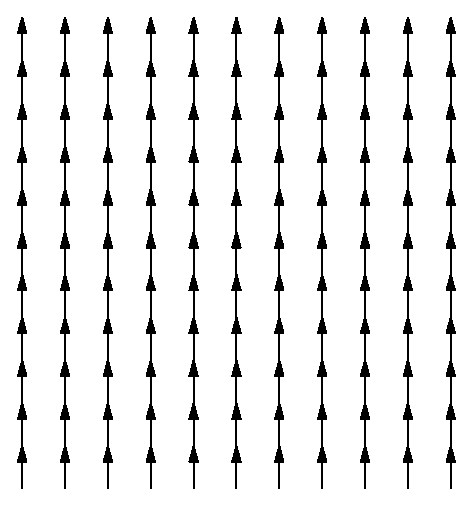
\includegraphics[width=8cm]{figure06.eps}
\caption{The Vector Field $F(x,y) = (0,1)$}
\label{figure-vector-field1}
\end{figure} 

\begin{example}
Consider the constant vector field $F(x,y) = (0,1)$ on
$\RR^3$, as seen in figure \ref{figure-vector-field1}. The
vector $(0,1)$ is a unit vector in the vertical y-axis
direction in $\RR^2$. This vector fields associates that unit
vertical vector to each point in $\RR^2$ (in local
coordinates). At each point, the vector points vertically
upward from that point. If this field represented a fluid
flow, the fluid would be flowing upwards (in $y$) at a
uniform pace everywhere, following these local direction
vectors. 
\end{example}

\begin{defn}
If $F: \RR^n \rightarrow \RR^n$ is a vector field, then we can
write $F = (F_1, F_2, \ldots, F_n)$ in terms of its
\emph{components}. Each component $F_i$ is itself a scalar
field, has partial derivatives and gradients, and is
subject to all the tools we already have for scalar fields. 
\end{defn}

We can also use all the tools of vector analysis to understand
vector fields. If $F: \RR^n \rightarrow \RR^n$ is a vector
field, then $|F|$ is the length of each vector.
$\frac{F}{|F|}$ is the unit vector in each direction of $F$ as
long as $|F|$ is not zero. If $G$ is another vector field, then
we can calculate the scalar field $F \cdot G$ at each point. If
$n=3$, we can also calculate $F \times G$. If $f: \RR^n
\rightarrow \RR$ is a scalar field, then the multiplication
$fF$ is a scalar multiplication of the vector $F$ on each
point in the domain of both functions. $F + G$ and $F-G$ are
also vector fields, formed by adding or subtracting vectors.
The expression $FG$ doesn't make any sense, since we can't
multiply vectors. 

\begin{figure}[t]
\centering
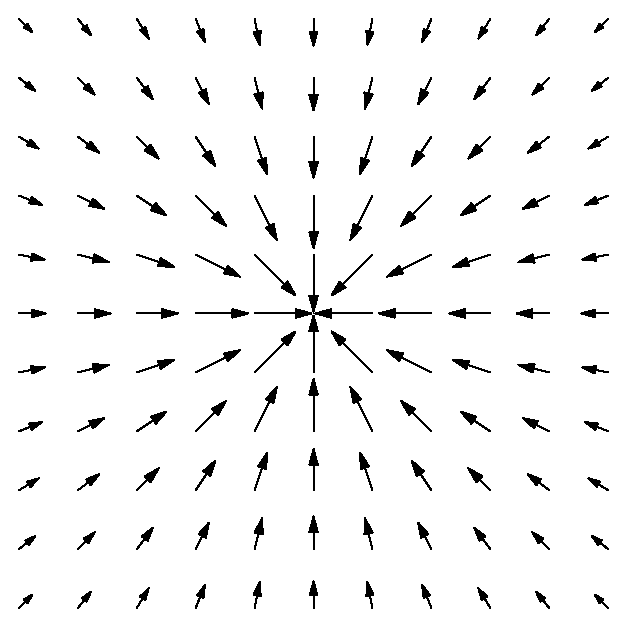
\includegraphics[width=8cm]{figure07.eps}
\caption{The Vector Field Describing Gravitational Force}
\label{figure-vector-field2}
\end{figure} 

\begin{example}
An excellent example of a vectors field is the 
force of gravity, shown in Figure \ref{figure-vector-field2}.
The magnitude of the force of gravity per unit mass due to a
mass $M$ at the origin is a scalar field.
$(x,y,z)$ is:
\begin{equation*}
f = \frac{MG}{x^2+y^2+z^2}
\end{equation*}
However, the force itself also includes direction, so it is a
vector field.
\begin{equation*}
F = \frac{MG}{(x^2+y^2+z^2)^{\frac{3}{2}}} (-x,-y,-z)
\end{equation*}
The direction $(-x,-y,-z)$ is back towards the origin. 
We can recover the magnitude by taking the length of the
vector.
\begin{equation*}
|F| = \frac{MG}{(x^2 + y^2 + z^2)^\frac{3}{2}} \sqrt{x^2
+y^2+z^2} = \frac{MG}{x^2 +y^2+z^2} = \frac{MG}{r^2}
\end{equation*}
\end{example}

\section{Integral Curves}
\label{integral-curves}

\begin{figure}[t]
\centering
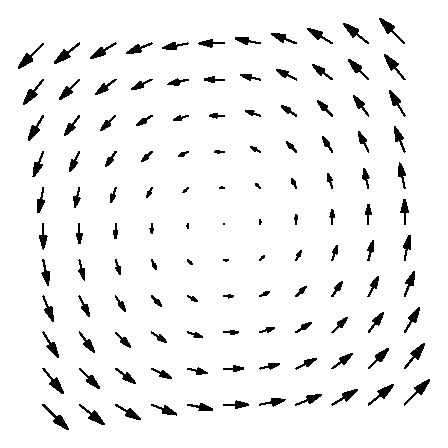
\includegraphics[width=6cm]{figure02.eps}
\caption{The Vector Field $F(x,y) = (-y,x)$}
\label{figure-vector-field3}
\end{figure}

\begin{figure}[t]
\centering
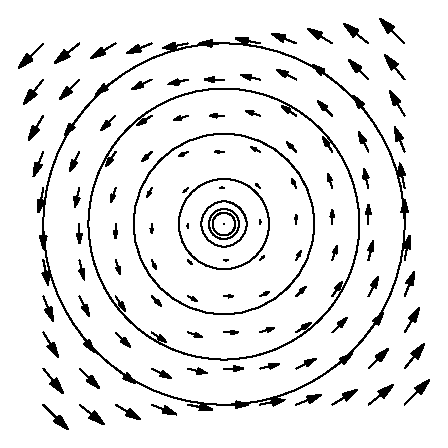
\includegraphics[width=6cm]{figure03.eps}
\caption{The Integral Curves for $F(x,y) = (-y,x)$}
\label{figure-vector-field3-curves}
\end{figure}

If we interpret a vector field as a fluid flow, imagine a
bouyant object floating in the flow. Moving with the flow,
what path would the bouyant object take? More mathematically, 
given the arrows of direction of a vector field, can we find parametric
curves $\gamma(t)$ which follow these arrows? What does
follow mean? 

\begin{defn}
Let $F: S \rightarrow \RR^m$ be a vector field on a region $S
\subset \RR^n$. If there exists a family (depending on some
variable $a \in \RR^k$) of parametric curves $\gamma_a$ such
that, over the whole family, $\gamma^\prime(t) = F$, then
these parametric curves are called the \emph{integral curves}
of the vector field. That is, the \emph{tangents} of the
parametric curves are the same as the vector field everywhere.
Equivalently, a parametric curve $\gamma(t)$ is an integral
curve for a vector field $F$ if $\gamma^\prime(t) =
F(\gamma(t))$. 
\end{defn}

\begin{example}
Consider the vector field $F(x,y) = (-y,x)$, as shown in
Figure \ref{figure-vector-field3}, with its integral curves.
These integral curves of $F(x,y) = (-y,x)$ aren't surprising.
Looking just at the vector fields, we can clearly
tell that the fluid is travelling in a circular paths.
Mathematically, the circles are curves $\gamma(t) = (a \cos t,
a \sin t)$ for a parameter $a > 0$. We can calculate
$\gamma^\prime(t) = (-a\sin t, a \cos t) = (-y, x)$. In terms
of the curve coordinates, these tangents are exactly the
vector field.
\end{example}

\begin{figure}[t]
\centering
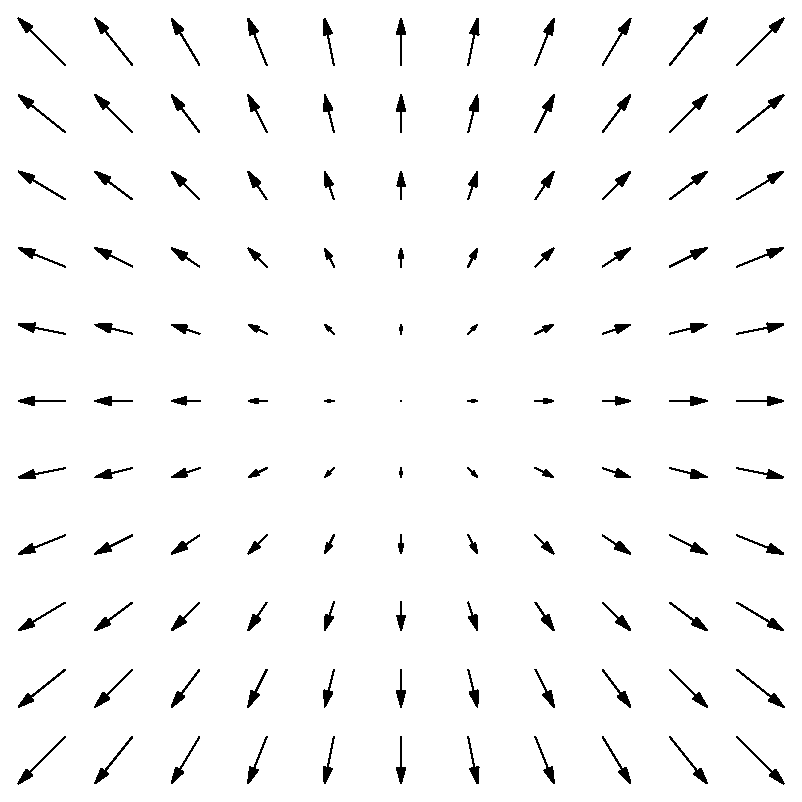
\includegraphics[width=6cm]{figure04.eps}
\caption{The Vector Field $F(x,y) = (x,y)$}
\label{figure-vector-field4}
\end{figure}

\begin{figure}[t]
\centering
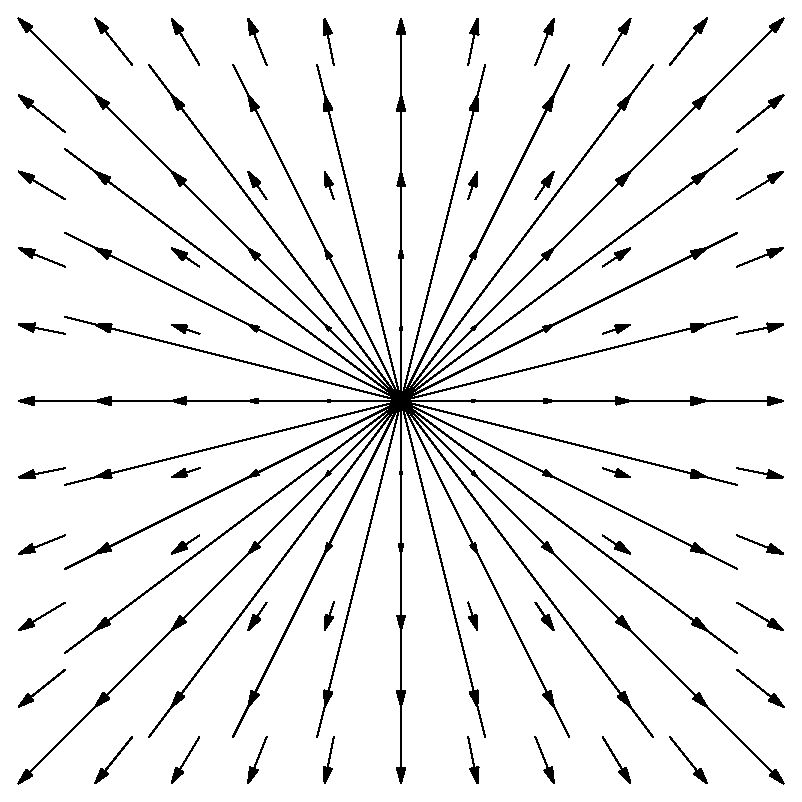
\includegraphics[width=6cm]{figure05.eps}
\caption{Integral Curves for $F(x,y) = (x,y)$}
\label{figure-vector-field4-curves}
\end{figure}

\begin{example}
Let $F(x,y) = (x,y)$, as in Figure \ref{figure-vector-field4}.
The curves $\gamma(t) = (ae^t,be^t)$ where $a,b \in \RR$ are
integral curves. They have $x = ae^t$ and $y = be^t$, and we
can calculate tangents: $\gamma^\prime(t) = (ae^t, be^t) =
(x,y)$. 
\end{example}

Integral curves are a very powerful conceptual tool. However,
they are usually very hard to calculate and most examples are
beyond the scope of this course. However, there will be a few
we can attempt. I'll describe the general process in $\RR^3$.

If $F = (F_1,F_2,F_3)$ is a vector field and $\gamma(t) =
(\gamma_1, \gamma_2,\gamma_3)$ is a parametric curve, then
$\gamma$ is an integral curve if it satisfies the following
system.
\begin{align*}
\gamma_1^\prime(t) & = F_1(\gamma_1, \gamma_2, \gamma_3) \\
\gamma_2^\prime(t) & = F_2(\gamma_1, \gamma_2, \gamma_3) \\
\gamma_3^\prime(t) & = F_3(\gamma_1, \gamma_2, \gamma_3)
\end{align*}
This is a system (generally non-linear) of three
differential equations in three functions, the $\gamma_i$.
Even if it is linear, this is still a difficult system to
solve, if not impossible. Even a simple
field such as $F(x,y,z) = (y,z,x)$ leads to a difficult
system.
\begin{align*}
\gamma_1^\prime & = \gamma_2 \\
\gamma_2^\prime & = \gamma_3 \\
\gamma_3^\prime & = \gamma_1 
\end{align*}
Currently, we have no method for approaching this system. The
solution would be a function which is its own third
derivative, and we are not currently aware of any such
functions. However, there are some approach examples with
reasonable systems of equations.

\begin{example}
Let $F = (x,y,z)$.
\begin{align*}
\gamma_1^\prime & = \gamma_1 \implies \gamma_1(t) = ae^t \\
\gamma_2^\prime & = \gamma_2 \implies \gamma_2(t) = be^t \\
\gamma_3^\prime & = \gamma_3 \implies \gamma_3(t) = ce^t \\
\end{align*}
\end{example}

\begin{example}
Let $F = (1,2x,3y)$. 
\begin{align*}
\gamma_1^\prime & = 1 \\
\gamma_2^\prime & = 2\gamma_1 \\
\gamma_3^\prime & = 3\gamma_2 
\end{align*}
This can be solved iteratively.
\begin{align*}
\gamma_1 & = \int 1 dt = t + a \\
\gamma_2 & = 2\int \gamma_1 dt = \int 2t + 2a dt = t^2 + 2at + b
\\
\gamma_3 & = 3 \int \gamma_2 dt = \int 3t^2 + 6at + 3b dt = t^3
+ 3at^2 + 3bt + c \\
\gamma(t) & = (t+a, t^2 + 2ta + b, t^3 + 3at^2 + 3bt + c) 
\end{align*}
\end{example}

\section{Vector Operations on Vector Fields}
\label{vector-operations}

Recall the gradient $\nabla f$ of a scalar field $f$. It's
useful to recall the definition of the operator $\nabla$. 
(stated in $\RR^3$ for convenience).
\begin{equation*}
\nabla = \left( \frac{\del}{\del x}, \frac{\del}{\del y},
\frac{\del}{\del z} \right)
\end{equation*}
If $f$ is a scalar field, then the gradient $\nabla f$ is a
\emph{vector field} describing the direction of greatest
change. We didn't investigate it's propreties as a vector
field in Calculus III, but it was the first vector field we
used.

There are new operators we can define using $\nabla$
on vector fields $F$. $\nabla$ operates a vector,
since is has components which are differential
operators. Therefore, we use vector notation involving
$\nabla$.

\begin{defn}
Let $F : \RR^3 \rightarrow \RR^3$ be a vector field. The
\emph{curl} of $F$ is defined as the
the cross product of $\nabla$ and $F$. Note that this outputs
a new vector field, not a scalar field.
\begin{equation*}
\nabla \times F = \left( 
\frac{\del F_3}{\del y} - \frac{\del F_2}{\del z}, 
\frac{\del F_1}{\del z} - \frac{\del F_3}{\del x}, 
\frac{\del F_2}{\del x} - \frac{\del F_1}{\del y}, 
\right) 
\end{equation*}
\end{defn}

Curl measures the tendency of the vector field
to cause \emph{local} rotation. If we think of the
vector field as a fluid flow and if we drop an object in the
fluid, it will flow along the integral curves of the vector
field. However, as it flows along, it may also start spinning
about its own axis. Curl measure the tendency of the vector
field to cause such a spin. (This is very different from
global rotation. The paths of rotation themselves may be
circular without actually causing the object itself to spin.
Likewise, the paths can be totally straight but still cause
rotation.) 

\begin{defn}
A vector field with zero curl is called \emph{irrotational}.
\end{defn}

\begin{example}
Consider $F(x,y,z) = (y,0,0)$. This is a field
which moves objects in the $x$ direction, but the speed of
movement varies with the $y$ coordinate. The curl is $\nabla
\times F = (0,0,-1)$. This field causes a clockwise rotation
about the $z$ axis; as particles in the fluid move in the $x$
direction, they start spinning around a vertical axis. 
\end{example}

\begin{defn}
Let $F: \RR^n \rightarrow \RR^n$ be a vector field in any
dimension. The \emph{divergence} of $F$ is the dot product $\nabla \cdot
F$. Note that this outputs a new scalar field, not a vector
field.
\begin{equation*}
\nabla \cdot F = \frac{\del F_1}{\del x_1} + \frac{\del
F_2}{\del x_2} + \ldots + \frac{\del F_n}{\del x_n}
\end{equation*}
\end{defn}

The divergence measure the tendency of a vector field to
diffuse. Thinking in terms of gaseous fluids, a positive
divergence at a point means that the density of the gas is
\emph{decreasing}. Some directions of flow may be inward and
some outward, but there is a net diffusion of the gas. If the
divergence is negative, the density is \emph{increasing} and there
is a net gathering of the gas. 

\begin{defn}
A vector where where the divergence is zero
is called \emph{incompressible}.
\end{defn}

Many liquids are incompressible, at least locally and under
reasonable energy circumstances. Water is usually treated as
an incompressible fluid. The major difference in fluid
dynamics between gases and liquid is compressibility.

\begin{defn}
Let $f$ be is a scalar field $\RR^n \rightarrow \RR$. It's
\emph{Laplacian} is the divergence of its gradient: $\nabla
\cdot (\nabla f) = \nabla^2 f$. Note that this outputs a
scalar field.
\end{defn}

The Laplacian was mentioned in the previous
term, since the input and output are both scalar fields.
However, the intermediate state (the gradient) is a vector
field, and the second part of the operation (the divergence)
is a vector operation. This persepctive of the Laplacian is
quite useful. 

The Laplacian is very important for many differential
equations in physics. As the divergence of the gradient
field, it measures where the scalar field leads to a gathering
or spreading. In a potential energy field, it measures the
sources (attractors) and repellors which generate the field.

There were two important differential equations introduced in 
Calculus III: the heat equation and the wave equation.
Extending these DES to several dimensions uses the Laplacian.
Recall the 1-variable and multi-variable versions of those
two equations.
\begin{align*}
\frac{\del f}{\del t} & = \alpha \frac{\del^2 f}{\del x^2} \\
\frac{\del^2 f}{\del t^2} & = \alpha \frac{\del^2 f}{\del x^2} 
\end{align*}
Replacing the 1-variable position derivative with a
multivariable Laplacian extends these DEs to several
variables.
\begin{align*}
\frac{\del f}{\del t} & = \alpha \nabla^2 f \\
\frac{\del^2 f}{\del t^2} & = \alpha \nabla^2 f \\
\end{align*}
We've also seen the Laplacian in the Schr\"odinger
equation and the Navier-Stokes equation as the space
derivative term. 

In the wave equation, if $\nabla^2 f = 0$ then $\frac{\del^2
f}{\del t^2} = 0$. Therefore, $f$ has, at most, a linear
dependence in $t$. Since the dependence in $x$ is often
sinusoidal, a common solution here is a standing wave or a
wave with constant velocity. This (among other, more
confusing reasons) leads to the terminology of harmonic
functions. 

\begin{defn}
A scalar field $f$ is \emph{harmonic} if $\nabla^2 f = 0$
\end{defn}

The harmonic condition is a very 
restrictive condition. In particular, harmonic functions
satify a maximum modulus
principle: if $f$ has an strict extrema in an open set, then
it has a point with non-zero Laplacian and cannot be harmonic.
Therefore, the extrema of $f$ must always come on the boundary
of any open set. In complex analysis, all differentiable
(holomorphic) functions are harmonic; this fact leads to very
different behaviour between real and complex differentiable
functions.

\subsection{Interaction between Vector Operations}
\label{interactions}

All uses of $\nabla$ are linear.

\begin{prop}
Let $f$ and $g$ be scalar fields on $\RR^3$, and let $F$ and
$G$ be vector fields on $\RR^3$. Let $a$ and $b$ be
constants. Then:
\begin{align*}
\nabla (af \pm bg) & = a \nabla f \pm b \nabla g \\
\nabla \times (aF \pm bG) & = a (\nabla \times F) \pm b (\nabla
\times G) \\
\nabla \cdot (aF \pm bG) & = a (\nabla \cdot F) \pm b (\nabla
\cdot G) \\
\nabla^2 (af \pm bg) & = a \nabla^2 f \pm b \nabla^2 g \\
\end{align*}
\end{prop}

In the previous identity (and similar identities), pay careful
attention to which outputs are scalar fields and which are
vector fields.

Since $\nabla$ is a differential operator, it doesn't
distribute over multiplication. However, there are
several generalizations of the Leibniz rule.

\begin{prop}
Let $f$ be a scalar field on $\RR^3$ and let $F$ and $G$ be
vector fields on $\RR^3$. 
\begin{align*}
\nabla \cdot (F \times G) & = (\nabla \times F) \cdot G - F
\cdot (\nabla \times G) \\
\nabla \cdot (fF) & = f (\nabla \cdot F) + (\nabla f) \cdot F
\\
\nabla \times (fF) & = f (\nabla \times F) + (\nabla f) \times
F
\end{align*}
\end{prop}

In the first Leibniz rule we have a difference instead of the
expected sum. In general versions of the Leibniz rule, this
negative sign is quite common. Many versions of the rule have
$(-1)^k$ for some $k$, showing that it is equally easy to have
a sum or difference.

There are two important results about composition of vector
operations.

\begin{prop}
Let $f$ be a scalar field on $\RR^3$ and $F$ a vector field on
$\RR^3$. Then $\nabla \times (\nabla f) = 0$: the 
curl of a gradient is zero. Also, $\nabla \cdot (\nabla
\times F) = 0$: the divergence of a curl is zero.
\end{prop}

This proposition is established by calculating all the
terms and using the compatibility of order in mixed second
partial derivatives. The proofs are left as exercises. 

This proposition is also a 
glimpse of a very general result in analysis. If we work with
the right definitions, applying the same (or similar)
differential operator twice in a row should give the zero
operator. Obviously, this isn't always true:
partial derivatives certainly don't satisfy this, and even for
$\nabla$, $\nabla \cdot \nabla f \neq 0$ for a
general scalar field. Near the end of these notes, we will
give a general structure for understanding why differential
operators should compose to zero. 

\begin{example}
Consider the scalar field $f(x,y) = \ln (x^2 + y^2)$, which is
defined everywhere except the origin. 
\begin{align*}
\nabla f & = \left( \frac{2x}{x^2 + y^2}, \frac{2y}{x^2+y^2}
\right) \\
\nabla^2 f & = \frac{2}{x^2 + y^2} - \frac{4x^2}{(x^2 + y^2)^2} +
\frac{2}{x^2+y^2} - \frac{4x^2}{(x^2+y^2)^2} = 0 
\end{align*}
This is a harmonic scalar field. In particular, it can have
no extrema on an open set. Values approach $-\infty$ near the
origin and $\infty$ as we get very far from the origin.
\end{example}

\begin{example}
Consider the vector field $F(x,y,z) = (-z,x,-y)$. $\nabla
\times F = (-1,1,1)$, so the vector field causes the same
local rotation at all points, about the axis $(-1,1,1)$ (as a
local axis direction). $\nabla \cdot F = (0,0,0)$, so the
flow is incompressible. This is a good field to potentially
model a liquid flow that induces a particular local rotation
everywhere.
\end{example}

\begin{example}
Consider the vector field $F(x,y,z) = (x^2,y^2,z^2)$. $\nabla
\times F = (0,0,0)$, so the field is irrotational. The
divergence is $\nabla \cdot F = (2x +2y+2z)$. In the positive
octant, the flow accelerates away from the origin, so the rate
of difussion increases away from the origin In other octants,
we may have negative divergence, reflecting the fact that the
local vector field directions are always positive.
\end{example}

\begin{example}
Consider the vector field $F(x,y,z) = (-y,x,0)$ (which should
be fairly familiar by this time). $\nabla \times F =
(0,0,2)$, which shows the creation of local rotation about the $z$
axis. Note that this is local rotation, which is seperate
from the global rotation of the integral curves about the
origin. Also, $\nabla \cdot F = 0$, so the flow is
incompressible. As the flow spins around, it neither collects
or diffuses anywhere.
\end{example}

\begin{example}
Consider the vector field $F(x,y,z) = (\sin x, \cos y, 0)$.
$\nabla \times F = (0,0,0)$, so the flow is irrotational.
This is interesting, given the trigonometric term;
trigonometry might cause us to expect spin. $\nabla \cdot F = \cos
x - \sin y$, so there are various areas of diffusion and
collection. The trigonometric term here causes
diffusion/collection, not rotation.
\end{example}

\begin{example}
Consider the vector field $F(x,y,z) = \left( \frac{1}{x+y},
\frac{1}{x+y}, 0 \right)$. $\nabla \times F = \left(0,0,
\frac{-1}{(x-y)^2} - \frac{-1}{(x+y)^2} \right)$: this curl is
always negative and always about the $z$ axis. $\nabla \cdot F
= \frac{-1}{(x+y)^2} + \frac{1}{(x-y)^2}$: therefore,
$F$ collects when $x$ and $y$ are dissimilar and diffuses
when $x$ and $y$ are quite close. 
\end{example}

\section{Conservative Vector Fields}
\label{conservative}

An important class of vector fields are gradients of scalar
fields. The most common case is a potential energy scalar
field, where $f$ measures potential energy. A principle of
motion in physics states that particles will seek to lower
their potential energy in the most efficient way possible.
That is, they will move in the direction of greatest descent
of potential energy. That movement is precisely along the
integral curves of the vector field $\nabla f$. So, if we try
to explain a physical situation by a potential energy field,
then the movement of particles is equivalent to finding
integral curves of $\nabla f$. Moreover, movement along these
paths creates kinetic energy. The speed of movement can be
determined by conservation of energy: the movement along the
paths has speed and kinetic energy gained at exactly the same
rate as potential energy is lost. Conservation of energy
explains the terminology of this section. 

\begin{defn}
Let $f$ be a scalar field. Then field $\nabla f$
created from a potential energy field is called a
\emph{conservative vector field}.
\end{defn}

If we are given a general vector field $F$, we would like to
check whether or not it is conservative. We have the identity
$\nabla \times \nabla f=0$, which shows that all conservative
fields are irrotational. Is the converse true? We need a
technical definition before we can answer this question.

\begin{defn}
Let $U$ be an open subset of $\RR^n$. $U$ is called
\emph{path connected} if there is a parametric curve
connecting any two points $a, b \in U$. (Recall in our
definition in Calculus III that parametric curves are always
continuous.) If $U$ is path
connected, it is also called \emph{simply connected} if any
closed path (a path which starts and ends at the same spot) can
be contracted down to a point. (Think of the path as a loop
in a rope, and contraction as pulling the rope so that the
loop disappears. This needs to happen in such a way that all
the intermediate steps are still paths in the set $U$). 
\end{defn}

Na\"ively, a simply connected set has no holes in it. A
solid cylinder is simply connected. However, the hollow
cylinder is not, since a loop around the cylinder can never be
contracted.

\begin{prop}
Let $U$ be a simply connected open set in $\RR^3$ and let $F:
U \rightarrow \RR^3$ be a differentiable vector field 
Then $F$ is conservative on $U$ if an only if $\nabla \times F = 0$.
\end{prop}

The condition $\nabla \times F$ works both ways under a
reasonable condition for the domain of the vector field. We
can check if a vector is conservative by taking the curl; if
the curl is zero, it is conservative.

If $F$ is conservative, then there exists at least one (in
fact, infinitely many!) scalar fields $f$ with $F = \nabla f$.
This $f$, inspired by the physics situation, is called a
(scalar) potential for $F$. If $f$ is a potential energy
field, $F$ is the associated field of force. Usually, both
the potential energy and force fields are defined per unit
mass or charge, so that they can act on any mass or charge
present in the field.


How do we calculate $f$? The equation $F = \nabla f$ can be
expanded. 
\begin{align*}
F_1 & = \frac{\del f}{\del x} \\
F_2 & = \frac{\del f}{\del y} \\
F_3 & = \frac{\del f}{\del z} 
\end{align*}
We can integrate each of these equations. We have to be
careful with the `constants': in each integral, the constants
can be functions of both of the remaining variables. 
\begin{align*}
f & = \int F_1 dx + g_1(y,z) \\
& = \int F_2 dy + g_2(x,z) \\
& = \int F_3 dz + g_3(x,y) 
\end{align*}
Finding $f$ amounts to finding a scalar field that fits this
system. For reasonable $F$, this isn't too terrible. We
expect a family of solutions: since we are integrating and
there will be constants of integration introduced. Initial
values can determine the constant to give a unique potential.
The constants here make sense: potential energy is always a
relative measure, so we have to set a base level of potential
energy. Please note: energy is always relative! Unlike mass
and charge, energy is not an intrinsic measure. Energy is a
fiction, but a very useful fiction for explaning motion.

\section{Line Integrals of Vector Fields}
\label{line-integrals}

As the start of this course, We integrated scalar fields over
various regions in $\RR^3$. Now that we have defined vector
fields, we can ask if there is a reasonable definition for
integration of a vector field. This seems like an odd
question: integrating scalar fields, such a density, made
sense. What does it mean to integrate a vector field?

We will start with integrating along a parametric curve.
If we think of the vector field as a force field, then the integral of
the vector field along the path will be interpreted as the
\emph{work} to move through the field. Alternatively, we can
interpret the line integral as the work that the field
accomplished to move the object. (The sign of the vector field
can be changed to accomodate this variable perspective:
working with or working against the field.)

If $F$ represents resistance to movement, like walking into
the wind, then we look at the vectors as directions pushing
with or against the movement. If $\gamma$ is movement through a
vector field, then its local direction at any moment is its
tangent $\gamma^\prime(t)$. To determine whether or not we
are moving into the wind, with the wind, or sideway through
it, we have to compare the vector field and the tangent.
We use dot product: $F \cdot \gamma^\prime(t)$ is large if the
vectors share a direction and zero when the vectors are
perpendicular.

However, we want this integral to only depend on the path, not
the parametrization. Therefore, we should use attributes of
the curve which are not dependant on the parametrization. The
unit tangent $T(s)$ is one such attribute (in terms of the
arclength parameter $s$. $F \cdot T$
measures the interaction of the movement along the curve with
the vector field. The arclength infinitesimal $ds$ is
independent of parametrization. We use these tools to give the
definition.

\begin{defn} 
The \emph{line integral} of a vector field $F$ along a path
$\gamma(s): [0,L] \rightarrow \RR^n$ is the integral of the
scalar $F(\gamma(s)) \cdot T(s)$ along the length of the
curve.
\begin{equation*}
\int_{\gamma} F \cdot T ds = \int_{\gamma} F \cdot ds \defeq
\int_0^L F(\gamma(s)) \cdot T(s) ds 
\end{equation*}
The first notation is more complete, but the shorter second
notation is conventional. 
\end{defn} 

Using the arclength parameter for the definition if
appropriate but inconvenient for calculation. 
Let $\gamma(t)$ be an arbitrary parametrization. Then we can
think of $s(t)$ (the arclenth of the curve in terms of $t$) as
a substitution of single variable integration. This
substitution has $ds = |\gamma^\prime(t)| dt$ and $T =
\gamma^\prime(t) / |\gamma^\prime(t)|$, and the new bounds are
$0$ and $L$, the length of the curve. We can then transform
the integral in the definition.
\begin{equation*}
\int_{\gamma} F \cdot T ds = \int_0^L F(\gamma(s)) \cdot T(s)
ds = \int_a^b F(\gamma(t)) \cdot
\frac{\gamma^\prime(t)}{|\gamma^\prime(t)|} |\gamma^\prime(t)|
dt = \int_a^b F(\gamma(t)) \cdot \gamma^\prime(t) dt 
\end{equation*}

The line integral measures the work or effort it takes to move
along the path through the vector field. It integral doesn't
depend at all on the speed of moving through the vector field,
since it is independent of the parametrization. The line
integral is positive if it generally goes with the direction
of the field and negative if it generally goes against. Since
moving with $F$ is positive and moving against $F$ is
negative, we sometime will want to replace $F$ with $-F$ when
we want to think of working against the field as positive work.

\begin{example}
Let's do a classic example: the force of gravity. We've
already discussed the field (per unit mass) generated by a
mass $M$ at the origin.
\begin{equation*}
F = \frac{GM}{\sqrt{(x^2+y^2+z^2)^3}} (-x, -y, -z)
\end{equation*}
We're going to reverse the sign here, since we want to do
positive work when we go against gravity. 
\begin{equation*}
F = \frac{GM}{\sqrt{(x^2+y^2+z^2)^3}} (x, y, z)
\end{equation*}
 Let's take an outward path $\gamma(t) = (t,t,t)$ for $t \in
[a,b]$ and $b>a>0$. Then 
\begin{align*}
\gamma^\prime & = (1,1,1) \\
F(\gamma(t)) & = \frac{GM}{\sqrt{(3t^2)^3}} (t,t,t) \\
F(\gamma(t)) \cdot \gamma^\prime(t) & = \frac{3t GM}{3\sqrt{3}
t^3} = \frac{GM}{t^2\sqrt{3}} \\
\int_{\gamma} F \cdot ds & = \int_b^a
\frac{GM}{t^2\sqrt{3}} = \frac{GM}{\sqrt{3}} \int_a^b
\frac{1}{t^2} dx \\
& = \frac{GM}{\sqrt{3}} \left. \frac{-1}{t} \right|_a^b =
\frac{GM}{\sqrt{3}} \left( \frac{1}{a} - \frac{1}{b} \right) \\
& = \frac{GmM(b-a)}{ab\sqrt{3}}
\end{align*}
If the distances $a$ and $b$ are large, but $a$ and $b$ are
close to each other, then the change $a-b$ is much more
significant than the change in the term $ab$ in the
denominator. If we call $g = \frac{GM}{\sqrt{3}ab}$ and
pretend this is locally constant, the line integral
(approximately) evaluates to $g(b-a)$. Recall we were working
with force per unit mass, so if we act on a mass $m$ we get a
change in potential of $mg(b-a)$. This is the familiar
high-school physics result of $mgh$, the increase in potential
energy, here $h$ is the change in height and $g$ the local
acceleration due to gravity. (Proving that our expression for
$g$ is the local acceleration due to gravity is a little
tricky, but we can see, using the fact that $G$ has units
$m^3/(kg \cdot s^2)$, that the units of $g$ are $m/s^2$, so it
is an acceleration term).
\end{example}

\begin{example}
For another example, consider the rotational flow $F(x,y) =
(-y,x)$ and $\gamma(t)$ the counterclockwise circle $(r \cos
t, r \sin t)$ for $t \in [0, 2\pi]$. 
\begin{align*}
\gamma^\prime(t) & = (-r \sin t, r \cos t) \\
F(\gamma(t)) & = (-r\sin t, r \cos t) \\
F(\gamma(t)) \cdot \gamma^\prime(t) & = r^2 \sin^2 t + r^2
\cos^2 r = r^2 \\
\int_{\gamma} F \cdot ds & = \int_0^{2\pi} r^2 dr = 2\pi r^2
\end{align*}
The work to more around the circle (with the vector field) of
radius $r$ is $2\pi r^2$. Since it is positive and follows
the integral curve, we can think of it as the work the
field accomplished to move the object along its integral
curve.
\end{example}

\subsection{Fundamental Theorems}
\label{fundamental-theorems}

Let's return to a version of the Fundamental Theorm of Calculus. 
Let $f(x)$ be a differentiable function.
\begin{equation*}
\int_a^b \frac{df}{dx} dx = f(b) - f(a)
\end{equation*}
This integration takes place on the interval $[a,b]$ and is
evaluated at the end points $a$ and $b$. We can think of the
endpoints as the \emph{boundary} of the interval. With this
perspective, the left side is the integral of some kind of
derivative and the right side is the evaluation of the
original function on a boundary. If we let $df$ be any kind of
derivative, and $\int_{\del S}$ be an integral which relates
to the boundary of a set, then when can write the archtypical
form of this theorem.
\begin{equation*}
\int_S df = \int_{\del S} f
\end{equation*}
For the fundamental theorem, the `integral' on the right-hand
side is just evaluation, since the boundary is only the two
points. Integration over a zero-dimensional regions, such as
a set of points, is just evaluation. Using this integration
notation, the fundamental theorem is only the first of a whole
family of theorems of this type. They all relate a derivative
operator on the left to a boundary operator on the right. 

\subsection{The Fundamental Theorem of Line Integrals}
\label{fundamental-theorem-line-integrals}

The first of these new fundamental theorems comes from
thinking about line integrals of paths through conservative
vector fields. 

\begin{thm}
Let $F = \nabla f$ be a conservative vector field with
potential $f$ and let $\gamma(t): [a,b] \rightarrow \RR^n$ be
a parametric curve. The fundamental theorem of line integrals
shows we can solve this integral by evaluation on the
endpoints of the curve.
\begin{equation*}
\int_{\gamma} F \cdot ds = f(\gamma(b)) - f(\gamma(a))
\end{equation*}
\end{thm}

\begin{proof}
We calculate the integral in steps. 
\begin{align*}
\int_{\gamma} F \cdot ds & = \int_{\gamma} \nabla f \cdot T
ds \\
& \int_a^b \nabla f(\gamma(t)) \cdot \gamma^\prime(t) dt \\
& = \int_a^b \left( \frac{\del f}{\del x} (\gamma(t)),
\frac{\del f}{\del y} (\gamma(t)), \frac{\del f}{\del z}
(\gamma(t)) \right) \cdot \left( \gamma_1^\prime(t),
\gamma_2^\prime(t), \gamma_3^\prime(t) \right) dt \\
& = \int_a^b \frac{\del f}{\del x} (\gamma(t))
\gamma_1^\prime(t) + \frac{\del f}{\del y} (\gamma(t))
\gamma_2^\prime(t) + \frac{\del f}{\del z} (\gamma(t))
\gamma_3^\prime(t) dx \\
& = \int_a^b \frac{d}{dt} \left( f(\gamma(t)) \right) dt \\
& = f(\gamma(b)) - f(\gamma(a))
\end{align*}
We used multi-variable chain rule in the fourth
line of the calculation. 
\end{proof}

Side by side, we can see the similarity of the theorem with
the original fundamental theorem: derivatives on one side and
(evaluation on) boundaries on the other side.
\begin{align*}
\int_a^b \frac{df}{dx} dx & = f(b) - f(a) \\
\int_{\gamma} \nabla f \cdot ds & = f(\gamma(b)) -
f(\gamma(a))
\end{align*}

\subsection{Implications for Conservative Vector Fields}
\label{implications-conservative}

The fundamental theorem for line integral applies to
conservative vector fields: it says that the integral of a
conservative vector field can be calculated simply by
evaluation on the end points. That means all the points on
the path inbetween are irrelevant!

\begin{prop}
Let $F = \nabla f$ be a conservative vector field. Then line
integrals of $F$ are \emph{path-independent}. Their value
only depends on the endpoints.
\end{prop}

No matter how strange the path is, no matter how
many times it loops around and goes elsewhere, only the
endpoints matter. If
$f$ is potential energy, then $f(\gamma(b)) - f(\gamma(a))$ is
the potential energy at the end less the potential energy
at the start. This difference is the change in potential energy.
The work to move through the force field is equal to the
change in potential energy. The work can be defined in terms
of kinetic energy lost or gained, so this says that the kinetic
energy lost or gained is equal to the change in potential
energy. Therefore, energy is conserved! This explains the
term `conservative vector field': these are vector fields
where conservation of energy makes sense. (As before, there are
sign issues in the fiction of energy and work: we may need to
take the negative of the usual or expected potential energy to
make conservation of energy make sense.)

We can calculate very explicitly in terms of the gain in
kinetic energy as well. Let $F = \nabla f$ be a conservative
force. Then $F = ma$, where $a$ is acceration. Also, if
$\gamma$ is a curve representing movement, then
$\gamma^{\prime \prime}$ is the acceleration. Then we look
carefully at the change in potential energy using our new
theorem.
\begin{align*}
-\Delta PE & = f(\gamma(b)) - f(\gamma(a)) \\
& = \int_{\gamma} F \cdot T ds \\
& = \int_a^b m \gamma^{\prime \prime}(t) \cdot
\gamma^\prime(t) dt \\
& = \frac{m}{2} \int_a^b \frac{d}{dt} (\gamma^\prime(t) \cdot
\gamma^\prime(t)) dt \\
& = \frac{m}{2} \int_a^b \frac{d}{dt} |\gamma^\prime(t)|^2 dt
\\
& = \frac{m}{2} |\gamma^\prime(t)|^2 \bigg|_a^b \\
& = \frac{mv_b^2}{2} - \frac{mv_a^2}{2} = \Delta KE
\end{align*}

Previously, we saw that conservative vector fields we
irrotational and, conversely, an irrotation field
\emph{defined on a simply connected set} was guaranteed to be
conservative. We now have a new characterization of
conversative fields: their line integrals are path
independent. We can similarly ask if the converse holds and
again, we find a topological condition. First, we start with a
slightly more narrow proposition.
\begin{prop}
Let $F$ be a vector field on $U$ an open path-connected set in
$\RR^n$. If $\int_{\gamma} F = 0$ for \emph{all} closed
paths $\gamma$ in $U$, then $F$ is conservative. 
\end{prop}

A full characterization of conservative fields is given by
this more-complete proposition.

\begin{prop}
Let $F$ be a vector field on $U$ an open simply-connected set
in $\RR^n$ and let $\gamma: [a,b] \rightarrow U$ be a
parametric curve. The following four conditions are
equivalent.
\begin{smallparts}
\item $F$ is conservative on $U$. (By
definition, this means $F = \nabla f$ for a scalar field $f$).
\item The line integrals of $F$ are path independent in $U$.
\item The line integral of $F$ is zero for any closed path in
$U$.
\item $\nabla \times F = 0$.
\end{smallparts}
\end{prop}

\subsection{Examples of Conservative Vector Fields}
\label{conservative-examples}

\begin{example}
If $F = (y \cos (xy), x \cos (xy), 2z)$ then $F$ is defined on
$\RR^3$, which is simply connected.
\begin{align*}
\nabla \times F & = \left( \frac{\del}{\del y} 2z -
\frac{\del}{\del z} x \cos (xy), \frac{\del}{\del z} y \cos
(xy) - \frac{\del}{\del x} 2z, \frac{\del}{\del x} x \cos (xy)
- \frac{\del}{\del y} y \cos (xy) \right) \\
& = (0, 0, \cos xy - xy \sin xy - \cos xy + xy \sin xy) =
(0,0,0)
\end{align*}
Therefore, $F$ is a conservative field. We can try to
calculate its potential.
\begin{align*}
f & = \int y \cos (xy) dx + g_1(y,z) = \sin (xy) + g_1(x,y) \\
f & = \int x \cos (xy) dy + g_2(x,z) = \sin (xy) + g_2(x,z) \\
f & = \int 2z dz + g_3(x,y) = z^2 + g_3(x,y) \\
f & = \sin xy + z^2 + c
\end{align*}
We can check $\nabla f$ to see that we recover the original
field $F$. 
\end{example}

\begin{example}
If $F = (3y^z - 8xz^2 + 3x^2 y, 6xyz + x^3 + 2yz^2, 3xy^2 -
8x^2z + 2y^2z)$, then $F$ is defined on all $\RR^3$.
\begin{equation*}
\nabla \times F = (6xy+4yz-6xy-4yz, 3y^2 -16z -3y^2 + 16z, 6yz
+ 3x^2 - 3yz - 3x^2) = (0,0,0)
\end{equation*}
Therefore, $F$ is conservative. We can try to calculate its
potential.
\begin{align*}
f & = \int F_1 dx = 3xy^2 z - 4x^2 + z^2 + x^3 y + g_1(y,z) \\
f & = \int F_2 dy = 3xy^2 z + x^3 y + y^2 z^2 + g_2(x,z) \\
f & = \int F_3 dz = 3xy^2 z - 4x^2 z^2 + y^2 z^2 + g_3 (x,y)
\\
f & = 3xy^2 z - 4x^2 z^2 + x^3 y + y^2 z^2 + c
\end{align*}
\end{example}

\section{Parametric Surfaces}
\label{parametric-surfaces}

We've defined integrals of vector fields along
arametric curves. However, parametric curves are only one dimensional
objects. What does it mean to integrate a vector field over higher
dimensional objects? 

Vector fields are not like scalar fields, where we can just
integrate over regions of $\RR^3$. We take a hint from line
integrals using parametric curves: we need parametric objects.
We can define parametric objects in any dimension, though the
theory gets more and more difficult with added dimensions. In
this section we define parametric surfaces, which are the
2-dimensional analogue to parametric curves.

If $[a,b]$ is an interval on
$\RR$, a curve was a function on that interval into a vector
space.
\begin{equation*}
\gamma: [a,b] \rightarrow \RR^3
\end{equation*}
The curve is a \emph{continuous} (usually differentiable)
function on the interval. For surfaces, we need two
directions of freedom, so we start in $\RR^2$ instead of
$\RR$. We might start with intervals $I$ in $\RR^2$, but we
can be a bit more general. 

\begin{defn}
Let $D \subset \RR^2$ be a \emph{simply connected} set. A
parametric surfaces in $\RR^3$ is a \emph{continuous} (usually
differentiable) function on $D$ into a vector space.
\begin{equation*}
\sigma: D \rightarrow \RR^3
\end{equation*}
\end{defn}

Like parametric curves, we visualize surfaces only by their
outputs. The input set $D$ isn't visualized; rather, it is
thought of as the parameter space. The difference, compared to
curves, is that we now have a 2-dimensional parameter space.
This allows two independent directions of movement on the
surface.

We need to refine the previous definition a little bit: we
want to avoid places where the surface has strange behaviour
by insisting that the surface is `smooth'. Differentiability
is required here, but the condition is actually a bit
stronger. We need to think about tangents. 

For a curve $\gamma(t)$, the only derivative was the time
derivative and $\gamma^\prime(t)$ was the tangent. For a
surface, let $u$ and $v$ be the coordinates in the region $D$.
Then we have two partial derivatives: $\sigma_u =
\frac{\del}{\del u} \sigma(u,v)$ and $\sigma_v =
\frac{\del}{\del v} \sigma (u,v)$. These are both tangents. 

\begin{defn}
A parametric surface is called \emph{smooth} if it has two (linearly)
independent tangent directions at any point.
Working in $\RR^3$, we can calculate $\sigma_u \times
\sigma_v$. This is perpendicular to both tangents, so this
direction should be normal to the surface. We will
use that name, and call $\sigma_u \times \sigma_v$ the
\emph{normal} to a smooth parametric surface. 
\end{defn}

The smoothness condition can be rephrased: the normal must never
be zero. We will be using the normal extensively and
zero normals will cause many problems. Therefore, from this
point, we assume all surfaces are piece-wise smooth, with non-zero
normals. Piece-wise is enough, since the cross-over sections
will be lower-dimensions and thus can be ignored in
integration. (For curves, we made implicit use of a similar
convention that the tangent should never be the zero vector,
though we didn't say so at the time.) Since we are using the
cross-product, this definition on applies to $\RR^3$. For the
rest of this entire chapter, we will exclusive be working with
parametric surfaces in $\RR^3$.

\begin{example}
\label{example-surface-graph}
If $f(x,y)$ is a 2-variable function on a
simply-connected domain $D$, it's graph is a surface. We can
use $D$ as the domain and $\sigma (u,v) = (u,v,f(u,v))$
is the graph expressed as a parametric surface.
\end{example}

\begin{example}
\label{example-surface-revolution}
Consider a surface of rotation. If we rotate $y = f(x)$ about
the $x$ axis for $x \in [a,b]$, then we can take $\theta$ to
be other parameter and $D =[a,b] \times [0, 2\pi]$ to be the
parameter domain. Then $\sigma(x,\theta) = (x, f(x) \cos
\theta, f(x) \sin \theta)$ is the surface of revolution.
\end{example}

\begin{example}
\label{example-sphere-parametrization}
If $(\theta, \phi) \in D = [0, 2\pi] \times [0, \pi]$ then
$\sigma (\theta, \phi) = (r \sin \phi \cos \theta, r \sin \phi
\sin \theta, r \cos \phi)$ is a parametric description of the
sphere with radius $r$.
\end{example}

\begin{example}
If $(\theta, z) \in D = [0, 2\pi] \times [0,h]$ then $\sigma
(\theta, z) = (r \cos \theta, r \sin \theta, z)$ is a
parametric description of a cylinder with height $h$ and
radius $r$ oriented along the $z$-axis. 
\end{example}

\begin{example}
If $(u,v) \in D = [0,h] \times [0, 2\pi]$ then $\sigma (u,v) =
(u \cos v, u \sin v, u)$ is a parametric description of a cone
opening upwards in the $z$ direction with height $h$ and base
radius $h$ as well.
\end{example}

\section{Surface Integrals}
\label{surface-integrals}

Recall the definition of the line integral.
\begin{equation*}
\int_{\gamma} F \cdot T ds = \int_a^b F(\gamma(t)) \cdot
\gamma^\prime(t) dt 
\end{equation*}
On the left, we started with intrinsic information, using the
arclength parametrization and infinitesimal $ds$ to build a
definition which didn't depends on parametrization. Then we
showed, using $ds = |\gamma^\prime(t)| dt$ how to calculate
the line integral for an arbitrary 
the description of length in terms of the parametrization. We
have something similar for surfaces. Instead of length, we
have an infinitesimal area $dA$ which is independent of the
parametrization. If $\sigma(u,v)$ is a function of the
parameters $u$ and $v$ on a simply connected domain $D$,
through a change of variables, we can express the intrinsic
$dA$ in terms of the specific parameters $u$ and $v$. For
curves, the mediating factor was the length of the tangent;
for surfaces, it is the length of the normal.
\begin{equation*}
dA = |\sigma_u \times \sigma_v| du dv
\end{equation*}
This gives us a local area differential for integration.

\begin{defn}
Let $\sigma(u,v)$ be a parametric surface defined on a simply
connected open set $D$. Let $f$ be a scalar field defined in a
neighbourhood of the surface $\sigma$. The integral of $f$
over $\sigma$ is defined as follows.
\begin{equation*}
\int_\sigma f dA = \int_D f(\sigma(u,v)) |\sigma_u \times
\sigma_v | du dv
\end{equation*}
\end{defn}

This definition lets us calculate surface area of
parametric surfaces. To find area, we just integrate the
constant scalar field $f = 1$. 
\begin{equation*}
A = \int_\sigma 1 dA = \int_D |\sigma_u \times \sigma_v| du dv 
\end{equation*}
If we expand this out, we can get the full expression in all
its complexity.
\begin{equation*}
A = \int_D \sqrt{
\left( \frac{\del \sigma_2}{\del u} \frac{\del \sigma_3}{\del v}
- \frac{\del \sigma_2}{\del v} \frac{\del \sigma_3}{\del u}
 \right)^2 + 
\left( \frac{\del \sigma_3}{\del u} \frac{\del \sigma_1}{\del v}
- \frac{\del \sigma_3}{\del v} \frac{\del \sigma_1}{\del u}
 \right)^2 + 
\left( \frac{\del \sigma_1}{\del u} \frac{\del \sigma_2}{\del v}
- \frac{\del \sigma_1}{\del v} \frac{\del \sigma_2}{\del u} \right)^2 }
du dv
\end{equation*}

\begin{example}
Let $\sigma$ be the graph of a
function $f: \RR^2 \rightarrow \RR$ as defined in Example
\ref{example-surface-graph}. Then we can use the area formula
to write the general equation of the surface area of the graph
of $f$ over a simply-connected region $D$ in its domain.
\begin{equation*}
A = \int_D \sqrt{ \left( \frac{\del f}{\del x} \right)^2 +
\left( \frac{\del f}{\del y} \right)^2 + 1} dx dy 
\end{equation*}
\end{example}

\begin{example}
Let $f: [a,b] \rightarrow \RR$ be a differentiable function
and let $\sigma$ is a surface of
revolution as defined in Example \ref{example-surface-revolution}. Let
$D = [a,b] \times [0,2\pi]$. Then we can define the surface of such a
general surface of revolution.
\begin{equation*}
A = \int_D \sqrt{ 1 - \left( \frac{\del f}{\del x} \right)^2}
f(x) dx 
\end{equation*}
\end{example}

\begin{example}
The parabaloid $z = k(x^2 +y^2)$ can be
described by $\sigma(u,v) = (u,v,k(u^2+v^2))$ over $D$ a circle
of radius $r$. We can calculate its surface area.
\begin{align*}
A & = \int_D \sqrt{4k^2 u^2 + 4k^2 v^w + 1} du dv \\
& = \int_0^{2\pi} \int_0^r \sqrt{4k^2 r^2 + 1} r dr d \theta
\\
u & = 4k^2 r^1 + 1 \implies du = 8k^2 r dr \\
& = 2\pi \int_1^{4hk} \sqrt{u} \frac{1}{8k^2} du \\
& = \left. \frac{\pi}{4k^2} \frac{2u^{\frac{3}{2}}}{3}
\right|_1^{4kh} \\
& = \frac{\pi}{6k^2} \left( (4kh)^{\frac{3}{2}} -1 \right) =
\frac{2\sqrt{h^3k^3} - 1}{6k^2}
\end{align*}
\end{example}

\begin{example}
The surface of revolution under $f(x) = \frac{1}{x}$ for $x
\in [1,\infty)$ is called the Horn of Gabriel. It can be
described parametrically for $(x,\theta) \in [1, \infty) \times
[0, 2\pi]$ as the following surface.
\begin{equation*}
\sigma(x,\theta) = \left( x, \frac{\cos \theta}{x}, \frac{\sin
\theta}{x} \right) 
\end{equation*}
The surface area of the Horn of Gabriel is quite interesting.
(The comparison results for single-variable integrals are
useful in this calculation.) 
\begin{align*}
\sigma_x & = \left( 1, \frac{-\cos \theta}{x^2}, \frac{-\sin
\theta}{x^2} \right) \\
\sigma_{\theta} & = \left( 0, \frac{-\sin \theta}{x},
\frac{\cos \theta}{x} \right) \\
\sigma_x \times \sigma_{\theta} & = \left( \frac{-1}{x^3},
\frac{\cos \theta}{x}, \frac{-\sin \theta}{x} \right) \\
|\sigma_x \times \sigma_\theta| & = \sqrt{ \frac{1}{x^6} +
\frac{1}{x^2}} = \frac{1}{x} \sqrt{ \frac{1}{x^4} + 1} \\
A & = \int_\sigma 1 = \int_1^{\infty} \int_0^{2\pi}
\frac{1}{x} \sqrt{ \frac{1}{x^4} + 1} d\theta dx \\
& = 2\pi \int_1^{\infty} \frac{1}{x} \sqrt{ \frac{1}{x^4} +
1} dx \geq 2\pi \int_1^\infty \frac{1}{x} = \infty
\end{align*}
Compare this surface are with the volume of the Horn of
Gabriel.
\begin{align*}
V & = \int_1^{\infty} \int_0^{\frac{1}{x}} \int_0^{2\pi} r d
\theta dr dx \\
& = 2\pi \int_1^\infty \left. \frac{r^2}{2}
\right|_0^{\frac{1}{x}} = 2\pi \int_1^\infty \frac{1}{2x^2} dx
\\
& = \left. \frac{2\pi}{2} \frac{-1}{x} \right|_1^\infty = \pi
\end{align*}
This is a very strange situation: an object with finite
volume and infinite surface area.
\end{example}

\section{Flux Integrals}
\label{flux-integrals}

In addition to integrating scalars along surfaces, we also
want to integrate vector fields. For the definition, we again
look at line integrals. We took a dot product with the
tangent to the curve to measure how much the field acts with or
against the motion of the curve. For surfaces, we also take a
dot product, but now with the normal of the surface. 
By doing so, we are measuring how much the vector field passes through the
surface: if the dot product is large, the field direction is
similar to the normal and almost perpendicular to the surface.
If the dot product is small, the field moves almost in parallel
with the surface, moving across it instead of through it.

We used the dot product with the unit tangent to calculate a
line integral.
\begin{equation*}
\int_{\gamma} F \cdot ds = \int_{\gamma} F \cdot T ds =
\int_a^b F(\gamma(t)) \cdot \gamma^\prime(t) dt 
\end{equation*}
We need something similar to the unit tangent to calculate
integrals of fields over surfaces.

\begin{defn}
Let $\sigma(u,v)$ be a parametric surface in $\RR^3$ defined
over a simply-connected domain $D$. The \emph{unit normal} of
the surface is the vector $\frac{\sigma_u \times
\sigma_v}{|\sigma_u \times \sigma_v|}$. (Our convention that
the normal is never zero helps to avoid division by zero in
this definition.)
\end{defn}

\begin{defn}
Let $\sigma(u,v)$ be a parametric surface in $\RR^3$ defined
over a simply-connected domain $D$. Let $F$ be a vector field
defined on a neighbourhood of the surface. 
The \emph{flux integral} is defined to be the following
integral.
\begin{equation*}
\int_{\sigma} F \cdot N dA = 
\int_{\sigma} F \cdot dA 
\end{equation*}
The first notation is more complete, but the second notation
is conventional.
\end{defn}

As with curve, we don't want to calculate with the intrinsic
unit normal; we'd rather calculate with a specific
parametrization. In an arbitrary parametrization, $da = 
|\sigma_u \times \sigma_v| du dv$. Then we perform a change of
variables on the integral in the definition.
\begin{equation*}
\int_{\sigma} F \cdot N dA = \int_D
F(\sigma(u,v)) \cdot \frac{\sigma u \times \sigma_v}{|\sigma_u
\times \sigma_v|} |\sigma_u \times \sigma_v| du dv = \int_D
F(\sigma(u,v)) \cdot (\sigma_u \times \sigma_v) du dv
\end{equation*}
Like the line integral, this is independent of the
parametrization since it is equal (by change of variables) to
the intrinsic defintion.

Flux measures how much of the vector field passes through the
surface. This is mostly easily seen for fluids if we think of
the surface as a net. In this case the flux is exactly the
amount of fluid passing through the net per unit time. For
fields of force, the interpretation is slightly less obvious.
However, flux will still matter a great deal for calculations
involving forces. 

\begin{example}
$F(x,y,z) = (0,0,k)$ is a constant vertical
flow with the same flow rate. We can think of this flowing
through a vertical pipe with radius $a$ around the $z$ axis by
restricting the field to the domain where $x^2 + y^2 \leq a$.
The surface is a cross-section of the pipe, which we can
parametrize as $\sigma(r,\theta) = (r \cos \theta, r \sin
\theta )$ for $(r,\theta) \in [0,a] \times [0,2\pi]$. 
\begin{align*}
\sigma_r & = (\cos \theta, \sin \theta, 0) \\
\sigma_\theta & = (-r \sin \theta, r \cos \theta, 0) \\
\sigma_r \times \sigma_\theta & = (0, 0, r) \\
\int_\sigma F \cdot dA & = \int_0^a \int_0^{2\pi} k r d\theta
dr\\
& = \frac{2\pi a^2}{2} = \pi a^2 k = (\pi a^2) k
\end{align*}
$\pi a^2$ is the cross-sectional area and $k$ is the rate of
flow, so we have a uniform rate of volume of water flowing
through the pipe per unit time.
\end{example}

\begin{example}
We could ask the same question with a different flow, one
which is not uniform. Consider somthing like this, still
moving vertically, but with variable speed.
\begin{align*}
F(x,y,z) & = \left( 0, 0, \frac{k (a^2 - x^2 - y^2)}{a^2}
\right) \\
\int_\sigma F \cdot dA & = \int_0^a \int_0^{2\pi}
\frac{k(a^2-r^2)}{a^2} r d\theta dr \\
& = \frac{2\pi k}{a^2} \int_0^a a^2r - r^3 dr \\
& = \frac{2\pi k}{a^2} \left. \left( \frac{a^2 r^2}{2} -
\frac{r^2}{4} \right) \right|_0^a \\
& = \frac{2\pi k}{a^2} \left(\frac{a^4}{2} - \frac{a^4}{4}
\right) = \frac{\pi k a^2}{2}
\end{align*}
This is half the original flux. The lower rate of flow is
justified since the fluid speed goes to zero near the edge of
the pipe. 
\end{example}

\begin{example}
We can also consider a turbulent flow.
\begin{align*}
F(x,y,z) & = \left( 
\sin \left( \left( \frac{a-r}{a} \right) \pi \right), 
\sin \left( \left( \frac{a-r}{a} \right) \pi \right), 
\cos \left( \left( \frac{a-r}{a} \right) \pi \right) \right)
\\
F \cdot \sigma_r \times \sigma_z & = k \cos \left( \left(
\frac{a-r}{a} \right) \pi \right) r \\
\int_\sigma F \cdot dA & = \int_0^a \int_0^{2\pi}
k \cos \left( \left( \frac{a-r}{a} \right) \pi \right) r dr
d\theta \\
& = 2\pi k \int_0^a \cos \left( \pi - \frac{\pi r}{a} \right)
r dr \\
& = 2\pi k\int_0^a -r \cos \left( \frac{\pi r}{a} \right) dr
\\
& = -2\pi k \frac{a}{\pi} \int_0^a \frac{\pi r}{a} \cos \left(
\frac{\pi r}{a} \right) dr \\
u & = \frac{\pi r}{a} \\
& = -2\pi k \frac{a}{\pi} \int_0^{\pi} u \cos u \frac{a du }{\pi}
\\
& = \frac{-2\pi a^2}{\pi} \left( \cos u + u \sin u
\right) \bigg|_0^{\pi} = \frac{4k a^2}{\pi}
\end{align*}
\end{example}

\begin{example}
Consider a paddle with a roughly
rectangular cross section 15cm wide and 30cm tall. Say it
moves through the water in the $z$ direction with speed $v$.
We can reinterpret the situation by letting the water move
with field $F = (0,0,v)$ in which the paddle is stationary.
We can think of the force the paddle causes in terms of
the flux of this field through the paddle.

Now, we can perform a paddle stroke directly perpendicular to
the direction of movement or at an angle $\theta$. Our
question is: how does our forward force (hence flux) vary due
to $\theta$?

If the paddle is angled at angle $\theta$, then it is
represented as a 
surface with normal $(\sin \theta, 0, \cos \theta)$.
Therefore $F \cdot N = v \cos \theta$. 
\begin{equation*}
\int_\sigma F \cdot N dA = \int_D V \cos \theta dA = v \cos
\theta \int \sigma 1 dv = 450 v \cos \theta
\end{equation*}
Compared to the perpendicular force or $450v$, we just
multiply by $\cos \theta$.
\end{example}

\section{The Major Results}
\label{major-results}

We we discussed the fundamental theorem of calculus earlier
in these notes, we identified a particular archetypical style.
\begin{equation*}
\int_{\del D} f = \int_D df
\end{equation*}
Here, $\del$ is a boundary operator for sets and $df$ is some
kind of derivative of $f$. There are several very important
theorems involving flux integrals which have this style.
Before we state them, we have to talk a little about
boundaries of sets and orientation.

\subsection{Boundaries and Orientation}
\label{boundaries-orientation}

Topologically, we have already defined the boundary of a set.
The boundaries we want to use are slightly different
from the topological definition. Our sets here are parametric
objects, so the boundaries are the edges in terms of the
parameter. For curves, these were the endpoints, and the
boundary integral was evaluation on the endpoints. However,
evaluation on one endpoint was positive and the other was
negative. These boundaries have orientation, which affects
the integrals. For curves, orientation is direction and
curves move from negative to positive. This gives the
positive or negative signs for evaluation on the endpoints.

For surfaces, orientation is a choice of an outward or inward
direction. It is indicated by the direction of the (outward
facing) normal vector.
If the surface has an edge, then we can think of the edge as a
closed parametric curve; the curve traces the path around the
edge. We need the direction of the curve and the orientation
of the surface to compatible. This is accomplished by a
right-hand-rule. If we trace the path around the surface,
then the outward pointing normal of the surface must satisfy a
right-hand-rule for this rotation.

Lastly, we have solid regions in $\RR^3$. By themselves,
solid regions have no orentiation. However, solid regions
have boundaries which are closed surfaces (surfaces without
edges). By convention, we insist that the surface which
bounds a solid region has an outward pointing normal: the
normal points away from the region, not into it.

Note that on the objects discussed in this section, the
boundary operator $\del$ satisfies $\del^2 = 0$. If we have a
solid region, its boundary is a closed surface, i.e., a
surface with no boundary. If we have a surface, its boundary
is a closed curved, i.e., a curve with no boundary. And the
boundary of a curve is two points, which don't have boundaries
for dimension reasons. 

\subsection{Gauss-Green-Stokes}
\label{gauss-green-stokes}

Now we can state the two main theorems for vector calculus.
The theorems are stated for piece-wise smooth objects, which
means we allow for some number of sharp corners.
The first is called Stokes' Theorem. 

\begin{thm}
Let $\sigma$ be a piecewise-smooth oriented parametric
surface in $\RR^3$, with boundary $\del \sigma = \gamma$ a
piecewise smooth oriented closed curve. Let $F$ be a $C^1$
vector field defined on a neighbourhood of $\sigma $. 
\begin{equation*}
\int_{\del \sigma} F \cdot ds = \int_\sigma (\nabla \times F)
\cdot dA
\end{equation*}
\end{thm} 

This theorem has the desired form. We have a boundary on the left,
and a differential operator (curl, in this case) on the right.
The second result is called Gauss' Theorem.

\begin{thm}
Let $D$ be a simply-connected region in $\RR^3$ whose boundary
$\del D = \sigma$ is a piecewise smooth oriented closed
parametric surface. Let $F$ be a $C^1$ vector field defined on
a neighbourhood of $D$. 
\begin{equation*}
\int_{\del D} F \cdot dA = \int_D (\nabla \cdot F) dV
\end{equation*}
\end{thm}

This theorem also has the desired form. We have a boundary on the
left and a differential operator (divergence, in thic case) on
the right. 

Lastly, there is a specialization of Stokes' thoerem
for $\RR^2$, called Green's theorem.

\begin{thm}
Let $D$ be a simply-connected region in $\RR^2$ and let $F =
(F_1,F_2)$ be a $C^1$ vector field defined on a neightbourhood
of $D$. We can interpret $\RR^2$ as the $xy$ plane in
$\RR^3$ and extend $F$ as $F = (F_1,F_2,0)$ as a vector field
in $\RR^3$. We can interpret $D$ as a parametric surface in $\RR^3$
which is restricted to the $xy$ plane, using $x$
and $y$ as parameters and the identity function $D \rightarrow
D$ as $\sigma$. In this setting, we can apply Stokes' to get
Green's theorem.
\begin{equation*}
\int_{\del D} F \cdot ds = \int_D (\nabla \times F) \cdot dA
= \int_D \left( \frac{\del F_2}{\del x} - \frac{\del F_1}{\del
y} \right) dx dy 
\end{equation*}
\end{thm}

Since these three named theorems are of similar form, they are
often referred to as Gauss-Green-Stokes. 

\subsection{Examples of Gauss-Green-Stokes}
\label{gauss-green-stokes-examples}

\begin{example}
Let's start in $\RR^2$ with Green's theorem. Let $F(x,y) =
(\sin x, x^2 y^3)$ and let $\sigma$ be the triangle with
vertices $(0,0)$, $(2,0)$ and $(2,2)$. Then $\gamma$ is the
path in three straight lines from $(0,0)$ to $(2,0)$ to
$(2,2)$ and back to $(0,0)$. (Now we see why we need piece-wise
smooth conditions: allowing these sharp corners on the
boundary path is very reasonable.) The line integral of $F$
over $\gamma$ could be calculated in three steps, by
parametrizing each line segments and calculating those line
integrals. Green's theorem gives us an alternate way to
calcaulate the line integral.
\begin{align*}
\int_\gamma F \cdot ds & = \int_\sigma (\nabla \times F) \cdot
dA = \int_\sigma ( 2xy^3 - -0) dx dy \\
& = \int_0^2 \int_0^x 2 x y^3 dy dx \\
& = 2 \int_0^2 \left. \frac{xy^4}{4} \right|_0^x dx \\
& = 2 \int_0^2 \frac{x^5}{4} dx = \left. \frac{x^6}{12}
\right|_0^2 = \frac{2^6}{12} = \frac{16}{3} 
\end{align*}
\end{example}

\begin{example}
Let $F = (\sin x^2, e^{y^2} + x^2, z^2 +
2x^2)$ and let $\gamma$ be the counterclockwise path around
the triangle in $\RR^3$ with vertices $(3,0,0)$, $(0,2,0)$ and
$(0,0,1)$. We could parametrize the three pieces of the
triangle, but lets use Stokes' theorem with the triangle as
the surface. The triangle is flat, so it may be parametrized
with a constant
normal. The equation of the plane containing the triangle is
$\frac{x}{3} + \frac{y}{2} + z = 1$, with normal $\left(
\frac{1}{3}, \frac{1}{2}, 1 \right)$. The curl of $F$, after
some algebra is $(0, -4x, 2x)$. (Here the curl is much easier
to work with than the origianl $F$!) Then $\nabla \times F
\cdot N = (0, -4x, 2x) \cdot \left( \frac{1}{3}, \frac{1}{2},
1 \right) = 0$. This lets us treat the original (very
complicated) line integral as a very straightforward surface
integral.
\begin{equation*}
\int_\gamma F \cdot ds = \int_{\sigma} F \cdot dA =
\int_\sigma F \cdot N dA = \int_{\sigma} 0 dA = 0
\end{equation*}
\end{example}

\begin{example}
Let $F$ be any $C^1$ vector field and let $\sigma = S^2$, the
unit sphere in $\RR^3$. 
\begin{equation*}
\int_{\sigma} \nabla \times F = \int_{\del \sigma} F \cdot ds
= 0 
\end{equation*}
The last integral is zero because the sphere doesn't have any
boundary. This is true for any closed surface: Stokes'
theorem tells us that the integral of a curl over any closed
surface must be zero. 
\end{example}

We can ask: what does it mean to consider the flux of curl?
If there is a positive flux of $\nabla \times F$ through a
surface, this indicates the (local) tendnecy of the flow to
move in a counterclockwise rotation across the surface.

\begin{example}
Let $\sigma(u,v) = (u,v,4-u^2-v^2)$ for $(u,v)$ in the disc
about the origin of radius $2$, ($u^2 + v^2 \leq 4$). This
$\sigma$ is a parabaloid above the $xy$ plane. Its bounding
curve is the circle of radius $2$ about the origin in the $xy$
plane, going counterclockwise (to fit the upward normal of the
surface with a right-hand-rule). The boundary curve is
parametrized as $\gamma(t) = (2 \cos t, 2 \sin t, 0)$. Let
$F(x,y,z) = (z^2, x^2, y^2)$. Then we can calculate the line
integral of $F$ over the boundary curve.
\begin{align*}
\int_{\gamma} F \cdot ds & = \int_0^{2\pi} F(\gamma(t)) \cdot
\gamma^\prime(t) dt \\
& = \int_0^{2\pi} (0, 4\cos^2 t, 4 \sin^2 t) \cdot (-2\sin t,
2\cos t, 0) dt \\
& = \int_0^{2\pi} 8 \cos^3 t dt = \left. \frac{8}{3} (2 +
\cos^2 2t) \sin t \right|_0^{2\pi} = 0 
\end{align*}
This implies, by Stokes' theorem, a zero result about the
surface integral of $\nabla \times F$ over the parabaloid.
\begin{equation*}
\int_{\sigma} (\nabla \times F) \cdot dA = \int_{\sigma} (2y,
2z, 2x) \cdot dA = 0
\end{equation*}
It we calculated the flux directly, it would be as follows.
\begin{align*}
\sigma_u & = (1,0, -2u) \\
\sigma_v & = (0,1, -2v) \\
\sigma_u \times \sigma_v & = (2u, 2v, 1) \\
\nabla \times F & = (8v, 8-2u^2-2v^2, 2u) \\
\int_{\sigma} \nabla \times F \cdot dA & = \int_D (4uv - 16 v
- 4vu^2 - 4v^3 + 2u) du dv
\end{align*}
Now we already know this is zero, without doing the long polar
coordinate integration. Curiously, this would be zero for
\emph{any} surface with this bounding curve $\gamma$. A
cylinder closed at the top, a cone, a very complicated ballon;
it doesn't matter. Only the boundary matters. 
\end{example}

\begin{example}
Similarly, lets say that we want to integrate $F = (z^2, y,
xz)$ over a closed curve $\gamma$. Stokes' theorem says we
can calculate the integral of $\nabla \times F$ over any
surface with boundary $\gamma$. $\nabla \times F = (0,z,0)$.
But $\nabla \times (\frac{z^2}{2}, 0,0)$ is also $(0,z,0)$.
Look at Stokes' theorem for this case.
\begin{equation*}
\int_{\gamma} F \cdot ds = \int_{\sigma} \nabla \times F \cdot
dA = \int_{\gamma} (\frac{z^2}{2}, 0, 0) \cdot dA
\end{equation*}
We can replace $F$ with a much less complicated field and get the same
line integral. This is true because $F$ and this new field
both give the same curl. We have some terminology to
generalize this strange situation.
\end{example}

\begin{defn}
Let $G$ and $F$ be $C^1$ vectors fields with $G = \nabla
\times F$. We call $F$ a \emph{vector potential} for $G$. If
we need to differentiate between the two notion of potential,
we will refer to the previous use of potential as \emph{scalar
potential}. 
\end{defn}

The above argument shows that if $G_1$ and $G_2$ are vector
potentials for the same $F$, then they have equivalent line
integrals over any closed curve. 

How do we know if a field has a vector potential? For scalar
potentials (on a simply connected set), we checked $\nabla
\times F =0$. If $F = \nabla \times G$ then $\nabla \cdot F =
\nabla \cdot (\nabla) \times G = 0$. As with scalar
potentials, under reasonable conditions, the inverse is true
as well. A field has a vector potential (on a simply
connected set) if it have zero divergence.

How do we find a vector potential? If we know $G$ and we
assume $\nabla \times F = G$, then we have to solve this
system of three differential equations:
\begin{align*}
\frac{\del F_3}{\del y} - \frac{\del F^2}{\del z} & = G_1 \\
\frac{\del F_1}{\del z} - \frac{\del F^3}{\del x} & = G_2 \\
\frac{\del F_2}{\del x} - \frac{\del F^1}{\del y} & = G_3
\end{align*}
This is usually prohibitively difficult. Moreover, this is a
very underdetermined system. If $F$ is a vector potential,
then for any scalar field $f$, $F + \nabla f$ is also a vector
potential, because 
\begin{equation*}
\nabla \times (F + \nabla f) = \nabla
\times F + \nabla \times \nabla f = \nabla \times F + (0,0,0)
= \nabla \times F = G
\end{equation*}
The inverse is true as well: if two have two vector
potentials, they must differ by some $\nabla f$. 

\begin{example}
To do a tractable example, let's return to the previous
field. Let $G = (0,z,0)$. $F_a = (z^2, y, xz)$, $F_b =
\left( \frac{z^2}{2}, 0, 0 \right)$ are both vector
potentials for $G$. Their difference must be a conservative
field. 
\begin{equation*}
F_a - F_b = \left( \frac{z^2}{x}, y, xz \right) = \nabla
\left( \frac{xz^2}{2} + \frac{y^2}{2} \right) 
\end{equation*}
If $\gamma$ is any closed curve entirely in the $xy$
plane, then since $F_b = 0$ on the $xy$ plane, we have a
general vanish result about line integrals along $\gamma$.
\begin{equation*}
\int_\gamma F_a \cdot ds = \int_\gamma F_b \cdot ds =
\int_\gamma 0 \cdot ds = 0
\end{equation*}
\end{example}

\begin{example} 
If $\sigma$ is the sphere of radius $4$ in $\RR^3$ and $F =
(2x^3, 2y^3, 2z^3)$, then let $D$ be the solid ball of radius
$4$. We start with a flux integral and use Gauss' theorem to
solve it.
\begin{align*}
\int_\sigma F \cdot dA & = \int_D \nabla \cdot F dV = \int_D 6 (x^2 + y^2
+ z^2) dV \\
& = \int_0^4 \int_0^{\pi} \int_0^{2\pi} 6 r^2 r^2 \sin \phi
d\theta d \phi dr \\
& = 12\pi \left. ( -\cos \phi ) \right|_0^{\pi} \left.
\frac{r^5}{2} \right|_0^4 = \frac{12288\pi}{5} 
\end{align*}
\end{example}

\begin{example}
Let $D$ is the region inside the cyliner $x^2 + y^2 = 4$
bounded below by the $xy$ plane and above by the plane
$x+z=6$. Let $F = (x^2 + \sin z, xy + \cos z, e^y)$. Again, we
start with a flux integral and use Gauss' theorem to solve it.
\begin{align*}
\int_{\sigma} F \cdot dA & = \int_D \nabla \cdot F dA = \int_D
3x dV \\
& = \int_0^{2\pi} \int_0^2 \int_0^{6-r\cos \theta} 3 r \cos
\theta r dz dr d\theta \\
& = \int_0^{2\pi} \int_0^2 3 \cos \theta r^2 (6-r\cos \theta)
dr d\theta \\
& = \int_0^{2\pi} \left. \left( 16 \frac{r^3}{3} \cos \theta -
\frac{3r^4}{4} \cos^2 \theta \right) \right|_0^2 d \theta \\
& = \frac{128}{3} \left. ( -\sin \theta) \right|_0^{2\pi} - 12
\left. \left( \frac{\theta}{2} + \frac{\sin 2\theta}{4}
\right) \right|_0^{2\pi} = -12\pi
\end{align*}
\end{example}

\begin{example}
If $F = (z^2 + xy^2, \cos(x+z), e^{-y} + zy^2)$, then $\nabla
\cdot F = 0$, so $F$ is incompressible. Then, if $D$ is any
solid region in $\RR^3$ with boundary $\sigma$, Gauss' theorem
gives us a vanishing result.
\begin{equation*}
\int_{\sigma} F \cdot dA = \int_D \nabla \cdot F dV = 0
\end{equation*}
That calculation means that the flux of an incompressible
field over any closed surface is zero. The property of being
incompressible means that equal amonts of the field flow in
and flow out of any closed surface, no matter how complicated
the geometry. 
\end{example}

Working with Stokes' theorem previously, we realized we could
change line integrals over a closed curve by a conservative
field and not alter the line integral. We can do the same over
closed surfaces. Let $\sigma$ be a closed surface and $F$ any
field. Recall that $\nabla \cdot (\nabla \times G ) = 0$. The
following calculation shows how we can alter the field $F$
without changing the value of the flux integral.
\begin{equation*}
\int_\sigma F \cdot dA = \int_D \nabla \cdot F dv = \int_D
\nabla \cdot (F + \nabla \times G) dV = \int_{\sigma} (F +
\nabla \times G) \cdot dA
\end{equation*}

\begin{example}
Consider a windsock which is the surface
of revolution of the function $y = \sqrt{1 - \frac{x}{3}}$ for
$x \in [0,3]$, with outward oriented normal. Let $F = (7, -z,
y)$ be a field describing the wind near the windsock. What is
the flux through the windsock?

First, we can check $\nabla \cdot F = 0$, so $F$ is
incompressible and has a vector potential. Assume $F = \nabla
\times G$ for some vector potential $G$. If we call $D$ the
solid interior of the windsock, then the boundary of $D$ is
the windsock and the circle at its mouth. We label the circle
$\mu$ and consider it a parametric surface with normal in
the \emph{negative} $x$ direction. Then we apply Gauss twice,
once in each direction.
\begin{equation*}
\int_{\sigma} F \cdot dA = \int_{D} \nabla \cdot F dV -
\int_\mu F \cdot dA = -\int_\mu F \cdot dA
\end{equation*}
Alternatively, if $\gamma$ is the boundary of the circle, we
have the following calculation using Stokes' theorem (with the
negative sign accounting for the change in direction of the
normal). 
\begin{equation*}
\int_\sigma F \cdot dA = \int_\gamma G \cdot ds = -\int_\mu
F \cdot dA
\end{equation*}
Very curiuosly, both Stokes' and Gauss' give the same
assistance here. In any case, we can replace our surface with
a much easier surface: a disc of radius $1$ in the $yz$
plane, parametrized as $\mu(r,\theta) = (0, r\cos \theta, r \sin
\theta)$ for $r \in [0,1]$ and $\theta \in [0, 2\pi]$. We
calculate the flux, reversing the conventional order of the cross
product to account for the normal in the negative $x$
direction.
\begin{align*}
\sigma_r & = (0, \cos \theta, \sin \theta) \\
\sigma_\theta & = (0, -r\sin \theta, r \cos \theta) \\
\sigma_\theta \times \sigma_l & = (-r\sin^2 \theta - r \cos^2
\theta, 0 ,0) = (-r,0,0) \\
\int_\mu F \cdot dA & = -\int_0^{2\pi} \int_0^1 (7, -r\sin
\theta, r \cos \theta) \cdot (-r, 0, 0) dr d\theta \\
& = -\int_0^{2\pi} \int_0^1 -7rdr d\theta = 2\pi 7 \left.
\frac{r^2}{2} \right|_0^1 = 7\pi 
\end{align*}

This is substantially easier than working with the windsock
directly.
\end{example}

\begin{example}
Let's calculate the flux of $F =
\frac{1}{\sqrt{(x^2+y^2+z^2)^3}} (x,y,z)$ through the
ellipsoid $4x^2 + 9y^2 + 6z^2 = 36$. 
\begin{align*}
\frac{\del}{\del x} F_1 & = \frac{\del}{\del x}
\frac{x}{\sqrt{(x^2+y^2+z^2)^3}} \\
& = \frac{(x^2+y^2+z^2)^\frac{3}{2} 0 x \frac{3}{x}
(x^2+y^2+z^2)^{\frac{1}{2}} 2x}{(x^2+y^2+z^2)^3} \\
& = \frac{(x^2+y^2+z^2)^\frac{1}{2}}{(x^2+y^2+z^2)^3}
(x^2+y^2+z^2 - 3x^2) \\
& = \frac{-2x^2 + y^2 + z^2}{(x^2+y^2+z^2)^\frac{3}{2}} \\
\nabla \cdot F & = \frac{1}{(x^2+y^2+z^2)^\frac{3}{2}} (-2x^2
+ y^2 +z^2 - 2y^2 + x^2 +z^2 - 2z^2 + x^2 + y^2) = \\
\int_\sigma F \cdot dA & = \int_D \nabla \cdot F dV = 0
\end{align*}
This is an incompressible field over a closed surface, so it
has zero flux.
\end{example}

\begin{example}
Let $F = (y, z e^{y^2}, x + z^2
e^{z^2})$ and let $\gamma$ be the semicirlce from $(-3,0,0)$ to
$(3,0,0)$ which lies in the positive $y$ part of the
$xy$plane. What is the line integral?

First, we can check that $\nabla \times F = (-1,1,0)$, so the
field is not conservative. However, let's also consider the
path $\delta$ from $(3,0,0)$ to $(-3,0,0)$ along the $x$ axis.
Then $\gamma$ followed by $\delta$ is a closed path which is the boundary
of the half-circle of radius $3$ in the $xy$ plane. Call the
half circle $\sigma$. We apply Stokes' theorem.
\begin{equation*}
\int_{\gamma + \delta} F \cdot ds = \int_\sigma (\nabla
\times F) \cdot dA 
\end{equation*}
We can solve for the original line integral.
\begin{equation*}
\int_\gamma F \cdot ds = \int_\sigma (\nabla \times F) \cdot
dA - \int_\delta F \cdot ds 
\end{equation*}
These two integrals on the right are notably easier than the
first integral. $\delta$ is entirely on the $x$ axis, so $F =
(0,0,x)$ when $y
= z = 0$. The tangent to $\delta$ is $(1,0,0)$ so $F \cdot N
= 0$, which means the second integral vanishes.

The normal to $\sigma$ is $(0,0,-1)$, pointing in the negative
$z$ direction to match orientation. $(\nabla \times F)
\cdot N = (-1,1,0) \cdot (0,0,-1) = 0$, so the first integral
vanishes. Therefore, our original line integral also
vanishes.

Note that the field is not conservative, so a different path
from $(-3,0,0)$ to $(3,0,0)$ might have a different value. If
we worked in the $xz$ plane instead of the $xy$ plane with the
same setup, the second integral would still vanish but the
normal to $\sigma$ would be $(0,-1,0)$, so $(\nabla \times F)
\cdot N = (-1)$ and the value of the first integral would be
non-zero.
\begin{equation*}
\int_\sigma -1 dA = - \frac{9\pi}{2} \implies \int_\gamma F
\cdot ds = \frac{-9\pi}{2}
\end{equation*}
\end{example}

\section{Vector Calculus and Maxwell's Equations}
\label{maxwells-equations}

\subsection{19th Century Electromagnetic Observations}
\label{electromagnetism-observations}

A very general setup in physics is to observe the interactions
of a system, write down a differential equation which
describes those interactions, and try to solve the DE to find
a function which will predict future action. In vector
calculus, those differential equations are almost always
stated interms of the $\nabla$ operator. The origin of
$\nabla$ and the vector caculus was
the attempt to understand electricity and
magnetism in the later part of the 19th century. In the
investigation of electricity and magentism in the 19th
century, several important experimental observations were made
by a number of different scientists and engineers.

\begin{smallitemize}
\item Electric charge exists and creates an electric field.
\item Flow of electric charge is possible (current).
\item Magnetic charge only comes in dipoles -- isolated
magnetic charge is impossible. Magnetic dipoles create
magnetic fields.
\item Magnetic and electric fields interact.
\item A current (moving electric charge) through a wire
creates a magnetic field.
\item If the wire is wrapped into a solenoid, it creates a
field inside the coil which obeys a RHR.
\item A changing magnetic field induces an electromotive force.
\item Transformers can be built out of two solenoids: the
first generates a magnetic field, which induces electric flow
in the second.
\item Electric fields act on any charged particles by 
attracting or repelling them. 
\item Magnetic fields act only on moving charged particles and induce
torque to change the direction of movement. 
\end{smallitemize}

\subsection{Mathematics Formalism for Electromagnetism}
\label{electromagnetism-formalism}

We label the electric field $E$ and the magnetic field $B$. 
In terms of the fields, we can restate the
observations. The first set of observations involve statics.

\begin{smallitemize}
\item Isolated electric charges $q$ exist.
\item Isolated electric charge creates a field $E$ of force per
unit charge.
\item Charge can be a point charge or a charge density $\rho$
over a region. Charge density has units of $C/m^3$ or $A
\cdot s/m^3$. 
\item The field $E$ has unit of volts per meter, which in SI
units is $kg \cdot m / s^3 \cdot A$.
\item There is a constant permittivity of the vacuum, which is
$\epsilon_0 = 8.85 \times 10^{-12}$ with units $s^4 \cdot
A^2/m^3 \cdot kg$. 
\item If a charge density $\rho$ is creating the electric
field $E$, we can observe that $\nabla \cdot E =
\frac{\rho}{\epsilon_0}$.
\item Isoated magnetic charge does not exists.
\item A magnetic dipole creates a force $B$ (per charge-velocity)
which acts on a moving charged particple by rotating it away
from its direction of movement.
\item The units of $B$ are telsas, which are $kg/A\cdot s^2$. 
\item There is a constant permeability of the vacuum, which is
$\mu_0 = 4\pi \times 10^{-7}$ with units $m \cdot kg / s^2
\cdot A^2$.
\item Since there are no monopoles, all charged is balanced and
$\nabla \times B = 0$ in any magnetic situation.
\end{smallitemize}

Both static situations (electric and magnetic) produce fields
and forces on charged particle. 
The action on charged particle by both $E$ and $B$ is
summarized in the Lorentz force law. If $q$ is a charged
particle travelling with velocity $v$, then the force
satisfies this law.
\begin{equation*}
F = Eq + q (v \times B)
\end{equation*}

The second set of observations involve dynamics. What happens
when $E$ and $B$ are changing?

\begin{smallitemize}
\item A changing $E$ fields induces a $B$ field and
vice-versa.
\item In addition, a current induces a $B$ field.
\item Magnetic current is impossible, so it cannot induce a
$E$ field.
\item We can observe that the induced $E$ field due to $B$
satisfies a differential equation.
\begin{equation*}
\nabla \times E = \frac{-\del B}{\del t} 
\end{equation*}
\item We can observe that the induced $B$ field due to an
electric field $E$ and a current (where $J$ is current
density) also satisfies a differential equation.
\begin{equation*}
\nabla \times B = \mu_0 J + \mu_0 \epsilon_0 \frac{\del E}{\del t} 
\end{equation*}
\end{smallitemize}

These observations give us the first presentation of Maxwell's
equations: the presentation via differential operators. There
are four equations: two for statics, which calculate
divergence of the fields, and two for dynmanics, which
calculate curl of the fields.
\begin{align*}
\nabla \cdot B & = 0 \\
\nabla \cdot E & = \frac{\rho}{\epsilon_0} \\
\nabla \times B & = \mu_0 J + \mu_0 \epsilon_0 \frac{\del E}{
\del t} \\
\nabla \times E & = \frac{-\del B}{\del t}
\end{align*}

\subsection{Gauss-Green-Stokes and Maxwell's Equations}
\label{gauss-green-stokes-maxwell}

Some of the 19th century electro-magnetic observations
directly measured charge, field and current, leading to the
equations in the previous section. However, often the fields
are difficult to measure directly; instead, their flux through
various surfaces can be measured in the laboratory. To that
end, we want a restatement of Maxwell's equations using the
flux of fields, not just the fields themselves.  We can apply
Gauss' and Stokes' theorem to Maxwell's equation to get this
second presentation. Let $D$ be a solid region of space and
$\sigma$ a parametric surface (not necessarily the boundary of
$D$). We define four new symbols.

\begin{smallitemize}
\item $Q_D$ is the total charge in the solid region $D$.
\item $I_\sigma$ is the total current flowing through a
surface.
\item $\Phi_{E,\sigma}$ is the flux of $E$ through $\sigma$. 
\item $\Phi_{B,\sigma}$ is the flux of $B$ through $\sigma$. 
\end{smallitemize}

If $\sigma$ is the bounding surface for the region $D$, then
we can apply Gauss' theorem to the field $E$. 
\begin{equation*}
\Phi_{E,\sigma} = \int_\sigma E \cdot dA = \int_D \nabla
\cdot E dV = \int_D \frac{\rho}{\epsilon_0} dV =
\frac{Q_D}{\epsilon_0}
\end{equation*}
We can do the same for $B$, remembering that $\nabla \cdot B
= 0$.
\begin{equation*}
\Phi_{B,\sigma} = \int_\sigma B \cdot dA = \int_D \nabla
\cdot B dV = \int_D 0 dV = 0
\end{equation*}
Now let $\sigma$ be any surface (not the boundary of $D$) and
let $\gamma$ be its boundary. We can think of $\gamma$ as a
loop of wire, and $\sigma$ the surface inside the loop. 
The line integral of $E$ along the wire is the work done on
by the field moving electrons along the wire. We can use
Stokes' to calculate the line integral.
\begin{equation*}
\int_\gamma E \cdot ds = \int_{\sigma} (\nabla \times E) \cdot
dA = - \int_\sigma \frac{\del B}{\del t} = -\frac{\del}{\del
t} \Phi_{B,\sigma}
\end{equation*}
Thinking the other way around, this tells us the flux through
the wire of the magnetic field induced by the current. If the
loop is now a series of loops in a solenoid, the flux adds up,
so more loops gives move surface area, hence more flux, hence a
greater induced magnetic field. In an electric transformer
we adjust the ingoing and outgoing current by having different
numbers of coils on each solenoid.

For magnetic field, we have also have a Stokes' theorem
calculation.
\begin{equation*}
\int_\gamma B \cdot ds = \int_{\sigma} (\nabla \times B) \cdot
dA = \int_\sigma \mu_0 J \cdot dA + \int_\sigma \mu_0
\epsilon_0 \frac{\del E}{\del t} = \mu_0 I_\sigma + \mu_0
\epsilon_0 \frac{\del}{\del t} \Phi_{E, \sigma}
\end{equation*}
We can put these all together into the second form of
Maxwell's equations. In the first part, $\sigma$ is the closed
boundary of $D$, in the second part, $\sigma$ is an open
surface with boundary $\gamma$.
\begin{align*}
\int_\sigma E \cdot dA & = \frac{Q_D}{\epsilon_0} \\
\int_\sigma B \cdot dA & = 0 \\
\int_\gamma E \cdot ds & = \frac{-\del}{\del t}
\Phi_{B,\sigma} \\
\int_\gamma B \cdot ds & = \mu_0 I_{\sigma} + \mu_0 \epsilon_0
\frac{\del}{\del t} \Phi_{E,\sigma} \\
\end{align*}

\subsection{Maxwell's Equations in a Vacuum}
\label{maxwell-vacuum}

A strange question: what happens we we consider Maxwell's
equation in a vacuum with no external influence? Without
charge or current, the differential form of the equations is
as follows.
\begin{align*}
\nabla \cdot B & = 0 \\
\nabla \cdot E & = 0 \\
\nabla \times B & = \mu_0 \epsilon_0 \frac{\del E}{ \del t} \\
\nabla \times E & = \frac{-\del B}{\del t}
\end{align*}
This is a difficult system of differential equations, but it
does have a solution. Therefore, at least mathematically, we
can have electic and magnetic field existing in a vacuum, even
without any charge, current, or magnetic dipoles. We're going
to do some work to try to solve this system of DEs. In what
looks like random calculations, let's dive in.
\begin{align*}
\nabla \times (\nabla \times E) & = \nabla \times -\frac{\del
B}{\del t} = \frac{-\del}{\del t} (\nabla \times B) \\
& = - \frac{\del}{\del t} \mu_0 \epsilon_0 \frac{\del E}{\del
t} \\
& = -\mu_0 \epsilon_0 \frac{\del^2 E}{\del t^2} 
\end{align*}
We have the identity $\nabla \times (\nabla \times E) = \nabla
(\nabla \cdot E) - \nabla^2 E$, where the Laplacian here means
the Laplacian of each of the three components of $E$. The
first term is $0$, since $\nabla \cdot E =0$, so we get
$\nabla \times( \nabla \times E) = -\nabla^2 E$. Let's put
this new piece together with the previous calculation.
\begin{equation*}
\nabla^2 E = \mu_0 \epsilon_0 \frac{\del^2 E}{\del t^2} 
\end{equation*}
A similar calculation exists for $B$.
\begin{equation*}
\nabla^2 B = \mu_0 \epsilon_0 \frac{\del^2 B}{\del t^2} 
\end{equation*}
These are wave equations, so we expect that we will have wave
solutions for $E$ and $B$. The full solutions are very
general, so lets make some assumptions which are justified by
observation. First, we assume $E \perp B$. Second, let
$z$ be the direction of propogation of the waves, so the waves
themselves are only in the $xy$ plane. By readjusting
coordinates, we can assume $E = (E_1,0,0)$ and $B = (0,
B_2,0)$. Then we have two differential equations in the scalar
fields $E_1$ and $B_2$.
\begin{align*}
\frac{\del}{\del z^2} E_1 & = \mu_0 \epsilon_0 \frac{\del^2
E_1}{\del t^2} \\
\frac{\del}{\del z^2} B_2 & = \mu_0 \epsilon_0 \frac{\del^2
B_2}{\del t^2} 
\end{align*}
We'll note solve these DEs, but they have the following
reasonable solutions.
\begin{align*}
E_1 & = a_1 \cos \left( z + \frac{1}{\sqrt{\mu_0 \epsilon_0}}t
\right) + b_1 \sin \left( z + \frac{1}{\sqrt{\mu_0
\epsilon_0}}t \right) \\
B_2 & = a_2 \cos \left( z + \frac{1}{\sqrt{\mu_0 \epsilon_0}}t
\right) + b_2 \sin \left( z + \frac{1}{\sqrt{\mu_0
\epsilon_0}}t \right) 
\end{align*}
These are waves propogating in the $z$ direction. The
coefficient of $t$ is the wave speed. What is this coefficient?
\begin{equation*}
\frac{1}{\sqrt{\epsilon_0 \mu_0}} \frac{1}{8.86\times
10^{-12} \cdot 4\pi \times 10^{-9}} = 2.997 \times 10^8 m/s
\end{equation*}
The units also work out to recover a velocity.
\begin{equation*}
\frac{1}{\sqrt{\frac{m \cdot kg}{s^2 A^2} \frac{s^4 A^2}{m^3
kg}}} = \frac{1}{\sqrt{\frac{s^2}{m^2}}} = \frac{m}{s}
\end{equation*}
This is a familiar number: $c$, the speed of light. And light
is exactly what this wave is: propogation of electromagnetic
fields through a vacuum is light. At the time of Maxwell,
light was not understood as electromagnetic radiation.
Maxwell argued that his system predicted the electromagnetic
nature of light, which was eventually proved correct. The
relationship in the basic constants (the permittivity,
premeability and the speed of light) is an important fact
about the universe. 

\chapter{An Introduction to Differential Geometry}
\label{differential-geometry}

\section{Manifolds and Coordinate Functions}
\label{manifolds}

The major goal of this chapter is to explain the underlying 
structure behind Gauss-Green-Stokes and the fundamental
theorem of calculus. By defining objects called
\emph{differential forms}, we can reduce all these theorems to
one elegant statment. Differential forms arise in doing 
calculus on manifolds and the study of that calculus is called
differential geometry, so this section is an introduction to
differential geometry. 

So we start with a geometric object: the manifold. In this
course and in previous courses, we've worked with parametric
curves and surfaces. Manifolds are a generalization of
parametric objects. The major novelty of manifolds is that we
allow different parts of the manifolds to have different
parametrizations, as long the parametrizations cooperate where
they overlap. We'll use parametric curves and surfaces to
motivate our definition of manifolds, and then we'll worry
about what it means for different parametrizations to
cooperate on overlaps.

As a core motivating example, consider the sphere. We
parametrized the unit sphere as $\sigma(\theta,\phi) = (\sin \phi
\cos \theta, \sin \phi \sin \theta, \cos \phi)$. This was
a good parametrization, but it had problems at the poles,
where $\theta$ was no longer defined. We ignored these
problems when we were doing integrals, since the isolated
points didn't effect the value of the integral. However, we
can't ingore the problem forever; there are operations 
where the poles present a real problem.

To fix this, we might try to rework the parametrization, but
we would find that \emph{any} parametrization of the sphere
will have at least one point with this polar problem. To fully
allow calculus on the sphere, we have to use different
different parametrization for different regions. The sphere is thus
one of the first and most important manifolds in differential
geometry.

We can understand the problems of parametrization in terms of
coordinate lines. At most points on the sphere, the coordinate
lines (looking very locally) resemble the coordinates lines of
$\RR^2$: a grid. However, at the poles, the coordinate lines
look like rays and concentric circles. For manifolds, we seek
local parametrizations where the coordinate lines always
look like a grid. This will lead us to a formal definition,
but first we need to do some topology. 

\subsection{Some Topology}
\label{topology}

We previously defined open and closed set in $\RR^n$. A method
of distinguishing open sets is called a \emph{topology}, so
we have a topology on $\RR^n$. Now, we also need to know the
topology of any subset.

\begin{defn}
Let $S \subset \RR^n$. Let $U \subset S$. We say that $U$ is
an \emph{open set in $S$} if there exists an open set $V
\subset \RR^n$ such that $U = V \cap S$. Stated less formally,
the open sets of $S$ are exactly the intersections of the open
sets of $\RR^n$ with $S$. As with any topology, the closed
sets of $S$ are the complements of the open sets. This system
of open sets on $S$ is called the \emph{subspace topology} on
$S$. 
\end{defn}

\begin{defn}
Let $S \subset \RR^n$. An \emph{open cover} of $S$ is an
indexed set $U_i$ for $i \in I$ such that two things are true.
\begin{smallitemize}
\item The union of all the $U_i$ is $S$. That is, the
collection of sets \emph{cover} $S$. 
\item Each $U_i$ is open as a subset of $S$, in the
sense of the subspace topology that we just defined. 
\end{smallitemize}
\end{defn}

\subsection{The Definitions}
\label{manifold-definition}

\begin{defn}
Let $M \subset \RR^n$ be a connected subset. $M$ is called a
\emph{(differentiable) manifold of dimension $k$} if there is
an open cover $U_i, \ i \in I$ of $M$ and, for each $U_i$, an
invertible $C^1$ function $\phi: D_i \rightarrow U$ defined on
a simply connected open domain $D_i \subset \RR^k$.  This is
the basic definition, but there are a number of associated
terms and definitions.
\begin{smallitemize}
\item The sets $U_i$ in the open cover are called
\emph{charts} and the collection of all of them is called an
\emph{atlas}. 
\item The functions $\phi_i$ are called the \emph{coordinate
functions} of the manifold. 
\item The number $k$ must be the same for all the charts and
coordinate functions. It is called the \emph{dimension} of the
manifold. 
\item A manifold of dimension one is called a \emph{curve}. 
\item A manifold of dimension two is called a \emph{surface}. 
\item We could insist that the coordinate function are in a
class $C^k$ for a stronger definition. If we insist that the
coordinate function are $C^{\infty}$, we call the object a
\emph{smooth manifold}. 
\end{smallitemize}
\end{defn}

The functions $\phi_i$ are called a coordinate functions
because they allow us to use the variables $u_j \in D_i$ as
coordinates (equivalently, parameters) on the manifold. The
functions $\phi_i$ are indeed parametrizations as we
previously understood them: the situation is the same as
$\gamma(t)$ for a curve which lets us use $t$ as a parameter;
or $\sigma(u,v)$ for a surface which lets us use $u$ and $v$
as parameters. The only difference, now, is that the
parametrization doesn't need to apply to the whole object. We
allow different parametrizations for different portions of the
manifold.

Recall that for parametric curves and surfaces, all of the
calculus is done in the parameters. For curves, we defined
tangents, normals, binormals, length integrals and line
integrals all in the variable $t$. For parametric surfaces, we
defined normals, area, scalar field integrals and flux
integrals all in terms of the variales $u$ and $v$. The same
is true for manifolds. The coordinate functions let use 
the coordinate variables from the open sets $D_i$ to do 
calculus. 

Everything we've done so far for parametric curves and
surfaces can be extended to manifolds. There real challenge,
though, is multiple charts, each with its own
parametrization. The difficult reality with manifolds is that
we have to make sure that the various results \emph{agree with
each other} on the overlaps of the charts. To help that out,
we have one last definition.

\begin{defn}
Let $X$ be a differentiable manifold with an atlas $U_i \ i
\in I$ and coordinate function $\phi_i$.  On every non-empty
intersection $A = U_i \cap U_j$ for any pair $i,j \in I$ with
$i \neq j$, the function $\phi_i^{-1} \circ \phi_j:
\phi_j^{-1}(A) \rightarrow \phi_i^{-1}(A)$ is an invertible
$C^1$ function between subsets of $\RR^k$. It must be $C^1$
because it is a composition of $C^1$ functions. These
compositions $\phi_i^{-1} \circ \phi_j$ are called the
\emph{transition functions} of the manifold. (If we have a
smooth manifold, the transition function are $C^{\infty}$
functions.) 
\end{defn}

The transition functions will help us understand how
calculations for the manifold agree on the overlapping charts. 

\subsection{Examples}
\label{manifold-examples}

\begin{example}
Any open set $U$ in $\RR^n$ is itself a manifold of dimension
$n$ with only one chart (all of $U$) and only one coordinate
function ($\phi = \Id$). This may seem like a trivial example,
but it is quite important to mention.
\end{example}

\begin{example}
Any parametric curve $\gamma: (a,b) \rightarrow \RR^n$ is 
a manifold of dimension $1$ with only one chart. The function
$\gamma$ is the coordinate function. We exclude the endpoints
since we want the coordinate function to be defined on an open
set in $\RR^1$.
\end{example}

\begin{example}
If $D$ is a connected open set in $\RR^2$, then any parametric
surface $\sigma: D\rightarrow \RR^n$ is a manifold of
dimension $2$ with only one chart. The function $\sigma$ is
the coordinate function.
\end{example}

\begin{example}
The sphere of radius $r$ with the parametrization from
Example \ref{example-sphere-parametrization} is \emph{not} a manifold,
as we discussed earlier, since the parametrization doesn't
work properly at the poles. How do we make it a manifold? We
can make a atlas of two charts.
\begin{smallitemize}
\item Let $U_1$ be the subset of the sphere without the two
poles (the points $(0,0,r)$ and $(0,0,-r)$ and without the arc
between the poles in the positive $x$ half of the $xz$ plane.
For this parts of the sphere, we can use the standard
parametrization as a coordinate function.
\begin{equation*}
\phi_1: (u,v) = (r\sin u \cos v, r\sin u \sin v, r\cos u)
\end{equation*}
The domain $D_1$ of this coordinate function is$(u,v) \in
(0,\pi) \times (0,2\pi)$. (Note the open brackets in this
domains, so that it is an open subset of $\RR^2$.)
\item Let $U_2$ be the subset of the sphere without the two
points $(0,r,0)$ and $(0,-r,0)$ and without the arc connecting
these two points in the negative $x$ half of the $xy$ plane.
For this part of ther sphere, we can do the same
lattitude/longitutde parametrization as if these points were
the two poles. That gives us a new a coordinate functon.
\begin{equation*}
\phi_2: (s,t) = (-r\sin s \cos t, r\cos s , r\sin s \sin t)
\end{equation*}
The domain $D_2$ for this coordinate function is $(s,t) \in
(0,\pi) \times (0,2\pi)$.
\end{smallitemize}
These two charts $U_1$ and $U_2$ entirely cover the sphere. On
each chart, $\phi_i$ is an invertible, differentiable map from an
open set of $\RR^2$. This is a manifold. 

Since there are only two charts, there is just one transition
function: $T = \phi_1^{-1} \circ \phi_2$. (Technically, we
could say there are two transition functions, since we also have
$T^{-1}$ going back.) We can calculate the inverse of
$\phi_1$ with some trigonometry. 
\begin{equation*}
\phi_1^{-1} (x,y,z) = \left( \arctan \frac{z}{\sqrt{x^2+y^2}},
\arctan \frac{y}{x} \right) 
\end{equation*}
There is a subtlety here with the second component
arctangent; we need an adjusted version of this inverse that
make sense in all quandrants and works when $y= 0$, but this
adjusted version can be constructed as a piecewise
differentiable function. The composiiton of this $\phi_1^{-1}$
with $\phi_2$ gives the transition function. (I've not worked
out the details, which are a bit annoying.)
\end{example}

\begin{example}
For any manifold, there are many different possible choices of
charts and atlases. For the sphere, we'll construct a
different set of charts to illustrate this variation. Consider
this coordinate function.
\begin{equation*}
\phi_1(u,v) = \left (u,v,\sqrt{r^2-u^2-v^2} \right) \hspace{1cm}
(u,v) \in D(0,r)
\end{equation*}
This chart parametrizes the hemisphere with strictly positive
$z$ coordinate. It covers an open set $U_i$ which is exactly
half the sphere (without the equator.) By permuting the
coordinates and changing the sign of the square root term, we
can likewise parametrize all six hemispheres oriented along
coordinate axes.

\begin{align*}
\phi_1(u,v) & = \left(u,v,\sqrt{r^2-u^2-v^2} \right) \hspace{1cm}
(u,v) \in D(0,r) \\
\phi_2(u,v) & = \left(u,v,-\sqrt{r^2-u^2-v^2} \right) \hspace{1cm}
(u,v) \in D(0,r) \\
\phi_3(u,v) & = \left(u,\sqrt{r^2-u^2-v^2},v \right) \hspace{1cm}
(u,v) \in D(0,r) \\
\phi_4(u,v) & = \left(u,-\sqrt{r^2-u^2-v^2},v \right) \hspace{1cm}
(u,v) \in D(0,r) \\
\phi_5(u,v) & = \left(\sqrt{r^2-u^2-v^2},u,v \right) \hspace{1cm}
(u,v) \in D(0,r) \\
\phi_6(u,v) & = \left(-\sqrt{r^2-u^2-v^2},u,v \right) \hspace{1cm}
(u,v) \in D(0,r) 
\end{align*}
These six charts completely cover the sphere, but no five of
them do. Some of the charts, such as $\phi_1$ and $\phi_2$ do
not overlap at all. Some of the charts, such as $\phi_1$ and
$\phi_3$ overlap on an open quarter of the sphere. The inverse
functions are pleasant here: for example, $\phi_1^{-1}(x,y,z) =
(x,y)$. The transition functions, then, are also relatively
reasonable. Here is one example. 
\begin{equation*}
\phi_1^{-1} \circ \phi_3(u,v) = (u, \sqrt{r^2-u^2-v^2})
\hspace{1cm} (u,v) \in D(0,r) \cap \{ x < 0 \} 
\end{equation*}
Even though there are six charts here, this may be a better
atlas to work with for the sphere, since the transition
functions are much more reasonable than the previous example.
\end{example}

\begin{example}
The torus is another manifold where one chart is insufficient,
even though there exists a full parametrization as a surface.
Here is the parametrization, where $a$ is the larger radius of
the torus and $b$ is the smaller radius.
\begin{equation*}
\sigma(u,v) = ((a + b \cos v) \cos u, (a + b \cos v) \sin u +
, b \sin v)
\end{equation*}
This is a full parametrization of the torus. It doesn't have
the problem of poles; all the local coordinates look like
grids. However, it does have a domain problem: the domain for
the parameters is $[0, 2\pi) \times [0,2\pi)$, which is a
closed set. To define this as a manifold, we take the exact
same parametrization, but on four different domains. There are
multiple choices for these domiains, but they have to overlap
to cover the whole torus. A reasonable choice is these four
domains: $(0,2\pi) \times (0,2\pi)$, $(0,2\pi) \times
(\pi,3\pi)$, $(\pi, 3\pi) \times (0, 2\pi)$ and $(3,\pi)
\times (3,\pi)$. Each of these charts is missing only one
value of each angle, which leads to the torus missing one
horizontal circle and one vertical circle. 
\begin{align*}
\phi_1(u,v) = ((a + b \cos v) \cos u, (a + b \cos v) \sin u +
, b \sin v) \hspace{1cm} (u,v) \in (0,2\pi) \times (0,2\pi) \\
\phi_2(u,v) = ((a + b \cos v) \cos u, (a + b \cos v) \sin u +
, b \sin v) \hspace{1cm} (u,v) \in (0,2\pi) \times (\pi,3\pi) \\
\phi_3(u,v) = ((a + b \cos v) \cos u, (a + b \cos v) \sin u +
, b \sin v) \hspace{1cm} (u,v) \in (\pi,3\pi) \times (0,2\pi) \\
\phi_4(u,v) = ((a + b \cos v) \cos u, (a + b \cos v) \sin u +
, b \sin v) \hspace{1cm} (u,v) \in (\pi,3\pi) \times (\pi,3\pi) 
\end{align*}
These functions are exactly the same where they overlap.
Therefore, the transition functions should be identity
functions. Here is one example.
\begin{equation*}
\phi_1 \circ \phi_2^{_1} = \Id \hspace{1cm} (u,v) \in
(0,2\pi) \times [\pi, 2\pi] 
\end{equation*}
Using these coordinate functions, we can think of the torus as
these four squares in $\RR^2$ pasted together along their
overlap. That leads us to thinking of the torus as a single
square $[0,2\pi] \times [0,2\pi]$ where going off one side
loops around to the other side.
\end{example}

\begin{example}
An important manifold in mathematical and physical history is
\emph{Minkowski Space}, which is the ambient space-time domain
for special relativity. It's not a very interesting manifold
for the purposes of this chapter: it is just $\RR^4$ with one
chart for the whole space (and variables $(x,y,z,t)$).
However, it has a strange notion of distance (a notion of
distance is called a \emph{metric} in manifold theory). The
`length' of a vector $(x,y,y,t)$ is $\sqrt{x^2 + y^2 + z^2 -
t^2}$. The relitavistic time dialation of distance is built
into the manifold structure. 

The more radically curved space-time of general relativity is
also a manifold, and one that usually needs several charts.
Since these manifold are the \emph{ambient spaces} for
physics, hopefully it becomes clear that we need to do
calculus \emph{on manifolds}. 
\end{example}

\subsection{Scalar Fields on Manifolds}
\label{manifold-scalar-fields}

\begin{defn}
Let $M$ be a $k$-dimensional manifold in $\RR^n$. 
A \emph{scalar field} on $M$ is a continuous function 
$f: M \rightarrow \RR$. 
\end{defn}
This definition is sufficient for an continuous function, but what
about differentiable functions? To define differentiable
functions (as with any calculus definition on a manifold) we
have to use the coordinate functions. 
\begin{defn}
\label{def-differentiable-scalar-field}
Let $M$ be a $k$-dimensional manifold in $\RR^n$. 
Let $f: M \rightarrow \RR$ be a 
scalar field on $M$. The scalar field is
differentiable (or $C^1$, $C^\infty$) if, for all coordinate
functon $\phi: D \rightarrow U$, the composition $f \circ
\phi :D \rightarrow \RR$ is differentiable (or $C^1$,
$C^\infty)$). 
\end{defn} 

\subsection{Manifolds with Boundary}
\label{manifolds-with-boundary}

Like parametric curves and surfaces, manifolds can be closed
or open and can have boundaries. Informally speaking,
boundaries happen at the edge of a chart where there isn't an
overlap with another chart. Not all manifolds have well
behaved boundaries, but we will restrict ourselves to manifold
where the boundaries are reasonable: we want boundaries to be
either empty or are themselves (piecewise) manifolds of one
lower dimension.

For our reasonable manifolds, boundaries will parallel what we
saw before for parametric objects. For curves, the boundary is
the endpoints of the curve.  For surfaces, the bounadry is a
(piecewise) curve which goes around the edge of an open
surface. For higher dimensional manifolds, the same intuition
extends. In every case, though, the boundary is of a lower
dimension than the manifold. 

By allowing piecewsie boundaries, we include manifolds where
the boundaries can have some sharp corners.  Consider the
solid cube, as an open set in $\RR^3$ (and thus a manifold
with one chart and the identity function as the coordinate
function). The boundary of the cube consists of six solid
squares. Each square, inside its edges, is a manifold itself
(as a parametric surface, at least). We're alright with the
situation that the boundary of the cube consists of \emph{six}
individual manifolds instead of one.

\subsection{Orientation on Manifolds}
\label{manifold-orientation}

Simple topological boundaries, however, are not enough for the
theorems that we wish to establish. We need boundaries that
consider orientation. 

Orientation essentially works as it did before with
parametric objects. A curve has an orientation given by a
direction of movement along the curve. This still works with
multiple charts, as long as the orientations agree on the
overlaps. A surface has an orientation given by the direction
of a normal (naively: above or below the surface). This still
works with multiple charts, as long as the orientations agree
on the overlaps. This notion of orientation extends to higher
dimension manifold in ways that I will not describe in these
notes. 

Boundaries, then, must have compatible orientations. The
boundary of a curve is two points, with the starting points
labelled as positive and the ending point laelled as negative.
The boundary of a surface is a curve (or collection of curves)
such that a right-hand-rule relates the direction of the curve
and the direction of the normal. The boundary of a solid
region in $\RR^3$ is a collection of surfaces with normals that
point outwards.

As we did in the previous chapter, we use the symbol $\del$ to
indicate an oriented topological boundary. If $M$ is a
manifold, its boundary is written $\del M$. Orientation lead
to one very important result.
\begin{equation*}
\del (\del M) = \emptyset
\end{equation*}
For a solid region, the boundary is a collection of surface.
These surface may meet at their boundaries, but with opposite
directions due to the outward facing normals. These opposite
directions cancel out these boundary curves, leaving no
boundary. For a surface, the boundary is a closed curve, with
the same starting and ending points. Since the same point is
labelled both positive and negative, this cancels out and the
boundary is empty. 

\section{Tangent Spaces}
\label{tangent-spaces}

\subsection{Definition} 
\label{tangent-spaces-definition}

There are a number of ways to define and access tangent spaces
for manifolds. We will start by generalizing tangents of
parametric objects. For a parametric curve $\gamma$, we
calculated $\gamma^\prime$, which was the tangent vector (a
local direction vector). All multiples of $\gamma^\prime$ gave
the tangent line to the curve. For a parametric surface
$\sigma$, we calculated $\sigma_u$ and $\sigma_v$ (again, two
local direction vectors). All linear combinations of
$\sigma_u$ and $\sigma_v$ give a plane which is tangent to the
surface. The cross product, of course, gave the normal to
that tangent plane. In either case, we see that the tangents
are given by derivatives of the parametrization functions. For
manifolds, parametrization functions are now the coordinate
functions, leading to this definition. 

\begin{defn}
Let $M$ be a manifold of dimension $k$. Let $D$ be a simply
connected open set in $\RR^k$ with $\phi:D \rightarrow U$ a
coordinate function on $M$. Let $u_i$ be the variables of
$\RR^k$ on the set $D$. For each $u_i$, the partial
derivative $\frac{\del \phi}{\del u_i}$ is a \emph{tangent
vector} to the manifold (as a local direction vector at a
point $\phi(u_1, u_2, \ldots, u_k)$). The \emph{tangent space}
$T_p$ at a point $p \in U$ is the span all of the tangent vectors
$\frac{\del \phi}{\del u_i}$ where $i = 1, \ldots, k$. 
\end{defn}

\subsection{Tangents as Differential Operators}
\label{tangents-differential-operators}

There is some strange but conventional notation for tangent
vectors to manifolds. Using the conditions of the previous
definition, instead of $\frac{\del \phi}{\del u_i}$, we often
simply write $\del_i$ for the tangent vector. If we want to
specify the point $p$ on the manifold, we write $\del_i(p)$.
Notice, in this definition, that the subscript $i$ refers to
the coordinates defined by the coordinate function $\phi$: the
coordinate function is always implicit in tangent vectors.

There is something a little deeper going on with this
notation. Recall the notion of a directional derivative in
Calculus III: for a scalar field on an open set in $\RR^n$, we
can differentiate the scalar field in any local direction.
The partial derivatives of a scalar field were nothing more
than the directional derivatives in the directions where only
one coordinate changed. In this sense, the directional
derivative give \emph{all} the possible derivative of scalar
fields.

Now, let $f$ be a differentiable scalar field on a manifold
$M$. According to definition \ref{def-differentiable-scalar-field}, the
composition $f \circ \phi$ with any coordinate function must
be a differentiable function on $D$, the domain of $\phi$. $D$
has coordinate $u_i$, so we can take the derivative
$\frac{\del}{\del u_i} f \circ \phi$. These are the derivative
of the scalar field on the manifold (at least, in this
particular chart). Any linear combination of these partials is
a \emph{directional derivative} of $f$.
\begin{equation*}
\sum_{i=1}^k a_i \frac{\del}{\del u_i} f \circ \phi
\end{equation*}
This directional derivative is the derivative in the
direction $\sum_{i=1}^k a_i \frac{\del}{\del u_i} \phi$ on the
manifold, which is a tangent direction. 

In this sense, we can think of tangent directions on the
manifold as differential operators on scalar field, using the
idea of a directional derivative.  (Unlike the directional
derivatives in Calculus III, we don't insist that the
direction is a unit vector. Any non-zero vector still produces
a differential operator.) This is a very common approch to
tangents to manifold: instead of thinking of them
geometrically as vector, we think of them as differentiable
operators. This explains some of the notation: the basis
differential operators are the partials $\frac{\del}{\del
u_i}$, which are succinctly written $\del_i$. This perspective
will be very important for our work in future sections on
making constructions agree on coordinate chart overlaps, where
we can use the chain rule to understand how these differential
operators change via transition functions.

\subsection{Non-Singular Manifolds}
\label{non-singular-manifolds}

For parametric curves, we insisted that $\gamma^\prime(t) \neq
0$. Similarly, for parametric surfaces, we insisted on
non-zero normals. In either case, we wanted to make sure the
tangent spaces to the parametric objects were well defined and
had the same dimension as the parametric object.  For
manifolds, we have a similar restriction. 

\begin{defn}
A manifold $M$ of dimension $k$ is called \emph{non-singular} if all
of its tangent spaces $T_p$ are vector spaces of dimension $k$
(i.e., copies of $\RR^k$). 
\end{defn}

Many definitions of manifolds assume the non-singular condition.
Our definition also implicity guarantees non-singular manifolds,
becaused we assumed the coordinate functions were $C^1$
functions. Smooth manifolds are also non-singular. 
(There is some variance in the literature in the terminology
here; in some contexts, smooth and non-singular are
synonymous. I've chosen a particular convention for these
notes where smooth is a stronger condition.) 

\begin{example}
Consider the second parametrization of the sphere, with these
coordinate functions.
\begin{align*}
\phi_1(u,v) & = \left(u,v,\sqrt{r^2-u^2-v^2} \right) \hspace{1cm}
(u,v) \in D(0,r) \\
\phi_2(u,v) & = \left(u,v,-\sqrt{r^2-u^2-v^2} \right) \hspace{1cm}
(u,v) \in D(0,r) \\
\phi_3(u,v) & = \left(u,\sqrt{r^2-u^2-v^2},v \right) \hspace{1cm}
(u,v) \in D(0,r) \\
\phi_4(u,v) & = \left(u,-\sqrt{r^2-u^2-v^2},v \right) \hspace{1cm}
(u,v) \in D(0,r) \\
\phi_5(u,v) & = \left(\sqrt{r^2-u^2-v^2},u,v \right) \hspace{1cm}
(u,v) \in D(0,r) \\
\phi_6(u,v) & = \left(-\sqrt{r^2-u^2-v^2},u,v \right) \hspace{1cm}
(u,v) \in D(0,r) 
\end{align*}
Here are the derivatives of $\phi_1$. 
\begin{align*}
\frac{\del}{\del u} \phi_1 & = \left(1,0
\frac{-u}{\sqrt{r^2-u^2-v^2}} \right) \\
\frac{\del}{\del v} \phi_1 & = \left(0,1
\frac{-v}{\sqrt{r^2-u^2-v^2}} \right) 
\end{align*}
Evaluated at an $(u,v) \in D(0,r)$, these give two local
tangent directions to the hemisphere, much like a parametric
surface. On the overlap with $\phi_3$, there would be
different local descriptions of the tangent vectors, but the
tangent planes that they span would be the same. Here are the
derivatives of $\phi_3$. 
\begin{align*}
\frac{\del}{\del u} \phi_3 & =
\left(1,\frac{-u}{\sqrt{r^2-u^2-v^2}}, 0 \right) \\
\frac{\del}{\del v} \phi_3 & =
\left(0,\frac{-v}{\sqrt{r^2-u^2-v^2}}, 1 \right) 
\end{align*}
Now let's look at a specific point. $\phi_1 \left( 0,
\frac{r}{\sqrt{2}} \right) = \left( 0, \frac{r}{\sqrt{2}},
\frac{r}{\sqrt{2}} \right)$. This the same as the point
$\phi_3 \left(0, \frac{r}{\sqrt{2}} \right)$. Now let's
evaluate the tangents at these points.
\begin{align*}
\frac{\del}{\del u} \phi_1 \left(0, \frac{r}{\sqrt{2}} \right)
& = (1,0,0) \\
\frac{\del}{\del v} \phi_1 \left(0, \frac{r}{\sqrt{2}} \right)
& = \left( 0,1,\frac{\frac{-r}{\sqrt{2}}}{\frac{r}{\sqrt{2}}}
\right) = (1,0,-1) \\
\frac{\del}{\del u} \phi_1 \times \frac{\del}{\del v} \phi_1 &
= (0, -1, 0) \\
\frac{\del}{\del u} \phi_3 \left(0, \frac{r}{\sqrt{2}} \right)
& = (1,0,0)
\\
\frac{\del}{\del v} \phi_3 \left(0, \frac{r}{\sqrt{2}} \right)
& = (0,-1,1)\\ \frac{\del}{\del u} \phi_3 \times
\frac{\del}{\del v} \phi_3 & = (0, -1, 0) 
\end{align*}
We see, even though there is a difference in local tangents,
the normal is the same and we get the same local tangent
plane. 
\end{example}

\section{Vector Fields on Manifolds}
\label{manifolds-vector-fields}

A scalar field on a manifold is pretty similar to a scalar
field on an open set in $\RR^n$. We might think that vector
fields on the manifolds will likewise be similar, but we are going
to take a very different approach (which will hopefully be
justified by the end of the chapter). 

\begin{defn}
A \emph{vector-valued function} or \emph{vector field} on a
manifold is defined to be a function 
\begin{equation*}
F: M \rightarrow \bigcup_{p \in M} T_p
\end{equation*}
such that $f(p) \in T_p$ for all $p \in M$. 
\end{defn}

What does this strange notation mean? Previously, our vector
fields had outputs in $\RR^n$ for some $n$. This definition is
quite different. Instead of assigning vectors in $\RR^n$ to
each point, we assign vectors in the tangent space to each
point. Each $T_p$ is a copy of $\RR^k$ (since our definition
implies all manifolds are non-singular!), so a vector field
must assign vectors in $\RR^k$. In particular, this means
that the output dimension can only be $k$, the dimension of
the manifold. 

Any vector field $F$ can be decomposed into components $F =
(f_1, f_2, \ldots, f_k)$ in terms of the coordinates of each
of the $T_p$. Since the $\del_i$ are a basis for each $T_p$,
we can write vector fields as on that basis. 
\begin{equation*}
F = \sum_{i=1}^k f_i \del_i = (f_1, f_2, \ldots, f_k) \cdot
(\del_1, \ldots, \del_k)
\end{equation*}
Each $f_i$ is a scalar field. Vector fields are
combinations of the $\del_i$ where the coefficients are
scalar fields. 

\begin{example}
Let's make this a little bit more explicit. If $u,v$ are the
local coordinates on a 2-dimensional manifold, then the
following are all vectors fields on the manifold.
\begin{smallitemize}
\item $(u^2 + v^2) \del_u + 3 \del_v$ 
\item $\sin (v) \del_u + \cos(u) \del v$
\item $(4u-3v) \del_u + (2u-9v)\del v$
\end{smallitemize}
\end{example}

\begin{example}
Let's return to the sphere with its original description using
two charts. Recall these two coordinate functions and their
derivatives.
\begin{align*}
\phi_1 (u,v) & = (\sin u \cos v, \sin u \sin v, \cos u) \\
\frac{\del}{\del u} \phi_1 (u,v) & = (\cos u \cos v, \cos u
\sin v, -\sin u) \\
\frac{\del}{\del v} \phi_1 (u,v) & = (-\sin u \sin v, \sin u
\cos v, 0) \\
\phi_1 (s,t) & = (\sin s \cos t, \sin s \sin t, \cos s) \\
\frac{\del}{\del s} \phi_1 (s,t) & = (\cos s \cos t, \cos s
\sin t, -\sin s) \\
\frac{\del}{\del t} \phi_1 (s,t) & = (-\sin s \sin t, \sin s
\cos t, 0) 
\end{align*}
A point in the first chart of the sphere, $U_1$, is given by
$\phi_1(u,v)$. Any linear combination of $\frac{\del}{\del u}
\phi_1$ and $\frac{\del}{\del v} \phi_1$ above will be a
vector field. It will have two scalar components. In the
second chart, the same is true. If we want to construct a vector
field for the whole sphere, we would have to prove that the
two definitions agreed on $U_1 \cap U_2$, which is pretty
laborious. We'll discuss the general problem of overlap
briefly.
\end{example}

Even though this new vector field definition is technically
strange, conceptually there is a reasonable interpretation.
Vector fields are local directions of movement \emph{along the
surface of the manifold}. They still make sense for, say, the
wind or ocean currents on the surface of the earth. They point
in direction of movement where we must remain on the manifold.
In this sense, the are something quite different from our
original vector fields. We can't use them, for example, to
calculate something like flux, since any dot product with a
normal will be zero. We could think of these vector fields as
specifically those special field which have zero flux on any
piece of the manifold. The key idea is that the vectors in the
vector field point in tangent directions to the manifold. 

\subsection{Vector Fields and Coordinate Charts} 
\label{vector-fields-coordinate-charts}

The tangent space to a manifold is intrinsic; it is the same
collection of local tangent vectors regardless of which chart
we are working in. Since we defined vector fields as function
into these tangent space, by definition they are also intrinsic.
That said, any specific \emph{description} of a vector field
is given in terms of the coordinate functions (like all piece
of the calculus -- we need the coordinate functions). This
leads to a natural question: if we have a local description of
a vector field in two different charts, how do we know if the
two description overlap? (This is very similar to the
question we asked for parametric curves and surface: how do we
know when unit tangents and normals are \emph{independent of
parametrization}.) 

Let's layout the notation, working just in two
variables for simplicity. Let $\phi_1(u,v)$ and $\phi_2(s,t)$
be coordinate functions and $D = D_1 \cap D_2$ the portion of
the manifold where they overlap. These two coordinate
functions create a transition function $T = \phi_1^{-1} \circ
\phi_2$ that starts with $(s,t)$ and outputs $(u,v)$. Working
with this transition function, we think of changing the
variables from $(s,t)$ to $(u,v)$ on the region $D$ on the
manifold. Before we get going, I'm going to set some new
notation for $T$ and look at its Jacobian. Since $T$ outputs
the coordinates $(u,v)$, it is conventional to write the
components of $T$ as those coordinates.
\begin{equation*}
T(s,t) = (u(s,t), v(s,t))
\end{equation*}
The inverse $T^{-1}$ is the opposite coordinate exchange,
starting with $(u,v)$ and ending with $(s,t)$. Therefore, we
do the same thing with the components of $T^{-1}$. 
\begin{equation*}
T^{-1}(u,v) = (s(u,v), t(u,v))
\end{equation*}
We're going to need the Jacobian matrix of $T$ and $T^{-1}$. 
\begin{equation*}
J(T) = \left( \begin{matrix} 
\dfrac{\del u}{\del s} & 
\dfrac{\del v}{\del s} \\[1em]
\dfrac{\del u}{\del t} & 
\dfrac{\del v}{\del t} 
\end{matrix} \right) \hspace{2cm}
J(T^{-1}) = \left( \begin{matrix} 
\dfrac{\del s}{\del u} & 
\dfrac{\del t}{\del u} \\[1em]
\dfrac{\del s}{\del v} & 
\dfrac{\del t}{\del v} 
\end{matrix} \right) 
\end{equation*}
However, $J(T^{-1})$ must also be the inverse matrix of
$J(T)$. Using the standard form of the inverse for a $2\times
2$ matrix give this matrix equation.
\begin{equation*}
\frac{1}{ \left( \dfrac{\del u}{\del s} \dfrac{\del v}{\del t} - 
\dfrac{\del v}{\del s} \dfrac{\del u}{\del t} \right) }
\left( \begin{matrix} 
\dfrac{\del v}{\del t} & 
\dfrac{-\del v}{\del s} \\[1em]
\dfrac{-\del u}{\del t} & 
\dfrac{\del u}{\del s} 
\end{matrix} \right) = 
\left( \begin{matrix} 
\dfrac{\del s}{\del u} & 
\dfrac{\del t}{\del u} \\[1em]
\dfrac{\del s}{\del v} & 
\dfrac{\del t}{\del v} 
\end{matrix} \right) 
\end{equation*}
The four components of this matrix equation will be useful
later. 
\begin{align*}
\dfrac{\del s}{\del u} & = 
\frac{1}{ \left( \dfrac{\del u}{\del s} \dfrac{\del v}{\del t} - 
\dfrac{\del v}{\del s} \dfrac{\del u}{\del t} \right) }
\dfrac{\del v}{\del t} \hspace{1cm}
\dfrac{\del t}{\del u} = 
\frac{-1}{ \left( \dfrac{\del u}{\del s} \dfrac{\del v}{\del t} - 
\dfrac{\del v}{\del s} \dfrac{\del u}{\del t} \right) }
\dfrac{\del v}{\del s} \\[1em]
\dfrac{\del s}{\del v} & = 
\frac{-1}{ \left( \dfrac{\del u}{\del s} \dfrac{\del v}{\del t} - 
\dfrac{\del v}{\del s} \dfrac{\del u}{\del t} \right) }
\dfrac{\del u}{\del t} \hspace{1cm}
\dfrac{\del t}{\del v} = 
\frac{1}{ \left( \dfrac{\del u}{\del s} \dfrac{\del v}{\del t} - 
\dfrac{\del v}{\del s} \dfrac{\del u}{\del t} \right) }
\dfrac{\del u}{\del s} 
\end{align*}
Now, let's start with a vector field in $(u,v)$ and
see what we need to do to make a description of \emph{the same
vector field} in the new variables $(s,t)$.

A vector field on $D$ can first be describe in the original
coordinates $u,v$ as a linear combination of $\del_u$ and
$\del_v$.
\begin{equation*}
f_1(u,v) \del_u + f_2(u,v) \del_v 
\end{equation*}
To change the functions$f_1$ and $f_2$, we simply compose with the
transition function $T$. Note that we need the transition function
that goes from $(s,t)$ to $(u,v)$ here, even though we are
changing variables from $(u,v)$ to $(s,t)$ becuase of the
direction of this composition.
\begin{equation*}
f_1(T(s,t)) \del_u + f_2(T(s,t)) \del_v 
\end{equation*}
This is only halfway transformed, though, since the basis
$\del_u$ and $\del_v$ is still present. We want to also change
these into linear combinations of $\del_s$ and $\del_t$. How
do these basis vectors change? They are derivatives, so we use
the chain rule. Here we make use of the persepctive that
tangent are \emph{differential operators} and the basis is the
partial derivatives in the coordinate functions. We could use
a test scalar field to justify these chain rule calculations.
(I've written the calcuations twice, first using the full
notation to make the chain rule calcuations clear, and second
using the conventional abrieviated notation.)
\begin{align*}
\frac{\del}{\del u} & = 
\frac{\del s}{\del u} \frac{\del}{\del s} + 
\frac{\del t}{\del u} \frac{\del}{\del t} \hspace{2cm} 
\del_u = \frac{\del s}{\del u} \del_s + 
\frac{\del t}{\del u} \del_t \\ 
\frac{\del}{\del v} & = 
\frac{\del s}{\del v} \frac{\del}{\del s} + 
\frac{\del t}{\del v} \frac{\del}{\del t} \hspace{2cm} 
\del_v = \frac{\del s}{\del v} \del_s + 
\frac{\del t}{\del v} \del_t 
\end{align*}
We can write this as a matrix equation using the Jacobians we
calculated previously. 
\begin{equation*}
\left( \del_u \ \del_v \right) =
\left( \begin{matrix} 
\dfrac{\del s}{\del u} & 
\dfrac{\del t}{\del u} \\[1em]
\dfrac{\del s}{\del v} & 
\dfrac{\del t}{\del v} 
\end{matrix} \right) 
\left( \begin{matrix} \del_s \\[1em] 
\del_t \end{matrix} \right) = J(T^{-1}) 
\left( \begin{matrix} \del_s \\[1em] 
\del_t \end{matrix} \right) 
\end{equation*}
The matrix here is the Jacobian of $T^{-1}$. The fact that there is
a Jacobian here hopefully makes some sense, since we are
literally changing variables. Now we write the final
transformation of the vector field. 
\begin{equation*}
f_1(T(s,t)) \left[ 
\frac{\del s}{\del u} \del_s + 
\frac{\del t}{\del u} \del_t \right] + 
f_2((T(s,t)) \left[ 
\frac{\del s}{\del v} \del_s + 
\frac{\del t}{\del v} \del_t \right]
\end{equation*}

Note that the composition is with $T$ but the Jacobian matrix
is for $T^{-1}$. The Jacobian matrix of $T$ wouldn't have
lined up nicely to make these chain rule equivalences. We
already saw some of this tension in choosing the diretions of
our coordinate transformation. To change from, say, $(x,y)$ to
$(r, \theta)$ of polar coordinates, we took the Jacobian of $x
= r \sin \theta$ and $y = r \cos \theta$. This is the
transformation \emph{from} $(r,\theta)$ to $(x,y)$, which is
the opposite of the direction we are going. There was already
a kind of inverse in our Jacobians, but we worked around it
and didn't point it out.

There is a term for this tension. An object where composition
with $T$ needs the Jacobian of $T^{-1}$ (or, equivalently,
composition with $T^{-1}$ needs the Jacobian of $T$) 
is called \emph{contravariant}. 

\section{Differential Forms}
\label{differential-forms}

Now we can start to define the main object of this chapter:
the differential form. The definition is quite odd: be warned.
However, we will be rewarded by the end of the chapter. 
We start with a little bit of linear algebra.

\begin{defn}
Let $L$ be a vector space over $\RR$. The \emph{dual space} of
$L$ is the space of all linear functions $f: L \rightarrow
\RR$. It is a linear space of the same dimension as $L$ and is
written $L^\vee$. If $\{v_1, \ldots, v_k\}$ is a basis for
$L$, then the \emph{dual basis} for $L^\vee$ is the set of
functions $f_i$ such that $f_i(v_j) = \delta_{ij}$.
\end{defn}

Differential forms are classified by their degree, which is a
non-negative integer. Instead of attempting a full definition,
we will start with the lowest degree forms and work our way
up, using some of this linear algebra language. 

\begin{defn}
A degree $0$ differential form (0-form) on a manifold $M$ is just a
scalar field on $M$.
\end{defn}

\begin{defn}
Let $M$ be a manifold of dimension $k$ and $\phi: D
\rightarrow U$ a coordinate functionon $M$. A degree $1$
differential form (1-form) on the chart $U$ is a function
$\omega$ defined on $U$ as follows.
\begin{equation*}
\omega: U \rightarrow \bigcup_{p \in U} T_p^\vee
\end{equation*}
\end{defn}

This is very strange: $T_p^\vee$ is the set of linear
functions on each tangent space $T_p$. Therefore, a 1-form is
a function that, at each point of the manifold, outputs a new
linear function on its own tangent space $T_p$. Functions that
output other functions -- it's a valid definition, but
difficult to parse. 

Since the $\del_i$ are a basis for each $T_p$ and differential
forms create linear function on the $T_p$, it is sufficent to
know their effect on the $\del_i$. We can make use of the dual
basis defined above.

\begin{defn}
Let $du_i$ to be the unique differential form that acts on
each $\del_i$ by 
\begin{equation*}
du_i (\del_i) = \delta_{ij} = \left\{ \begin{matrix} 1 & i = j
\\ 0 & i \neq j \end{matrix} \right.
\end{equation*}
\end{defn}

The $du_i$ for the dual basis to $\del_i$. A general 1-form
$\omega$ can always be written in terms of this basis. If the
$f_i$ are scalar functions, then all 1-forms are written as a
linear combination of the $du_i$.
\begin{equation*}
\omega = \sum_{i=1}^k f_i du_i
\end{equation*}
This defines 1-forms in a much more tangible way. Since
1-forms output linear functions on the tangent space $T_p$, we
think of them acting on tangent vectors. Informally, higher
degree forms are defined similarly; the only difference is
that they act on $m$-tuples of vectors. A 1-form acts on one
vector, but an $m$-forms acts on a $m$ vectors.
Instead of giving a precise definition for this action, we'll
define higher order forms out of 1-form by the operations in
the next section.

We still have a bit of a problem. This description, including
the definition of the basis $du_i$, all happened on a chart
$U$, not the whole manifold. To finish the definition, we need
to use the whole atlas of charts. 

\begin{defn}
A differential form on a manifold $M$ is given by a
differential form for each $U_i$ in on an atlas of charts such
that the definition agree on the overlaps $U_i \cap U_j$. 
\end{defn}

So, now, how do differential 1-forms agree? Let's do the same
analysis we did before for a vector field. We'll use the same
two-dimensional setup. Let $\phi_1(u,v)$ and $\phi_2(s,t)$
be coordinate function and $D = D_1 \cap D_2$ the portion of
the manifold where they overlap. A differential 1-form on $D$ can
first be describe in the original coordinates $u,v$.
\begin{equation*}
f_1((u,v)) du + f_2((u,v)) dv 
\end{equation*}
How do we change this into a description in the new variables
$s,t$? 

Again, we have the transition function $T = \phi_1^{-1} \circ
\phi_2$ which starts with $(s,t)$ and outputs $(u,v)$. Like a
vector field, we can replace $(u,v)$ with $T(s,t)$. 
\begin{equation*}
f_1(T(s,t))) du + f_2(T(s,t))) dv 
\end{equation*}
Like vector fields, this is again only halfway. How do the
$du$ and $dv$ change? We look to the chain rule again for
inspiration. If $du$ and $dv$ were derivative (and not
differential forms), the chain rule calculation would look
like this. 
\begin{align*}
du & = \frac{\del u}{\del s} ds + 
\frac{\del u}{\del t} dt \\
dv & = \frac{\del v}{\del s} ds + 
\frac{\del v}{\del t} dt 
\end{align*}
Again, we can write this as a matrix transformation. 
\begin{equation*}
\left( du \ dv \right) =
\left( \begin{matrix} 
\dfrac{\del u}{\del s} & 
\dfrac{\del v}{\del s} \\[1em]
\dfrac{\del u}{\del t} & 
\dfrac{\del v}{\del t} 
\end{matrix} \right) 
\left( \begin{matrix} ds \\[1em] 
dt \end{matrix} \right) = J(T) 
\left( \begin{matrix} ds \\[1em] 
dt \end{matrix} \right) 
\end{equation*}
We finish the transformation of the differential form. 
\begin{equation*}
f_1((T(s,t))) \left[ 
\frac{\del u}{\del s} du + 
\frac{\del u}{\del t} dv \right] + 
f_2((T(s,t))) \left[ 
\frac{\del v}{\del s} ds + 
\frac{\del v}{\del t} dt \right]
\end{equation*}
Now, we used the chain rule as if these differential form were
derivatives, which they are not. What is the justification
that this chain rule works? Well, differential forms act on
vector fields as a dual basis. That means the following four
equations should hold.
\begin{align*}
ds(\del_s) & = 1 \hspace{2cm} ds(\del_t) = 0 \\
dt(\del_s) & = 0 \hspace{2cm} dt(\del_t) = 1 
\end{align*}
Let's check that our new forms for $ds$ and $dt$, acting on
the transformed form for $\del_s$ and $\del_t$, actually
satisfy this equation. If they do, then we are justified in
using our chain-rule calculations. We start with the first of
the four equations.

\begin{align*}
ds(\del_s) & = \left( \frac{\del u}{\del s} du + 
\frac{\del u}{\del t} dv \right) \left( \frac{\del s}{\del u} \del_u + 
\frac{\del s}{\del v} \del_v \right) \\
\intertext{The action is linear, to we break this into two
terms.} 
& = \frac{\del u}{\del s} du 
\left( \frac{\del s}{\del u} \del_u + 
\frac{\del s}{\del v} \del_v \right) \
+ \frac{\del u}{\del t} dv 
\left( \frac{\del s}{\del u} \del_u + 
\frac{\del s}{\del v} \del_v \right) \\
\intertext{Again, the action is linear, to we distribute it.}
& = \frac{\del u}{\del s} du 
\left( \frac{\del s}{\del u} \del_u \right)
+ \frac{\del u}{\del s} du 
\left( \frac{\del s}{\del v} \del_v \right) \
+ \frac{\del u}{\del t} dv 
\left( \frac{\del s}{\del u} \del_u \right)
+ \frac{\del u}{\del t} dv 
\left( \frac{\del s}{\del v} \del_v \right) \\
& = \frac{\del u}{\del s} \frac{\del s}{\del u} du(\del_u) 
+ \frac{\del u}{\del s} \frac{\del s}{\del v} du(\del_v) 
+ \frac{\del u}{\del t} \frac{\del s}{\del u} dv(\del_u) 
+ \frac{\del u}{\del t} \frac{\del s}{\del v} dv(\del_v) \\
& = \left( \frac{\del u}{\del s} \frac{\del s}{\del u} +
\frac{\del u}{\del t} \frac{\del s}{\del v} \right) \\
\intertext{Now we use the expressions we derived in the
previous section to replace $\frac{\del s}{\del u}$ and
$\frac{\del s}{\del v}$.}
& = \left( \frac{\del u}{\del s} \frac{1}{ \left( \dfrac{\del
u}{\del s} \dfrac{\del v}{\del t} - \dfrac{\del v}{\del s}
\dfrac{\del u}{\del t} \right) } \dfrac{\del v}{\del t} +
\frac{\del u}{\del t} \frac{-1}{ \left( \dfrac{\del u}{\del s}
\dfrac{\del v}{\del t} - \dfrac{\del v}{\del s} \dfrac{\del
u}{\del t} \right) } \dfrac{\del u}{\del t} \right) \\
& = \left( \frac{1}{ \left( \dfrac{\del u}{\del s} \dfrac{\del
v}{\del t} - \dfrac{\del v}{\del s} \dfrac{\del u}{\del t}
\right) } \right) \left( \frac{\del u}{\del s} \dfrac{\del
v}{\del t} + \frac{\del u}{\del t} \dfrac{\del u}{\del t}
\right) \\
& = 
\frac{\left( \dfrac{\del u}{\del s} \dfrac{\del v}{\del t}
- \dfrac{\del v}{\del s} \dfrac{\del u}{\del t}
 \right)}{\left( \dfrac{\del u}{\del s} \dfrac{\del v}{\del
t} - \dfrac{\del v}{\del s} \dfrac{\del u}{\del t} \right)}
= 1
\end{align*}
The first of the four equation is satisfied. The remainin
three are very similar calculations. This justifies the
expressions we used for $ds$ and $dt$: after changing to $du$
and $dv$, we produce the require and expected action onf
$\del_u$ and $\del_v$. 

Notice, unlike the case for vector fields, that the
composition is with $T$ and we use the Jacobian matrix of
$T$ as well. Objects on manifold that transform this way,
where the same transition function is used for composition and
for the Jacobian, are called \emph{covariant}. This is a very
important distinction between vector fields and differential
forms: vector fields are contravariant and differential forms
are covariant. We will make use of this when we define
integration. 

\subsection{Products and Derivatives}
\label{products-derivatives}

There are four important operations that we can perform on
differential forms. First, differential forms are linear, so
we can add, subtract and multiply by constants. 

Second, there is a product of forms which is called the
exterior product. We'll define it on 1-forms, but it can
be extended to any degree. In general, the exterior product
adds the degrees of the forms; in particular, the product of
two 1-forms will be a 2-form.

\begin{defn}
Let $\omega$ and $\eta$ be 1-forms. They each act on
vectors in tangent spaces. Their \emph{exterior product} is a
2-form, so it acts on two vectors from each tangent space. It
is defined by the following formula.
\begin{equation*}
\omega \wedge \eta (v_1,v_2) = \omega(v_1) \eta(v_2) -
\omega(v_2) \eta(v_1)
\end{equation*}
\end{defn}

\begin{prop}
The exterior product is associative. if $\omega$, $\eta$ and $\sigma$
are all forms, then
\begin{equation*}
\omega \wedge \eta \wedge \sigma = \omega \wedge (\eta \wedge
\sigma) = (\omega \wedge \eta) \wedge \sigma
\end{equation*}
\end{prop}

\begin{prop}
The exterior product is not commutative. Instead, it is
anti-communtative.
\begin{equation*}
\omega \wedge \eta = - \eta \wedge \omega
\end{equation*}
\end{prop}

The anti-commutativity is easy to see from the definition. 
It implies a strange but very important property of the
exterior product.
\begin{equation*}
\omega \wedge \omega = 0
\end{equation*}

With the basis $du_i$, we had a description of any 1-form as a
linear combination of the $du_i$ (where the scalars were
scalar functions). The exterior product gives a
basis for higher degree forms. However, anti-commutativity
implies that $du_i \wedge du_i = 0$, so the
basis for the 2-forms are all $du_i \wedge du_j$ such that $i
\neq j$. Likewise, the 3-forms have a basis $du_i \wedge du_j
\wedge du_k$ where all three indices are distinct. In
general, $l$-forms are spanned by wedges of $du_i$ of length
$l$ where no index is repeated. When any index is repeated,
the form becomes 0. After we have these bases, any form is a
linear combination of the basis elements, where the
coefficients are scalar functions. 

In addition to a product, there is a derivative for
differential forms. 

\begin{defn}
Let $\omega$ be a 1-form, which we write with the basis
$du_i$.
\begin{equation*}
\omega = \sum_{i=1}^k f_i du_i 
\end{equation*}
The the \emph{exterior derivative} of $\omega$ is written
$d\omega$ and is expressed as follows.
\begin{equation*}
dw = \sum_{i=1}^k \left( \sum_{j=1, j \neq i}^k \frac{\del
f_i}{\del x_j} du_j \wedge du_i \right) 
\end{equation*}
For higher degree forms, a similar equation holds: we express
the form in a basis of wedges of $du_i$ and differentiate the
coefficient scalar functions. Each time we differentiate
$\frac{\del}{\del u_i}$ we add a $du_i \wedge$ to the start of
the wedge product. 
\end{defn}

In the previous chapter, we talked about how certain
differential operators composed to zero: the curl of a
gradient is zero and the divergence of a curl is zero. The
exterior derivative lives up to this legacy perfectly.

\begin{prop}
If $\omega$ is any differential form, then $d(d\omega) = 0$.
Succinctly, we write $d^2 = 0$ for the exterior derivative.
\end{prop}

\begin{proof}
The is nothing radical or insightful about the proof. We just
apply the expression for the exterior derivative twice and do
a lot of tedious algebra with the indicies. All the terms
cancel out and we get zero.
\end{proof}

There is one last operator on forms.

\begin{defn}
Let $\omega$ be a k-form and $v$ is a vector field on
the manifold. The \emph{interior product} of $\omega$ and $v$
is written $i_v \omega$. It is a k-1-form and is defined as
follows.
\begin{equation*}
i_v \omega (v_1, \ldots, v_{k-1}) = \omega(v,v_1, \ldots,
v_{k-1})
\end{equation*}
\end{defn}

As a differential k-form, $\omega$ acts on $k$ vectors. The
interior product simply insist that the first vector acted on
is always the vector $v$, leaving the remainin $k-1$ vectors
undetermined. 

\subsection{Differential Forms in $\RR^3$}
\label{differential-forms-r3}

The definitions so far have all been very abstract, so lets
try to specialize back to $\RR^3$ to see what happens. In this
section, our manifold will simple be an open set $U$ in
$\RR^3$. Its coordinate function is simply the identity $\Id:
U \rightarrow U$. This lets us use the familiar coordinates
$x,y,z$ as local coordinates on $U$ and define fields and
forms interms of these local coordinates. (Here, the local and
ambient coordinate are the same.)
\begin{align*}
\text{ Vector Fields } & \del_x,\ \del_y,\ \del_z \\
\text{ 1-Forms } & dx,\ dy,\ dz \\
\text{ 2-Forms } & dy \wedge dz,\ dz \wedge dx,\ dx \wedge dy \\
\text{ 3-Forms } & dx \wedge dy \wedge dz
\end{align*}
It is impossible to have a differential form of degree 4 or
higher, since a 4-form must have at least one repeated $dx$,
$dy$ or $dz$ term and forms with repeated basis terms are
zero. The degree of forms is bounded by the dimension of the
object. For the 2-forms, the ordering of the basis is related
to orientation. We will stick with the order as presented
above.

If $\omega_0$, $\omega_1$, $\omega_2$ and $\omega_3$
are 0, 1, 2, and 3 forms respectively, they are written in
terms of the basis by using scalar fields $f_i$ as follows.
\begin{align*}
\omega_0 & = f \\
\omega_1 & = f_1 dx + f_2 dy + f_3 dz \\
\omega_2 & = f_1 dy\wedge dz + f_2 dz\wedge dx + f_3 dx \wedge dy \\
\omega_3 & = f dx \wedge dy \wedge dz
\end{align*}
Now we can consider the exterior derivatives of these forms.
This will start to show us the connection to the vector
calculus.

First, let's differentiate $\omega_0$, which just a scalar
field. Its derivative, however, will be a 1-form.
\begin{equation*}
d \omega_0 = \frac{\del f}{\del x} dx + \frac{\del f}{\del y}
dy + \frac{\del f}{\del z} dz = 
df = \nabla f \cdot (dx, dy, dz)
\end{equation*}
The exterior derivative of a 0-form (scalar field) recovers
the gradient operator. The gradient is the \emph{coefficients}
of the 1-form.

Now let's take $\omega_1$ a 1-form and calculate its exterior
derivative. This derivative will be a 2-form.
\begin{align*}
\omega_1 & = f_1 dx + f_2 dy + f_3 dz \\
d \omega_1 & = 
\frac{\del f_1}{\del y} dy \wedge dx + 
\frac{\del f_1}{\del z} dz \wedge dx + 
\frac{\del f_2}{\del x} dx \wedge dy + 
\frac{\del f_2}{\del z} dz \wedge dy + 
\frac{\del f_3}{\del x} dx \wedge dz + 
\frac{\del f_3}{\del y} dy \wedge dz \\
& = 
- \frac{\del f_1}{\del y} dx \wedge dy + 
\frac{\del f_1}{\del z} dz \wedge dx + 
\frac{\del f_2}{\del x} dx \wedge dy - 
\frac{\del f_2}{\del z} dy \wedge dz - 
\frac{\del f_3}{\del x} dz \wedge dx + 
\frac{\del f_3}{\del y} dy \wedge dz \\
& = 
\left( 
\frac{\del f_3}{\del y} - \frac{\del f_2}{\del z} 
\right) 
dy \wedge dz + 
\left( 
\frac{\del f_1}{\del z} - \frac{\del f_3}{\del x} 
\right) 
dz \wedge dx + 
\left( 
\frac{\del f_2}{\del x} - \frac{\del f_1}{\del y} 
\right) 
dx \wedge dy \\
& = \left( \nabla \times (f_1, f_2, f_3) \right) \cdot
(dy \wedge dz, dz \wedge dx, dx \wedge dy)
\end{align*}
If we do the orientation correctly and choose the basis order
as we did, we recover the curl operation. Again, the curl
gives the \emph{coefficients} of this 2-form.

The exterior derivative of a 0-form involed the gradient. For
a 1-form, it involved the curl. If we take a 0-form
$\omega_0$ and take the exterior derivative twice, then the
fact $d (d\omega_0) = 0$ is equivalent to the identity $\nabla
\times \nabla f = 0$.

Now let's take $\omega_2$ a 2-form and calculate its exterior
derivative.
\begin{align*}
\omega_2 & = f_1 dy\wedge dz + f_2 dz\wedge dx + f_3 dx \wedge dy \\
d \omega_2 & = \frac{\del f_1}{\del x} dx \wedge dy \wedge dz
+ \frac{\del f_2}{\del y} dy \wedge dz \wedge dx + \frac{\del
f_3}{\del z} dz \wedge dx \wedge dy \\
& = \left( \frac{\del f_1}{\del x} + \frac{\del f_2}{\del y} +
\frac{\del f_3}{\del z} \right) dx \wedge dy \wedge dz \\
& = \left( \nabla \cdot (f_1, f_2, f_3) \right) dx \wedge dy
\wedge dz
\end{align*}
The exterior derivative of a 2-form recovers the divergence
operator. Again, $d^2 = 0$ on a 1-form recovers the identity
that $\nabla \cdot (\nabla \times F) = 0$ from before.

All three operators: gradient, divergence and curl, are found
in the exterior derivative in the right degree. Our vector
fields defined previously were never really vectors fields!
They can now be interpreted as the component functions of
either 1-forms or 2-forms in $\RR^3$.

The idea of potentials also generalize. On a simply connected
open set, we can prove that $d\omega_1 = 0 \implies \omega =
df$, i.e, we can find scalar potentials. Similarly,
$d\omega_2 = 0 \implies \omega_2 = d \omega_1$,
i.e., we can find vector potentials. This is part of a very
general theorem that any differential form on a simply
connected open set which satisfies $d \omega = 0$ must have
another form as its potential, i.e., $\omega = d \eta$. There
is some language for this situation.

\begin{defn}
A differential form $\omega$ is called \emph{closed} if $d
\omega = 0$. It is called exact is there exists another form
$\eta$ with $\omega = d\eta$. On a simply connected open set,
all closed forms are exact. On an arbitrary set, there are
often closed forms which are not exact.
\end{defn}

These results about finding potentials are local on manifolds,
where we can also work with these simply connected open sets.
Whether we can find a potential that works everywhere is a
major question in differential geometry. The problems that
prevent us from finding such global potentials are called
\emph{obstructions} and obstructions are the building blocks of
structures called (co)homology theories. A great deal of effort
is spent studying (co)homology theories on manifolds.

One of the great advantages of working with differential forms
is that all the algebra works in any dimension. This tells us
how to generalize definition which were previously specific to
$\RR^3$. Curl is
particular to $\RR^3$, and it is not at all obvious what the
generlization of curl is in higher dimensions. Now that curl
is the just the exterior derivative of differential 2-form, the
extension of curl is the same: the exterior derivative of a
2-form in any higher dimension. The exterior derivative will
give the formula in terms of components. The question of
potentials is also now extendable, since asking for potentials
is the same as asking when a k-form $\omega_k$ which satisifes
$d\omega_k = 0 $ also has $\omega_k = d \omega_{k-1}$ for
$\omega_{k-1}$ some k-1-form.

\section{Pullbacks}
\label{pullbacks}

When we worked with parametric curves and parametric surfaces,
there were two kinds of coordinates: coordinates in the
parameter space ($t$ for curves, $u$ and $v$ for surfaces) and
coordinates in the ambient space ($x$, $y$ and $z$ in
$\RR^3$). We needed to work with both sets of coordinates to
property understand these parametric objects. In line and flux
integrals, we had to evaluate the vector fields, given in $x$,
$y$ and $z$ ambient coordinates, in terms of the parameters,
so that we could integrate in those parameters. We developed
an interplay between the ambient coordinates and the
parameters.

If $U$ is an open set in a dimension $k$ manifold in
$\RR^n$, then we like have two sets of coordinates: local
coordaintes (parameters) on the manifold $u_i$ for $1 \leq i \leq k$
coming from the domain $D(0,r)$ of a coordinate function; and
the ambient coordinates $x_i$ for $1 \leq i \leq n$ in
$\RR^n$. In this section, we are going to build a general
understanding of the interaction between the two sets of
coordinates. 

If we work on a manifold under with dimensions $k$, the
highest degree differential form on $U$ is a k-form. In the
local coordinates $u_1, \ldots, u_k$, this form is simply
$f(u_1, \ldots, u_k) du_1 \wedge du_2 \wedge \ldots \wedge
du_k$. 

However, this form may also be expressed in terms of the
ambient coordinates $x_1, \ldots, x_n$. (Note that $n \geq k$:
there may be more of these coordinates than the parameters!)
The form can be expressed in terms of wedges of
$k$ different $dx_i$ in the ambient coordinates. For example,
if $k=2$ and $n=3$, then the two form could be $\omega =
(x^2yz) dy \wedge dz$ or $\omega = (x+y+z) dx \wedge dz$. 

In general, a k-form in the ambient coordinates can be a wedge
of any subset consisting of exactly $k$ of the $x_i$.
\begin{equation*}
\omega_k = f(x_1, \ldots, x_n) dx_{j_1} \wedge dx_{j_2} \wedge, \ldots
\wedge dx_{j_k}
\end{equation*}

For parametric curves and surfaces, we replaced the ambient
coordinates with the parameters using the definition of the
curves and surface. When we went to integrate, we used a
Jacobian term to relate the integral of the ambient
coordinates to the integral of the parameters. For the curve,
that Jacobian was $|\gamma^\prime(t)|$, and for a surface,
that Jacobian was $|\sigma_u \times \sigma_v|$. 

For a manifold, we will do the same. We will replace the
ambient coordinates with the local coordinates using the
coordinate functions. This is a change of coordinates: ambient
going to local. Since the local coordinates are the
\emph{domain} of the coordinate functions, this is sort-of
going backwards with the coordinate functions. For this
reason, we call the operation a \emph{pullback} of the
differential form. Like the curve and surface case, we will
need a Jacobian for this pullback. 

\begin{defn}
Let $U$ be an open set on a manifold of dimension $k$ inside
$\RR^n$. Let $u_1, \ldots, u_k$ be its local coordinates and
$\phi: D \rightarrow U$ is coordinate function. Let $\omega_k$
be a differential k-form expressed in the ambient coordinates
(where the $j_i$ are any subset of exactly $k$ of the ambient
coordinates).
\begin{equation*}
\omega_k = f(x_1, \ldots, x_n) dx_{j_1} \wedge dx_{j_2} \wedge, \ldots
\wedge dx_{j_k}
\end{equation*}
The \emph{pullback} of $\omega^k$ is the same form expressed
in the local coordinates.
\begin{equation*}
\phi^* \omega^k = \left(f \circ \phi(u_1, \ldots u_k) \right) 
\frac{\del(x_{j_1}, x_{j_2}, \ldots, x_{j_k})}{\del(u_1, u_2,
\ldots, u_k)} du_1 \wedge \ldots \wedge du_k
\end{equation*}
The intermediate terms is the \emph{Jacobian} of the pullback.
It is defined as the determinant of a particular matrix of
partial derivatives of the coordinate function.
\begin{equation*}
\frac{\del(x_{j_1}, x_{j_2}, \ldots, x_{j_k})}{\del(u_1, u_2,
\ldots, u_k)} = \left| \begin{matrix}
\frac{\del \phi_{j_1}}{\del u_1} & 
\frac{\del \phi_{j_1}}{\del u_2} & 
\ldots & 
\frac{\del \phi_{j_1}}{\del u_j} \\
\frac{\del \phi_{j_2}}{\del u_1} & 
\frac{\del \phi_{j_2}}{\del u_2} & 
\ldots & 
\frac{\del \phi_{j_2}}{\del u_k} \\
\vdots & \vdots & \vdots & \vdots \\
\frac{\del \phi_{j_k}}{\del u_1} & 
\frac{\del \phi_{j_k}}{\del u_2} & 
\ldots & 
\frac{\del \phi_{j_k}}{\del x_k} \end{matrix} \right|
\end{equation*}
\end{defn}
Note that these vertical lines indicate the \emph{determinant}
of the matrix, not the absolute value. We \emph{do not} take
absolute values for Jacobians anymore!

\subsection{Jacobians, Orientation, Absolute Values and
Differential Forms}
\label{jacobians}

The fact that we don't have absolute values of Jacobians now,
but we did before, deserves some special attention. This
difference gets right to the heart of the use and importance of
differential forms.

When we defined single, double and triple integrals over
intervals in $\RR^1$, $\RR^2$ and $\RR^3$ (respectively), we
essentially did so \emph{without regard for orientation}.
Orientation, for regions of Euclidian space, is determined by
the ordering of the variables (or, equivalently, by the
relative positions of the positive axes to each other). 

Fubini's theorem (Theorem \ref{thm-fubini}) said that we could
interchange the order of integration, under some mild
assumptions on the function, and still produce the same
result. The reason this works is that our notion of
area/volume/hypervolume, encoded in the terms $dxdy$, $dxdydz$ and
similar, didn't care about the order of variables. It makes
sense that $dxdy$ and $dydx$ both encode area, the same way
that the area of a rectangle of height $a$ and width $b$ can
be either $a \times b$ or $b \times a$. 

Working in Euclidean space, we could get away with this
convention, ignoring the order or variables, and use a naive
understanding of area/volume/hypervolume. But, when we
used a transformation of Euclidean space to change variables,
there was an effect on area/volume/hypervolume. Since these
quantities are, by definition, positive, this effect needed to
be a positive effect. Therefore, we needed to take the
absolute value of Jacobian, so we don't introduce a negative
scaling effect. Multiplying area by $-2$ doesn't make sense in
this context.

For integration on manifolds, we don't have the luxury of
ignoring orientation. Since everything is a parametrized
object and we can only do calculus on parametrized objects via
the coordinate functions, we need to care about orientation.
We need to know the directions of curve. We need to know where
the normals to surfaces are pointing. If we interchange
variables, $x \mapsto y$ and $y \mapsto x$, then the orientation
changes and we should get a negative sign.

This work with differential forms. In the way they are
constructed, we naturally have $dx \wedge dy = -dy \wedge dx$
instead of $dx dy = dy dx$. Orientation is \emph{built-in} to
the very roots of differential forms. If we integrate a
differential form over an open set in Euclidean space, we need
to care around the order of variables. Area/volume/hypervolume
become oriented quantities, which change in sign when we change
orientation. We also should expect that Jacobians
can be positive and negative. Therefore, quite naturally, we
never see absolute values of Jacobians when working with
differential forms. 

\subsection{Pullbacks and Covariance}
\label{covariance}

After that detour on Jacobians, let me restate the pullback
definition.
\begin{equation*}
\phi^* \omega^k = \left(f \circ \phi(u_1, \ldots u_k) \right) 
\frac{\del(x_{j_1}, x_{j_2}, \ldots, x_{j_k})}{\del(u_1, u_2,
\ldots, u_k)} du_1 \wedge \ldots \wedge du_k
\end{equation*}
These pullbacks are, essentially, changes of variables by the
function $\phi$. The $x_{j_i}$ are the components of the
function $\phi$ which gives those coordinates in terms of the
new variables $u_i$. Compare this with the change of variables
expression for differential forms via a transition function. 
\begin{equation*}
f_1((T(s,t))) \left[ 
\frac{\del u}{\del s} du + 
\frac{\del u}{\del t} dv \right] + 
f_2((T(s,t))) \left[ 
\frac{\del v}{\del s} ds + 
\frac{\del v}{\del t} dt \right]
\end{equation*}
The composition in the function is with $T$ and the
matrix action that produced the terms in square brackets used
the matrix $J(T)$. It's hard to see directly, but there
is a parallel structure here. We compose with a function
($\phi$ or $T$) and then we use a the Jacobian matrix (or
its determinant) to adjust the basis. This differed from the
transformation of vector fields, where we composed with
$T$ but used the Jacobian of $T^{-1}$, not $T$. We called
differential forms \emph{covariant} and vector fields
\emph{contravariant} for these reasons. 

The pullback is a \emph{covariant} operation. We can perform
pullbacks on differential forms only because they are also
covariant. We cannot pullback a vector field, because it is
not covariant. If we try, the contravariant nature of the
field and the covariant nature of the pullback will mess up
the agreement on the overlaps of charts.

For vector fields in Euclidean space, or on parametric curves
and surface, we can get around this because we never need to
use multiple charts. When we start using manifolds and have
multiple charts, this difficulty suddenly arises. And now, to
anticipate the next section, we are going to use the pullback
operation to define integration of differential forms. Since
the pullback doesn't work for a vector field on a general
manifold, we can't define their integrals. The natural objects
to integrate on a manifold are differential forms, not vector
fields. 

\section{Integration of Differential Forms}
\label{integration-differential-forms}

Differential forms are built to serve as integrands. A major
contention of differential geometry is that an differential
form is the \emph{only} object that should be integrated and
that any previously defined integrations can be efficiently
and clearly realized as the integrals of differential forms.
The notation reflects this: the fact that the bases for forms
uses the symbols $dx_i$ is explicitly because these have
always been part of the notation for integration. The
differential terms $dx$ in an integral have always been
problematic: historically, they were infinitesimals, and they
have lingered as a vestige in modern calculus. Differential
forms finally give those pieces of notation proper, clear
definitions in the moderm treatment of integration.

This definition of integration assumes we already know
single-variable integral and multiple integral of scalar
functions by way of iterated integrals as describe in Chapter
\ref{integration}. This definition does not assume any
previous definitions for integration of vector fields or
integration over parametric surfaces. 

\begin{defn}
Let $\omega$ is a k-form on $U$, an open set in a
$k-$dimensional manifold. Let $u_1, \ldots, u_k$ be local
coordinates and let $x_1, \ldots, x_n$ be ambient coordinates.
We can write $\omega = f dx_{j_1} \wedge \ldots \wedge
dx_{j_k}$ in ambient coordinates. Let $\phi :D \rightarrow U$
be a coordinate function. The integral of $\omega$ over $U$ is
defined as the integral of the pullback of $\omega$ over the
domain of the coordinate function.
\begin{equation*}
\int_U \omega = \int_U f dx_{j_1} \wedge \ldots \wedge dx_{j_k} =
\int_D \phi^* \omega du_1 \ldots du_l
\end{equation*}
\end{defn}

So we pullback to a simply connected set in $\RR^k$ and do the
integral there. The coefficient $\phi^* f(u_1, \ldots, u_k)$
is just a scalar function, so the integral is just a
multiple-integral of a scalar function. Notice that the wedge
$dx_{j_1} \wedge \ldots \wedge dx_{j_k}$ turns into $du_1 \ldots du_k$
in the integral over $D$! We finally treat the differential
terms $du$ is integration properly: they are just differential
forms written without the wedge product. 

Let's work this out in dimensions 1 and 2. In dimension 1, a
manifold is locally a parametric curve and the coordinate
function is $\gamma: [a,b] \rightarrow \RR^3$. We want to
integrate a 1-form on $\gamma$, since the degree has to match
the dimension. Such a form in ambient coordinates is $\omega =
f_1 dx + f_2 dy + f_3 dz$. Let's calculate the integral.
\begin{align*}
\int_\gamma \omega & = \int_{[a,b]} \gamma^* \omega \\
& = \int_{[a,b]} \left( f_1 \circ \gamma \frac{dx}{dt} dt +
f_2 \circ \phi \frac{dy}{dt} dt + f_3 \circ \gamma
\frac{dz}{dt} dt \right) \\
& = \int_a^b f(\gamma(t)) \cdot \gamma^\prime(t) dt 
\end{align*}
If we treat the coefficient of the form as a vector field, we
recover the integration forumla for line integrals of a vector
field over parametric curves. 

In dimension 2, a manifold is locally a parametric surface
and the coordinate function is $\sigma: D \rightarrow \RR^3$
in variables $(u,v)$. We want to integrate a 2-form on
$\sigma$, since the degree has to match the dimensions. Such
a form can be written in ambient coordinates.
\begin{equation*}
\omega = f_1 dy\wedge dz + f_2 dz\wedge dx + f_3 dx \wedge dy 
\end{equation*}
Its integral over a surface $\sigma$ is the integral of the
pullback over the parameter domain.
\begin{align*}
\int_\sigma \omega & = \int_D \sigma^* \omega \\
& = \int_D \left( 
f_1 \circ \sigma \frac{\del (y,z)}{\del (u,v)} + 
f_2 \circ \sigma \frac{\del (z,x)}{\del (u,v)} + 
f_3 \circ \sigma \frac{\del (x,y)}{\del (u,v)} \right) du
\wedge dv \\
& = \int_D (f \circ \sigma) \cdot \left( 
\frac{dy}{dv} \frac{dz}{du} - \frac{dy}{du} \frac{dz}{dv}, 
\frac{dz}{dv} \frac{dx}{du} - \frac{dz}{du} \frac{dx}{dv}, 
\frac{dx}{dv} \frac{dy}{du} - \frac{dx}{du} \frac{dy}{dv}
 \right) du \wedge dv \\
& = \int_D f(\sigma(u,v)) \cdot (\sigma_u \times \sigma_v) du
dv
\end{align*}
If we treated the cooeficients of the differential form as a
vector field, we recover the integration formula for the flux
integral of a field over a parametric surfaces. 

In this way, the integration definition for differential forms
recovers all the vector field integrals we defined (and any
similar vector field integrals one might define in any higher
dimensions). Differential geometry argues, based on the fact
that we can recover all these integration definition and the
covariant nature of differential forms, that
differential forms are the proper elements for integration.

\section{Stokes' Theorem}
\label{manifold-stokes}

Having done all this work, we can state the final result.
This is called Stokes' Theorem, but it generalizes Stokes'
Green's, Gauss', and all the fundamental theorems we have so
far. It is one theorem that clearly, succintly and elegantly
describe the relationships between integration,
differentiation and boundary operators, all in the language of
differential forms.

\begin{thm}
Let $S$ be a oriented smooth k-dimensional manifold in $\RR^n$ with
boundary $\del S$ a piecewise-smooth oriented k-1-dimensional
manifold with compatible orientation.
Let $\omega$ be a degree k-1 differential form on $\del S$
with $C^2$ coefficients which can be extended to a
neighbourhood of $S$ (so that $d\omega$ is a degree k form on
$S$ with $C^1$ coefficents.) Under all these assumption, the
following statement is true.
\begin{equation*}
\int_S d\omega = \int_{\del S} \omega
\end{equation*}
\end{thm}

That's the whole theorem. Let's special to various dimensions
to see how it extends our previous results. 

If $k=1$ then we have $\omega =f$ a
scalar field, $\gamma$ a curve and $d\omega$ had coefficients
which were $\nabla f$, so the theorem turns into the
fundamental theorem for line integrals.
\begin{equation*}
\int_\gamma \nabla f = \int_\gamma d \omega = \int_{\del
\gamma} \omega = \int_{\del \gamma} f = f(\gamma(b)) 
- f(\gamma(a))
\end{equation*}
Integration over a zero dimensional set, such as the endpoint
of a curve, is just evaluation. The sign (positive or
negative) is given by the orientation. If the curve
parametrized just a integral in the real line, we recover the
fundamental theorem of calculus from Calculus I. 

If $k=2$, then $\omega = f_1 dx + f_2 dy + f_3 dz$ a
1-form, $\sigma$ is a surface, and $\del \sigma$ is a closed
curve. The exterior derivative $d\omega$ has coeficients which
would be the coefficients of $\nabla \times F$ is $F =
(f_1,f_2,f_3)$ were a vector field. The general Stokes'
theorem turns into its previous defined vector-field version,
which was also called 
Stokes' theorem. (We already argued that Green's theorem was
just a special case of this vector-field Stokes' theorem).
\begin{equation*}
\int_\sigma dw = \int_{\del \sigma} \omega \implies \int_S \nabla \times
(f_1, f_2, f_3) = \int_{\del \sigma} (f_1, f_2, f_3) 
\end{equation*}
Lastly, if $k-3$, then we have $\omega = f_1 dy \wedge dz +
f_2 dz \wedge dx + f_3 dx \wedge dy$, $S$ is a solid region
and $\del S$ is a closed surface. The component of the 3-form
$dw$ is the scalar field given by $\nabla \cdot F$ is $F =
(f_1,f_2,f_3)$ were a vector field. Stokes' theorem recovers 
Gauss' theorem.
\begin{equation*}
\int_S dw = \int_{\del S} \omega \implies \int_S \nabla \cdot
(f_1, f_2, f_3) = \int_{\del S} (f_1, f_2, f_3)
\end{equation*}
In this way, using the general theorem for differential forms,
we recover Gauss-Green-Stokes and the fundamental theorem of
line integrals.

\end{document}
